%$Id: SECTIONS.tex 12283 2010-09-23 10:34:38Z alexandra $
%
This chapter provides step-by-step instructions on designing, writing, executing and analyzing tests. 
For more details about individual tasks, read the \bxref{Concepts}
 or \bxref{ChapterUserInterface}. 

\section{Starting the \gdagent}
\gdhelpid{problemViewContextId}{Problem View}
The amount of keywords you have in a \app{} test and the amount of components your test deals with can grow very quickly. For this reason, it is important to think about structuring the \gdtestcasebrowser{} and the \gdomeditor{} to make finding \gdcases{} and component names easier. 


\subsection{Configuring task repositories in your workspace}
\label{TasksALMConfigureWorkspace}
Each repository you want to work with in your \ite{} must be configured in the workspace you are using. 

\begin{enumerate}
\item Select:\\ \bxmenu{Window}{Show View}{Other}\\ from the menu.
\item In the \bxname{Mylyn} section, select \bxname{Task Repositories} and click \bxcaption{OK}. The \bxname{Task Repositories} View will appear. The Bugzilla Repositories for \gd{} and \jb{} are pre-configured.
\item In the \bxname{Task Repositories} View, right click and select \bxname{Add Task Repository} from the context menu.
\item In the dialog that appears, you will see the pre-defined task repositories for the \ite{}. You can select one of these or choose to install a different connector. Depending on the connector you want to use, you may require additional software from Tasktop, or the connector may incur license fees.
\item Once you have selected your connector, click \bxcaption{Next}.
\item On the following page, you will need to configure the task repository. Please refer to the Mylyn documentation for information on repository configuration. 
\item Click \bxcaption{Finish} once the repository is configured.
\item To be able to see tasks in this repository, select: \\ \bxmenu{Window}{Show View}{Other}\\ from the menu. 
\item In the \bxname{Mylyn} section, select \bxname{Task List} and click \bxcaption{OK}. The \bxname{Task List} View will appear.
\end{enumerate}

You will now be able to see items in this repository, open them in the \ite{}, add queries for your workspace and work on tasks from this repository. 
You will also be able to select this repository in the \gdproject{} properties as the repository for your \gdproject{} \bxpref{TasksALMConfigureProject}. 


\subsection{Working on tasks in the \ite{}: contexts}
Once you have configured a task repository for your workspace \bxpref{TasksALMConfigureWorkspace}, you can work on tasks from that repository. 

\subsubsection{Opening and editing tasks in the \ite{}}
\begin{itemize}
\item To be able to see tasks in a repository, select: \\ \bxmenu{Window}{Show View}{Other}\\ from the menu. 
\item In the \bxname{Mylyn} section, select \bxname{Task List} and click \bxcaption{OK}. The \bxname{Task List} View will appear.
\item Double-click on a task to open this task in the editor area.
\item Once a task is open, you can work on it as you would in an external system -- add comments, change status etc.
\end{itemize}

\subsubsection{Working on tasks in the \ite{}}
\label{TasksActivateTask}
Mylyn supports context- or task-based working. When you work on a task, you only see items relevant to that task, so that coming back to the task later involves less context-switching. 
\begin{itemize}
\item Mylyn supports context-based working. You can work on existing tasks in a configured repository, or you can create tasks to work on.
\item To work on a task, you must \bxname{activate} it. To activate a task, select the task in the \bxname{Task List} and select:\\ \bxmenu{Activate}{}{}\\
from the context-sensitive menu. 
\item When you activate a task for the first time, the browsers and editors will seem very empty. This is because nothing is yet a part of the context for this task.
\item You can navigate through the browsers by pressing \bxkey{Alt+Click} to expand each level, or you can press the \bxname{Focus on task} button in the browsers to show the whole tree (not focusing on the task), or just the items in the current context (focusing on the task). 
\item Items are automatically added to your context when you select them in a browser, when you open them in an editor, or when you perform other actions that cause them to be made relevant (e.g. \gdcase{} creation, showing a \gdcase{} specification etc.). Items that are used particularly frequently are marked as \bxname{landmarks} and shown in bold. 
\item You can manually alter which items are in your context using the context-sensitive menu for a specific item. You can manually make items landmarks, or remove them from the context. 
\item The context that is created for you will be re-created when you reactivate the task at a later point. 
\end{itemize}



\subsection{Creating tasks in external repositories from test result reports}
\gdhelpid{testResultViewContextId}{Test Results View}
 You can create a new task with pre-filled information directly from an open test result report in the \gdtestresultview{}. This is useful if a test has failed and you want to create e.g. an issue in your bug-tracking system for the failure. 
\begin{enumerate}
\item In an open test result report, select the node that best describes the test failure (e.g. a \gdcase{} or \gdstep{} that has failed, or the whole \gdsuite{}, then right-click and select:\\
\bxmenu{Create a Mylyn Task}{}{}\\
from the context-sensitive menu.
\item  In the dialog that appears, select a repository in which to create the task. A \bxname{local} repository is available by default, but you can also add connections to Bugzilla and Trac repositories by clicking \bxcaption{Add Task Repository} in the New Task Dialog. Connectors to other repositories can also be added. See the Mylyn documentation for more details on adding repositories.
\item Click \bxcaption{Finish} once you have selected your repository. 
\item The editor for a new task will appear. It is pre-filled with information relevant to the node that you selected. Edit the task to make it descriptive enough for a bug report and save the editor. 
\item Once you have created a task, you can activate it to start saving your context for this task. See the later section \bxpref{TasksActivateTask} for details.
\end{enumerate}


\subsection{Configuring a task repository for your \gdproject{}}
\label{TasksALMConfigureProject}
Once you have configured one or more repositories for your workspace \bxpref{}, you can select one of these to be the test-relevant repository for your \gdproject{}. 

This will let you:
\begin{itemize}
\item Add a task ID from this repository to \gdcases{}, \gdsuites{}, and \gdjobs{} in the \gdproject{} to signify that this item is the test for this task \bxpref{TasksALMAddTask}.
\item Automatically report test results to the task defined when a test runs.
\item View the test results for the relevant item in the dashboard as a link from the task repository.
\end{itemize}

To configure a task repository for your \gdproject{}:

\begin{enumerate}
\item In the \gdproject{} Properties, select \bxname{Mylyn ALM} from the tree on the left \bxfigref{TasksALMProjectProperties}.
\item In the page that appears, you can select a repository from the combo-box.
\item You can then choose whether to only report failed tests, only report successful tests, or both.
\item Enter the URL of the \dash{} that is configured to use the correct \gddb{} for your test results. This is the \dash{} that will be opened when you click on a test result link from the task repository.
\end{enumerate}

\begin{figure}[h]
\begin{center}
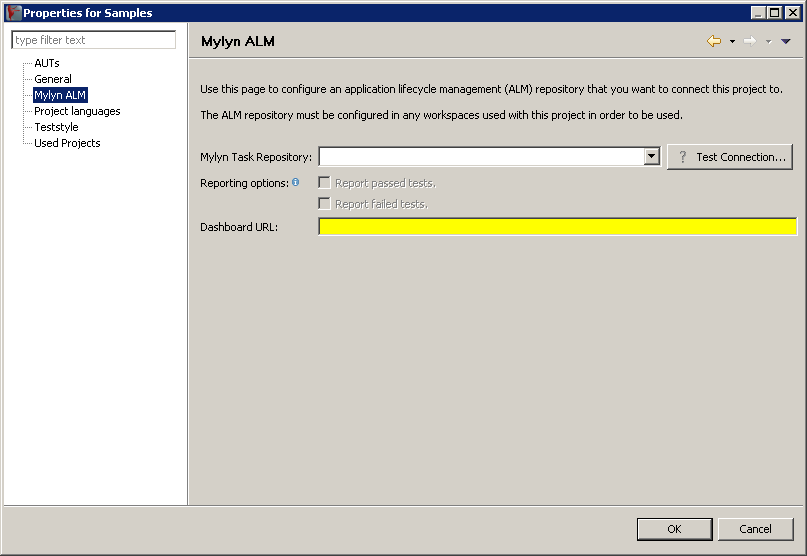
\includegraphics[width=12.5cm]{Tasks/ALM/PS/almproperties}
\caption{ALM Settings}
\label{TasksALMProjectProperties}
\end{center}
\end{figure}


\subsection{Adding task IDs to \gdjobs{}, \gdsuites{} and \gdcases{}}
\label{TasksALMAddTask}
You can add a task ID to \gdcases{}, \gdsuites{} and \gdjobs{} in your \gdproject{}. 

The task ID should be a valid ID in the repository that you have specified as the repository for this \gdproject{} \bxpref{TasksALMConfigureProject}. Adding the task ID to an item in your \gdproject{} means that this item is the relevant test for that task in your repository. When you activate the option, any test results for this item will be added as a comment to the task in the repository. The comment will include a link to the dashboard, in which the test result report can be viewed.

To add a task ID to a \gdcase{}, \gdsuite{} or \gdjob{}:
\begin{enumerate}
\item Open the item in the editor by double-clicking it.
\item In the \gdpropview{}, in the cell for \bxname{Task ID}, enter the task ID from the external repository. You can only enter task IDs at the place of specification -- you cannot overwrite them when you reuse the item.
\item Save the editor. 
\item When you have added a task ID to a node, you can open the task for this node from the browser by selecting:\\
\bxmenu{Open with}{Mylyn Task Editor}{}
\end{enumerate}

\bxtipp{You should ensure that you add task IDs to the right node-level to provide you with the relevant amount of information for the tasks in your repository. This will usually be at the level of Use Cases within a \gdsuite{}. }




\section{Starting the Integrated Test Environment (\ite{})}
The amount of keywords you have in a \app{} test and the amount of components your test deals with can grow very quickly. For this reason, it is important to think about structuring the \gdtestcasebrowser{} and the \gdomeditor{} to make finding \gdcases{} and component names easier. 


\subsection{Configuring task repositories in your workspace}
\label{TasksALMConfigureWorkspace}
Each repository you want to work with in your \ite{} must be configured in the workspace you are using. 

\begin{enumerate}
\item Select:\\ \bxmenu{Window}{Show View}{Other}\\ from the menu.
\item In the \bxname{Mylyn} section, select \bxname{Task Repositories} and click \bxcaption{OK}. The \bxname{Task Repositories} View will appear. The Bugzilla Repositories for \gd{} and \jb{} are pre-configured.
\item In the \bxname{Task Repositories} View, right click and select \bxname{Add Task Repository} from the context menu.
\item In the dialog that appears, you will see the pre-defined task repositories for the \ite{}. You can select one of these or choose to install a different connector. Depending on the connector you want to use, you may require additional software from Tasktop, or the connector may incur license fees.
\item Once you have selected your connector, click \bxcaption{Next}.
\item On the following page, you will need to configure the task repository. Please refer to the Mylyn documentation for information on repository configuration. 
\item Click \bxcaption{Finish} once the repository is configured.
\item To be able to see tasks in this repository, select: \\ \bxmenu{Window}{Show View}{Other}\\ from the menu. 
\item In the \bxname{Mylyn} section, select \bxname{Task List} and click \bxcaption{OK}. The \bxname{Task List} View will appear.
\end{enumerate}

You will now be able to see items in this repository, open them in the \ite{}, add queries for your workspace and work on tasks from this repository. 
You will also be able to select this repository in the \gdproject{} properties as the repository for your \gdproject{} \bxpref{TasksALMConfigureProject}. 


\subsection{Working on tasks in the \ite{}: contexts}
Once you have configured a task repository for your workspace \bxpref{TasksALMConfigureWorkspace}, you can work on tasks from that repository. 

\subsubsection{Opening and editing tasks in the \ite{}}
\begin{itemize}
\item To be able to see tasks in a repository, select: \\ \bxmenu{Window}{Show View}{Other}\\ from the menu. 
\item In the \bxname{Mylyn} section, select \bxname{Task List} and click \bxcaption{OK}. The \bxname{Task List} View will appear.
\item Double-click on a task to open this task in the editor area.
\item Once a task is open, you can work on it as you would in an external system -- add comments, change status etc.
\end{itemize}

\subsubsection{Working on tasks in the \ite{}}
\label{TasksActivateTask}
Mylyn supports context- or task-based working. When you work on a task, you only see items relevant to that task, so that coming back to the task later involves less context-switching. 
\begin{itemize}
\item Mylyn supports context-based working. You can work on existing tasks in a configured repository, or you can create tasks to work on.
\item To work on a task, you must \bxname{activate} it. To activate a task, select the task in the \bxname{Task List} and select:\\ \bxmenu{Activate}{}{}\\
from the context-sensitive menu. 
\item When you activate a task for the first time, the browsers and editors will seem very empty. This is because nothing is yet a part of the context for this task.
\item You can navigate through the browsers by pressing \bxkey{Alt+Click} to expand each level, or you can press the \bxname{Focus on task} button in the browsers to show the whole tree (not focusing on the task), or just the items in the current context (focusing on the task). 
\item Items are automatically added to your context when you select them in a browser, when you open them in an editor, or when you perform other actions that cause them to be made relevant (e.g. \gdcase{} creation, showing a \gdcase{} specification etc.). Items that are used particularly frequently are marked as \bxname{landmarks} and shown in bold. 
\item You can manually alter which items are in your context using the context-sensitive menu for a specific item. You can manually make items landmarks, or remove them from the context. 
\item The context that is created for you will be re-created when you reactivate the task at a later point. 
\end{itemize}



\subsection{Creating tasks in external repositories from test result reports}
\gdhelpid{testResultViewContextId}{Test Results View}
 You can create a new task with pre-filled information directly from an open test result report in the \gdtestresultview{}. This is useful if a test has failed and you want to create e.g. an issue in your bug-tracking system for the failure. 
\begin{enumerate}
\item In an open test result report, select the node that best describes the test failure (e.g. a \gdcase{} or \gdstep{} that has failed, or the whole \gdsuite{}, then right-click and select:\\
\bxmenu{Create a Mylyn Task}{}{}\\
from the context-sensitive menu.
\item  In the dialog that appears, select a repository in which to create the task. A \bxname{local} repository is available by default, but you can also add connections to Bugzilla and Trac repositories by clicking \bxcaption{Add Task Repository} in the New Task Dialog. Connectors to other repositories can also be added. See the Mylyn documentation for more details on adding repositories.
\item Click \bxcaption{Finish} once you have selected your repository. 
\item The editor for a new task will appear. It is pre-filled with information relevant to the node that you selected. Edit the task to make it descriptive enough for a bug report and save the editor. 
\item Once you have created a task, you can activate it to start saving your context for this task. See the later section \bxpref{TasksActivateTask} for details.
\end{enumerate}


\subsection{Configuring a task repository for your \gdproject{}}
\label{TasksALMConfigureProject}
Once you have configured one or more repositories for your workspace \bxpref{}, you can select one of these to be the test-relevant repository for your \gdproject{}. 

This will let you:
\begin{itemize}
\item Add a task ID from this repository to \gdcases{}, \gdsuites{}, and \gdjobs{} in the \gdproject{} to signify that this item is the test for this task \bxpref{TasksALMAddTask}.
\item Automatically report test results to the task defined when a test runs.
\item View the test results for the relevant item in the dashboard as a link from the task repository.
\end{itemize}

To configure a task repository for your \gdproject{}:

\begin{enumerate}
\item In the \gdproject{} Properties, select \bxname{Mylyn ALM} from the tree on the left \bxfigref{TasksALMProjectProperties}.
\item In the page that appears, you can select a repository from the combo-box.
\item You can then choose whether to only report failed tests, only report successful tests, or both.
\item Enter the URL of the \dash{} that is configured to use the correct \gddb{} for your test results. This is the \dash{} that will be opened when you click on a test result link from the task repository.
\end{enumerate}

\begin{figure}[h]
\begin{center}
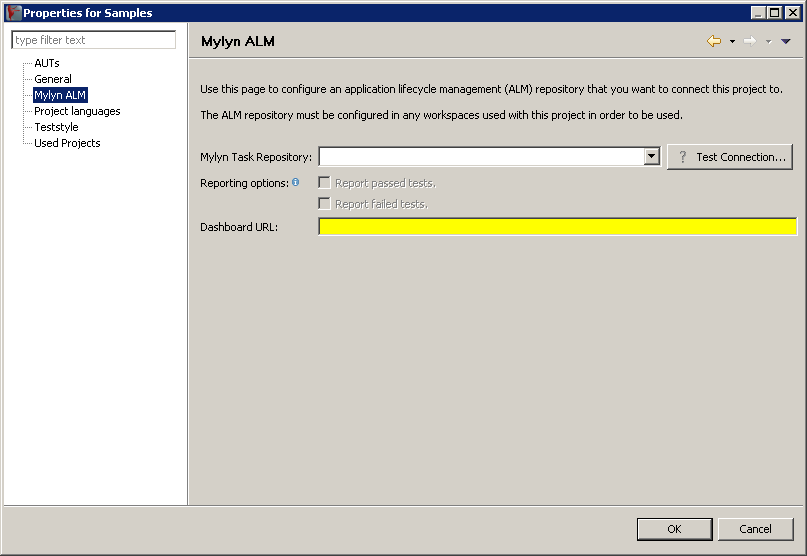
\includegraphics[width=12.5cm]{Tasks/ALM/PS/almproperties}
\caption{ALM Settings}
\label{TasksALMProjectProperties}
\end{center}
\end{figure}


\subsection{Adding task IDs to \gdjobs{}, \gdsuites{} and \gdcases{}}
\label{TasksALMAddTask}
You can add a task ID to \gdcases{}, \gdsuites{} and \gdjobs{} in your \gdproject{}. 

The task ID should be a valid ID in the repository that you have specified as the repository for this \gdproject{} \bxpref{TasksALMConfigureProject}. Adding the task ID to an item in your \gdproject{} means that this item is the relevant test for that task in your repository. When you activate the option, any test results for this item will be added as a comment to the task in the repository. The comment will include a link to the dashboard, in which the test result report can be viewed.

To add a task ID to a \gdcase{}, \gdsuite{} or \gdjob{}:
\begin{enumerate}
\item Open the item in the editor by double-clicking it.
\item In the \gdpropview{}, in the cell for \bxname{Task ID}, enter the task ID from the external repository. You can only enter task IDs at the place of specification -- you cannot overwrite them when you reuse the item.
\item Save the editor. 
\item When you have added a task ID to a node, you can open the task for this node from the browser by selecting:\\
\bxmenu{Open with}{Mylyn Task Editor}{}
\end{enumerate}

\bxtipp{You should ensure that you add task IDs to the right node-level to provide you with the relevant amount of information for the tasks in your repository. This will usually be at the level of Use Cases within a \gdsuite{}. }




\section{Logging into and switching databases}
\gdhelpid{dbLoginContextId}{Database Login}
The amount of keywords you have in a \app{} test and the amount of components your test deals with can grow very quickly. For this reason, it is important to think about structuring the \gdtestcasebrowser{} and the \gdomeditor{} to make finding \gdcases{} and component names easier. 


\subsection{Configuring task repositories in your workspace}
\label{TasksALMConfigureWorkspace}
Each repository you want to work with in your \ite{} must be configured in the workspace you are using. 

\begin{enumerate}
\item Select:\\ \bxmenu{Window}{Show View}{Other}\\ from the menu.
\item In the \bxname{Mylyn} section, select \bxname{Task Repositories} and click \bxcaption{OK}. The \bxname{Task Repositories} View will appear. The Bugzilla Repositories for \gd{} and \jb{} are pre-configured.
\item In the \bxname{Task Repositories} View, right click and select \bxname{Add Task Repository} from the context menu.
\item In the dialog that appears, you will see the pre-defined task repositories for the \ite{}. You can select one of these or choose to install a different connector. Depending on the connector you want to use, you may require additional software from Tasktop, or the connector may incur license fees.
\item Once you have selected your connector, click \bxcaption{Next}.
\item On the following page, you will need to configure the task repository. Please refer to the Mylyn documentation for information on repository configuration. 
\item Click \bxcaption{Finish} once the repository is configured.
\item To be able to see tasks in this repository, select: \\ \bxmenu{Window}{Show View}{Other}\\ from the menu. 
\item In the \bxname{Mylyn} section, select \bxname{Task List} and click \bxcaption{OK}. The \bxname{Task List} View will appear.
\end{enumerate}

You will now be able to see items in this repository, open them in the \ite{}, add queries for your workspace and work on tasks from this repository. 
You will also be able to select this repository in the \gdproject{} properties as the repository for your \gdproject{} \bxpref{TasksALMConfigureProject}. 


\subsection{Working on tasks in the \ite{}: contexts}
Once you have configured a task repository for your workspace \bxpref{TasksALMConfigureWorkspace}, you can work on tasks from that repository. 

\subsubsection{Opening and editing tasks in the \ite{}}
\begin{itemize}
\item To be able to see tasks in a repository, select: \\ \bxmenu{Window}{Show View}{Other}\\ from the menu. 
\item In the \bxname{Mylyn} section, select \bxname{Task List} and click \bxcaption{OK}. The \bxname{Task List} View will appear.
\item Double-click on a task to open this task in the editor area.
\item Once a task is open, you can work on it as you would in an external system -- add comments, change status etc.
\end{itemize}

\subsubsection{Working on tasks in the \ite{}}
\label{TasksActivateTask}
Mylyn supports context- or task-based working. When you work on a task, you only see items relevant to that task, so that coming back to the task later involves less context-switching. 
\begin{itemize}
\item Mylyn supports context-based working. You can work on existing tasks in a configured repository, or you can create tasks to work on.
\item To work on a task, you must \bxname{activate} it. To activate a task, select the task in the \bxname{Task List} and select:\\ \bxmenu{Activate}{}{}\\
from the context-sensitive menu. 
\item When you activate a task for the first time, the browsers and editors will seem very empty. This is because nothing is yet a part of the context for this task.
\item You can navigate through the browsers by pressing \bxkey{Alt+Click} to expand each level, or you can press the \bxname{Focus on task} button in the browsers to show the whole tree (not focusing on the task), or just the items in the current context (focusing on the task). 
\item Items are automatically added to your context when you select them in a browser, when you open them in an editor, or when you perform other actions that cause them to be made relevant (e.g. \gdcase{} creation, showing a \gdcase{} specification etc.). Items that are used particularly frequently are marked as \bxname{landmarks} and shown in bold. 
\item You can manually alter which items are in your context using the context-sensitive menu for a specific item. You can manually make items landmarks, or remove them from the context. 
\item The context that is created for you will be re-created when you reactivate the task at a later point. 
\end{itemize}



\subsection{Creating tasks in external repositories from test result reports}
\gdhelpid{testResultViewContextId}{Test Results View}
 You can create a new task with pre-filled information directly from an open test result report in the \gdtestresultview{}. This is useful if a test has failed and you want to create e.g. an issue in your bug-tracking system for the failure. 
\begin{enumerate}
\item In an open test result report, select the node that best describes the test failure (e.g. a \gdcase{} or \gdstep{} that has failed, or the whole \gdsuite{}, then right-click and select:\\
\bxmenu{Create a Mylyn Task}{}{}\\
from the context-sensitive menu.
\item  In the dialog that appears, select a repository in which to create the task. A \bxname{local} repository is available by default, but you can also add connections to Bugzilla and Trac repositories by clicking \bxcaption{Add Task Repository} in the New Task Dialog. Connectors to other repositories can also be added. See the Mylyn documentation for more details on adding repositories.
\item Click \bxcaption{Finish} once you have selected your repository. 
\item The editor for a new task will appear. It is pre-filled with information relevant to the node that you selected. Edit the task to make it descriptive enough for a bug report and save the editor. 
\item Once you have created a task, you can activate it to start saving your context for this task. See the later section \bxpref{TasksActivateTask} for details.
\end{enumerate}


\subsection{Configuring a task repository for your \gdproject{}}
\label{TasksALMConfigureProject}
Once you have configured one or more repositories for your workspace \bxpref{}, you can select one of these to be the test-relevant repository for your \gdproject{}. 

This will let you:
\begin{itemize}
\item Add a task ID from this repository to \gdcases{}, \gdsuites{}, and \gdjobs{} in the \gdproject{} to signify that this item is the test for this task \bxpref{TasksALMAddTask}.
\item Automatically report test results to the task defined when a test runs.
\item View the test results for the relevant item in the dashboard as a link from the task repository.
\end{itemize}

To configure a task repository for your \gdproject{}:

\begin{enumerate}
\item In the \gdproject{} Properties, select \bxname{Mylyn ALM} from the tree on the left \bxfigref{TasksALMProjectProperties}.
\item In the page that appears, you can select a repository from the combo-box.
\item You can then choose whether to only report failed tests, only report successful tests, or both.
\item Enter the URL of the \dash{} that is configured to use the correct \gddb{} for your test results. This is the \dash{} that will be opened when you click on a test result link from the task repository.
\end{enumerate}

\begin{figure}[h]
\begin{center}
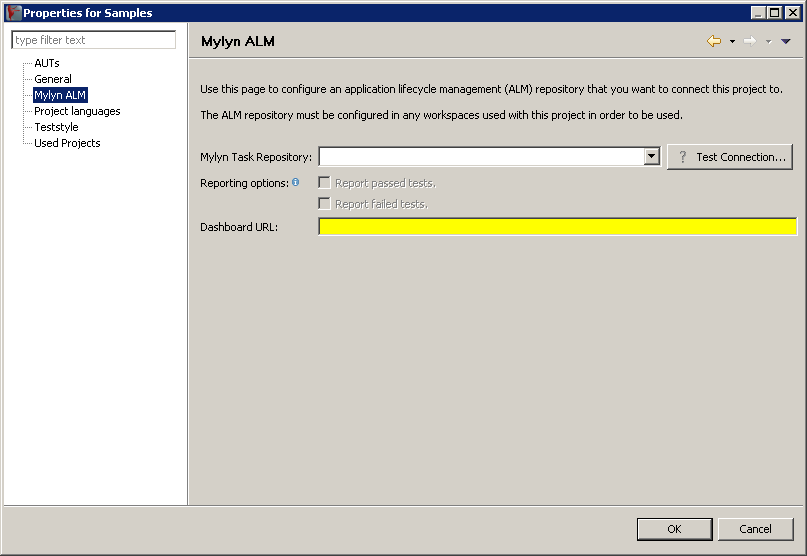
\includegraphics[width=12.5cm]{Tasks/ALM/PS/almproperties}
\caption{ALM Settings}
\label{TasksALMProjectProperties}
\end{center}
\end{figure}


\subsection{Adding task IDs to \gdjobs{}, \gdsuites{} and \gdcases{}}
\label{TasksALMAddTask}
You can add a task ID to \gdcases{}, \gdsuites{} and \gdjobs{} in your \gdproject{}. 

The task ID should be a valid ID in the repository that you have specified as the repository for this \gdproject{} \bxpref{TasksALMConfigureProject}. Adding the task ID to an item in your \gdproject{} means that this item is the relevant test for that task in your repository. When you activate the option, any test results for this item will be added as a comment to the task in the repository. The comment will include a link to the dashboard, in which the test result report can be viewed.

To add a task ID to a \gdcase{}, \gdsuite{} or \gdjob{}:
\begin{enumerate}
\item Open the item in the editor by double-clicking it.
\item In the \gdpropview{}, in the cell for \bxname{Task ID}, enter the task ID from the external repository. You can only enter task IDs at the place of specification -- you cannot overwrite them when you reuse the item.
\item Save the editor. 
\item When you have added a task ID to a node, you can open the task for this node from the browser by selecting:\\
\bxmenu{Open with}{Mylyn Task Editor}{}
\end{enumerate}

\bxtipp{You should ensure that you add task IDs to the right node-level to provide you with the relevant amount of information for the tasks in your repository. This will usually be at the level of Use Cases within a \gdsuite{}. }





\clearpage

\section{Working with \gdprojects{}}
\label{WorkingWithProjects}
The amount of keywords you have in a \app{} test and the amount of components your test deals with can grow very quickly. For this reason, it is important to think about structuring the \gdtestcasebrowser{} and the \gdomeditor{} to make finding \gdcases{} and component names easier. 


\subsection{Configuring task repositories in your workspace}
\label{TasksALMConfigureWorkspace}
Each repository you want to work with in your \ite{} must be configured in the workspace you are using. 

\begin{enumerate}
\item Select:\\ \bxmenu{Window}{Show View}{Other}\\ from the menu.
\item In the \bxname{Mylyn} section, select \bxname{Task Repositories} and click \bxcaption{OK}. The \bxname{Task Repositories} View will appear. The Bugzilla Repositories for \gd{} and \jb{} are pre-configured.
\item In the \bxname{Task Repositories} View, right click and select \bxname{Add Task Repository} from the context menu.
\item In the dialog that appears, you will see the pre-defined task repositories for the \ite{}. You can select one of these or choose to install a different connector. Depending on the connector you want to use, you may require additional software from Tasktop, or the connector may incur license fees.
\item Once you have selected your connector, click \bxcaption{Next}.
\item On the following page, you will need to configure the task repository. Please refer to the Mylyn documentation for information on repository configuration. 
\item Click \bxcaption{Finish} once the repository is configured.
\item To be able to see tasks in this repository, select: \\ \bxmenu{Window}{Show View}{Other}\\ from the menu. 
\item In the \bxname{Mylyn} section, select \bxname{Task List} and click \bxcaption{OK}. The \bxname{Task List} View will appear.
\end{enumerate}

You will now be able to see items in this repository, open them in the \ite{}, add queries for your workspace and work on tasks from this repository. 
You will also be able to select this repository in the \gdproject{} properties as the repository for your \gdproject{} \bxpref{TasksALMConfigureProject}. 


\subsection{Working on tasks in the \ite{}: contexts}
Once you have configured a task repository for your workspace \bxpref{TasksALMConfigureWorkspace}, you can work on tasks from that repository. 

\subsubsection{Opening and editing tasks in the \ite{}}
\begin{itemize}
\item To be able to see tasks in a repository, select: \\ \bxmenu{Window}{Show View}{Other}\\ from the menu. 
\item In the \bxname{Mylyn} section, select \bxname{Task List} and click \bxcaption{OK}. The \bxname{Task List} View will appear.
\item Double-click on a task to open this task in the editor area.
\item Once a task is open, you can work on it as you would in an external system -- add comments, change status etc.
\end{itemize}

\subsubsection{Working on tasks in the \ite{}}
\label{TasksActivateTask}
Mylyn supports context- or task-based working. When you work on a task, you only see items relevant to that task, so that coming back to the task later involves less context-switching. 
\begin{itemize}
\item Mylyn supports context-based working. You can work on existing tasks in a configured repository, or you can create tasks to work on.
\item To work on a task, you must \bxname{activate} it. To activate a task, select the task in the \bxname{Task List} and select:\\ \bxmenu{Activate}{}{}\\
from the context-sensitive menu. 
\item When you activate a task for the first time, the browsers and editors will seem very empty. This is because nothing is yet a part of the context for this task.
\item You can navigate through the browsers by pressing \bxkey{Alt+Click} to expand each level, or you can press the \bxname{Focus on task} button in the browsers to show the whole tree (not focusing on the task), or just the items in the current context (focusing on the task). 
\item Items are automatically added to your context when you select them in a browser, when you open them in an editor, or when you perform other actions that cause them to be made relevant (e.g. \gdcase{} creation, showing a \gdcase{} specification etc.). Items that are used particularly frequently are marked as \bxname{landmarks} and shown in bold. 
\item You can manually alter which items are in your context using the context-sensitive menu for a specific item. You can manually make items landmarks, or remove them from the context. 
\item The context that is created for you will be re-created when you reactivate the task at a later point. 
\end{itemize}



\subsection{Creating tasks in external repositories from test result reports}
\gdhelpid{testResultViewContextId}{Test Results View}
 You can create a new task with pre-filled information directly from an open test result report in the \gdtestresultview{}. This is useful if a test has failed and you want to create e.g. an issue in your bug-tracking system for the failure. 
\begin{enumerate}
\item In an open test result report, select the node that best describes the test failure (e.g. a \gdcase{} or \gdstep{} that has failed, or the whole \gdsuite{}, then right-click and select:\\
\bxmenu{Create a Mylyn Task}{}{}\\
from the context-sensitive menu.
\item  In the dialog that appears, select a repository in which to create the task. A \bxname{local} repository is available by default, but you can also add connections to Bugzilla and Trac repositories by clicking \bxcaption{Add Task Repository} in the New Task Dialog. Connectors to other repositories can also be added. See the Mylyn documentation for more details on adding repositories.
\item Click \bxcaption{Finish} once you have selected your repository. 
\item The editor for a new task will appear. It is pre-filled with information relevant to the node that you selected. Edit the task to make it descriptive enough for a bug report and save the editor. 
\item Once you have created a task, you can activate it to start saving your context for this task. See the later section \bxpref{TasksActivateTask} for details.
\end{enumerate}


\subsection{Configuring a task repository for your \gdproject{}}
\label{TasksALMConfigureProject}
Once you have configured one or more repositories for your workspace \bxpref{}, you can select one of these to be the test-relevant repository for your \gdproject{}. 

This will let you:
\begin{itemize}
\item Add a task ID from this repository to \gdcases{}, \gdsuites{}, and \gdjobs{} in the \gdproject{} to signify that this item is the test for this task \bxpref{TasksALMAddTask}.
\item Automatically report test results to the task defined when a test runs.
\item View the test results for the relevant item in the dashboard as a link from the task repository.
\end{itemize}

To configure a task repository for your \gdproject{}:

\begin{enumerate}
\item In the \gdproject{} Properties, select \bxname{Mylyn ALM} from the tree on the left \bxfigref{TasksALMProjectProperties}.
\item In the page that appears, you can select a repository from the combo-box.
\item You can then choose whether to only report failed tests, only report successful tests, or both.
\item Enter the URL of the \dash{} that is configured to use the correct \gddb{} for your test results. This is the \dash{} that will be opened when you click on a test result link from the task repository.
\end{enumerate}

\begin{figure}[h]
\begin{center}
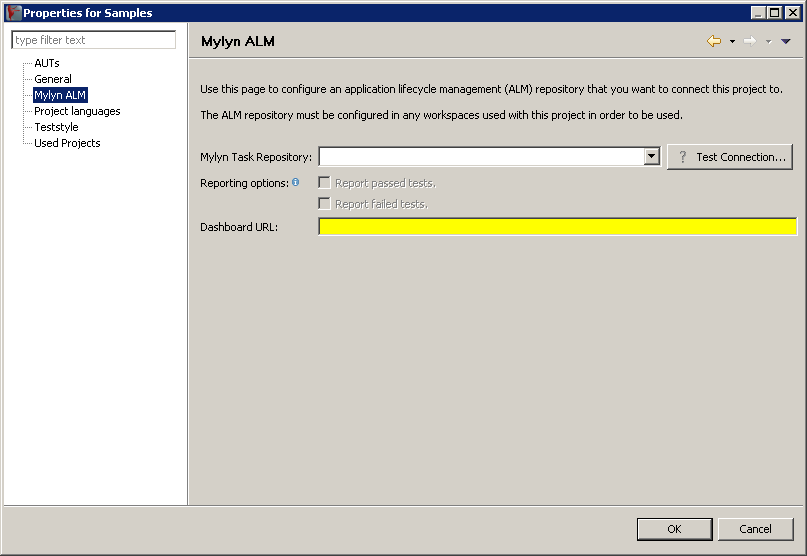
\includegraphics[width=12.5cm]{Tasks/ALM/PS/almproperties}
\caption{ALM Settings}
\label{TasksALMProjectProperties}
\end{center}
\end{figure}


\subsection{Adding task IDs to \gdjobs{}, \gdsuites{} and \gdcases{}}
\label{TasksALMAddTask}
You can add a task ID to \gdcases{}, \gdsuites{} and \gdjobs{} in your \gdproject{}. 

The task ID should be a valid ID in the repository that you have specified as the repository for this \gdproject{} \bxpref{TasksALMConfigureProject}. Adding the task ID to an item in your \gdproject{} means that this item is the relevant test for that task in your repository. When you activate the option, any test results for this item will be added as a comment to the task in the repository. The comment will include a link to the dashboard, in which the test result report can be viewed.

To add a task ID to a \gdcase{}, \gdsuite{} or \gdjob{}:
\begin{enumerate}
\item Open the item in the editor by double-clicking it.
\item In the \gdpropview{}, in the cell for \bxname{Task ID}, enter the task ID from the external repository. You can only enter task IDs at the place of specification -- you cannot overwrite them when you reuse the item.
\item Save the editor. 
\item When you have added a task ID to a node, you can open the task for this node from the browser by selecting:\\
\bxmenu{Open with}{Mylyn Task Editor}{}
\end{enumerate}

\bxtipp{You should ensure that you add task IDs to the right node-level to provide you with the relevant amount of information for the tasks in your repository. This will usually be at the level of Use Cases within a \gdsuite{}. }




\clearpage
\section{Starting and configuring \gdauts{}}
\label{StartAUT}
The amount of keywords you have in a \app{} test and the amount of components your test deals with can grow very quickly. For this reason, it is important to think about structuring the \gdtestcasebrowser{} and the \gdomeditor{} to make finding \gdcases{} and component names easier. 


\subsection{Configuring task repositories in your workspace}
\label{TasksALMConfigureWorkspace}
Each repository you want to work with in your \ite{} must be configured in the workspace you are using. 

\begin{enumerate}
\item Select:\\ \bxmenu{Window}{Show View}{Other}\\ from the menu.
\item In the \bxname{Mylyn} section, select \bxname{Task Repositories} and click \bxcaption{OK}. The \bxname{Task Repositories} View will appear. The Bugzilla Repositories for \gd{} and \jb{} are pre-configured.
\item In the \bxname{Task Repositories} View, right click and select \bxname{Add Task Repository} from the context menu.
\item In the dialog that appears, you will see the pre-defined task repositories for the \ite{}. You can select one of these or choose to install a different connector. Depending on the connector you want to use, you may require additional software from Tasktop, or the connector may incur license fees.
\item Once you have selected your connector, click \bxcaption{Next}.
\item On the following page, you will need to configure the task repository. Please refer to the Mylyn documentation for information on repository configuration. 
\item Click \bxcaption{Finish} once the repository is configured.
\item To be able to see tasks in this repository, select: \\ \bxmenu{Window}{Show View}{Other}\\ from the menu. 
\item In the \bxname{Mylyn} section, select \bxname{Task List} and click \bxcaption{OK}. The \bxname{Task List} View will appear.
\end{enumerate}

You will now be able to see items in this repository, open them in the \ite{}, add queries for your workspace and work on tasks from this repository. 
You will also be able to select this repository in the \gdproject{} properties as the repository for your \gdproject{} \bxpref{TasksALMConfigureProject}. 


\subsection{Working on tasks in the \ite{}: contexts}
Once you have configured a task repository for your workspace \bxpref{TasksALMConfigureWorkspace}, you can work on tasks from that repository. 

\subsubsection{Opening and editing tasks in the \ite{}}
\begin{itemize}
\item To be able to see tasks in a repository, select: \\ \bxmenu{Window}{Show View}{Other}\\ from the menu. 
\item In the \bxname{Mylyn} section, select \bxname{Task List} and click \bxcaption{OK}. The \bxname{Task List} View will appear.
\item Double-click on a task to open this task in the editor area.
\item Once a task is open, you can work on it as you would in an external system -- add comments, change status etc.
\end{itemize}

\subsubsection{Working on tasks in the \ite{}}
\label{TasksActivateTask}
Mylyn supports context- or task-based working. When you work on a task, you only see items relevant to that task, so that coming back to the task later involves less context-switching. 
\begin{itemize}
\item Mylyn supports context-based working. You can work on existing tasks in a configured repository, or you can create tasks to work on.
\item To work on a task, you must \bxname{activate} it. To activate a task, select the task in the \bxname{Task List} and select:\\ \bxmenu{Activate}{}{}\\
from the context-sensitive menu. 
\item When you activate a task for the first time, the browsers and editors will seem very empty. This is because nothing is yet a part of the context for this task.
\item You can navigate through the browsers by pressing \bxkey{Alt+Click} to expand each level, or you can press the \bxname{Focus on task} button in the browsers to show the whole tree (not focusing on the task), or just the items in the current context (focusing on the task). 
\item Items are automatically added to your context when you select them in a browser, when you open them in an editor, or when you perform other actions that cause them to be made relevant (e.g. \gdcase{} creation, showing a \gdcase{} specification etc.). Items that are used particularly frequently are marked as \bxname{landmarks} and shown in bold. 
\item You can manually alter which items are in your context using the context-sensitive menu for a specific item. You can manually make items landmarks, or remove them from the context. 
\item The context that is created for you will be re-created when you reactivate the task at a later point. 
\end{itemize}



\subsection{Creating tasks in external repositories from test result reports}
\gdhelpid{testResultViewContextId}{Test Results View}
 You can create a new task with pre-filled information directly from an open test result report in the \gdtestresultview{}. This is useful if a test has failed and you want to create e.g. an issue in your bug-tracking system for the failure. 
\begin{enumerate}
\item In an open test result report, select the node that best describes the test failure (e.g. a \gdcase{} or \gdstep{} that has failed, or the whole \gdsuite{}, then right-click and select:\\
\bxmenu{Create a Mylyn Task}{}{}\\
from the context-sensitive menu.
\item  In the dialog that appears, select a repository in which to create the task. A \bxname{local} repository is available by default, but you can also add connections to Bugzilla and Trac repositories by clicking \bxcaption{Add Task Repository} in the New Task Dialog. Connectors to other repositories can also be added. See the Mylyn documentation for more details on adding repositories.
\item Click \bxcaption{Finish} once you have selected your repository. 
\item The editor for a new task will appear. It is pre-filled with information relevant to the node that you selected. Edit the task to make it descriptive enough for a bug report and save the editor. 
\item Once you have created a task, you can activate it to start saving your context for this task. See the later section \bxpref{TasksActivateTask} for details.
\end{enumerate}


\subsection{Configuring a task repository for your \gdproject{}}
\label{TasksALMConfigureProject}
Once you have configured one or more repositories for your workspace \bxpref{}, you can select one of these to be the test-relevant repository for your \gdproject{}. 

This will let you:
\begin{itemize}
\item Add a task ID from this repository to \gdcases{}, \gdsuites{}, and \gdjobs{} in the \gdproject{} to signify that this item is the test for this task \bxpref{TasksALMAddTask}.
\item Automatically report test results to the task defined when a test runs.
\item View the test results for the relevant item in the dashboard as a link from the task repository.
\end{itemize}

To configure a task repository for your \gdproject{}:

\begin{enumerate}
\item In the \gdproject{} Properties, select \bxname{Mylyn ALM} from the tree on the left \bxfigref{TasksALMProjectProperties}.
\item In the page that appears, you can select a repository from the combo-box.
\item You can then choose whether to only report failed tests, only report successful tests, or both.
\item Enter the URL of the \dash{} that is configured to use the correct \gddb{} for your test results. This is the \dash{} that will be opened when you click on a test result link from the task repository.
\end{enumerate}

\begin{figure}[h]
\begin{center}
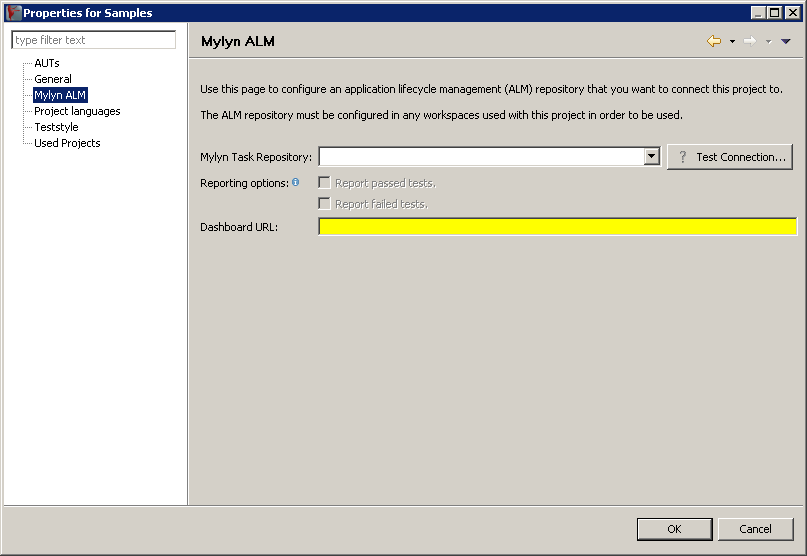
\includegraphics[width=12.5cm]{Tasks/ALM/PS/almproperties}
\caption{ALM Settings}
\label{TasksALMProjectProperties}
\end{center}
\end{figure}


\subsection{Adding task IDs to \gdjobs{}, \gdsuites{} and \gdcases{}}
\label{TasksALMAddTask}
You can add a task ID to \gdcases{}, \gdsuites{} and \gdjobs{} in your \gdproject{}. 

The task ID should be a valid ID in the repository that you have specified as the repository for this \gdproject{} \bxpref{TasksALMConfigureProject}. Adding the task ID to an item in your \gdproject{} means that this item is the relevant test for that task in your repository. When you activate the option, any test results for this item will be added as a comment to the task in the repository. The comment will include a link to the dashboard, in which the test result report can be viewed.

To add a task ID to a \gdcase{}, \gdsuite{} or \gdjob{}:
\begin{enumerate}
\item Open the item in the editor by double-clicking it.
\item In the \gdpropview{}, in the cell for \bxname{Task ID}, enter the task ID from the external repository. You can only enter task IDs at the place of specification -- you cannot overwrite them when you reuse the item.
\item Save the editor. 
\item When you have added a task ID to a node, you can open the task for this node from the browser by selecting:\\
\bxmenu{Open with}{Mylyn Task Editor}{}
\end{enumerate}

\bxtipp{You should ensure that you add task IDs to the right node-level to provide you with the relevant amount of information for the tasks in your repository. This will usually be at the level of Use Cases within a \gdsuite{}. }




\clearpage
\section{Working with browsers}
\label{WorkingWithBrowsers}
The amount of keywords you have in a \app{} test and the amount of components your test deals with can grow very quickly. For this reason, it is important to think about structuring the \gdtestcasebrowser{} and the \gdomeditor{} to make finding \gdcases{} and component names easier. 


\subsection{Configuring task repositories in your workspace}
\label{TasksALMConfigureWorkspace}
Each repository you want to work with in your \ite{} must be configured in the workspace you are using. 

\begin{enumerate}
\item Select:\\ \bxmenu{Window}{Show View}{Other}\\ from the menu.
\item In the \bxname{Mylyn} section, select \bxname{Task Repositories} and click \bxcaption{OK}. The \bxname{Task Repositories} View will appear. The Bugzilla Repositories for \gd{} and \jb{} are pre-configured.
\item In the \bxname{Task Repositories} View, right click and select \bxname{Add Task Repository} from the context menu.
\item In the dialog that appears, you will see the pre-defined task repositories for the \ite{}. You can select one of these or choose to install a different connector. Depending on the connector you want to use, you may require additional software from Tasktop, or the connector may incur license fees.
\item Once you have selected your connector, click \bxcaption{Next}.
\item On the following page, you will need to configure the task repository. Please refer to the Mylyn documentation for information on repository configuration. 
\item Click \bxcaption{Finish} once the repository is configured.
\item To be able to see tasks in this repository, select: \\ \bxmenu{Window}{Show View}{Other}\\ from the menu. 
\item In the \bxname{Mylyn} section, select \bxname{Task List} and click \bxcaption{OK}. The \bxname{Task List} View will appear.
\end{enumerate}

You will now be able to see items in this repository, open them in the \ite{}, add queries for your workspace and work on tasks from this repository. 
You will also be able to select this repository in the \gdproject{} properties as the repository for your \gdproject{} \bxpref{TasksALMConfigureProject}. 


\subsection{Working on tasks in the \ite{}: contexts}
Once you have configured a task repository for your workspace \bxpref{TasksALMConfigureWorkspace}, you can work on tasks from that repository. 

\subsubsection{Opening and editing tasks in the \ite{}}
\begin{itemize}
\item To be able to see tasks in a repository, select: \\ \bxmenu{Window}{Show View}{Other}\\ from the menu. 
\item In the \bxname{Mylyn} section, select \bxname{Task List} and click \bxcaption{OK}. The \bxname{Task List} View will appear.
\item Double-click on a task to open this task in the editor area.
\item Once a task is open, you can work on it as you would in an external system -- add comments, change status etc.
\end{itemize}

\subsubsection{Working on tasks in the \ite{}}
\label{TasksActivateTask}
Mylyn supports context- or task-based working. When you work on a task, you only see items relevant to that task, so that coming back to the task later involves less context-switching. 
\begin{itemize}
\item Mylyn supports context-based working. You can work on existing tasks in a configured repository, or you can create tasks to work on.
\item To work on a task, you must \bxname{activate} it. To activate a task, select the task in the \bxname{Task List} and select:\\ \bxmenu{Activate}{}{}\\
from the context-sensitive menu. 
\item When you activate a task for the first time, the browsers and editors will seem very empty. This is because nothing is yet a part of the context for this task.
\item You can navigate through the browsers by pressing \bxkey{Alt+Click} to expand each level, or you can press the \bxname{Focus on task} button in the browsers to show the whole tree (not focusing on the task), or just the items in the current context (focusing on the task). 
\item Items are automatically added to your context when you select them in a browser, when you open them in an editor, or when you perform other actions that cause them to be made relevant (e.g. \gdcase{} creation, showing a \gdcase{} specification etc.). Items that are used particularly frequently are marked as \bxname{landmarks} and shown in bold. 
\item You can manually alter which items are in your context using the context-sensitive menu for a specific item. You can manually make items landmarks, or remove them from the context. 
\item The context that is created for you will be re-created when you reactivate the task at a later point. 
\end{itemize}



\subsection{Creating tasks in external repositories from test result reports}
\gdhelpid{testResultViewContextId}{Test Results View}
 You can create a new task with pre-filled information directly from an open test result report in the \gdtestresultview{}. This is useful if a test has failed and you want to create e.g. an issue in your bug-tracking system for the failure. 
\begin{enumerate}
\item In an open test result report, select the node that best describes the test failure (e.g. a \gdcase{} or \gdstep{} that has failed, or the whole \gdsuite{}, then right-click and select:\\
\bxmenu{Create a Mylyn Task}{}{}\\
from the context-sensitive menu.
\item  In the dialog that appears, select a repository in which to create the task. A \bxname{local} repository is available by default, but you can also add connections to Bugzilla and Trac repositories by clicking \bxcaption{Add Task Repository} in the New Task Dialog. Connectors to other repositories can also be added. See the Mylyn documentation for more details on adding repositories.
\item Click \bxcaption{Finish} once you have selected your repository. 
\item The editor for a new task will appear. It is pre-filled with information relevant to the node that you selected. Edit the task to make it descriptive enough for a bug report and save the editor. 
\item Once you have created a task, you can activate it to start saving your context for this task. See the later section \bxpref{TasksActivateTask} for details.
\end{enumerate}


\subsection{Configuring a task repository for your \gdproject{}}
\label{TasksALMConfigureProject}
Once you have configured one or more repositories for your workspace \bxpref{}, you can select one of these to be the test-relevant repository for your \gdproject{}. 

This will let you:
\begin{itemize}
\item Add a task ID from this repository to \gdcases{}, \gdsuites{}, and \gdjobs{} in the \gdproject{} to signify that this item is the test for this task \bxpref{TasksALMAddTask}.
\item Automatically report test results to the task defined when a test runs.
\item View the test results for the relevant item in the dashboard as a link from the task repository.
\end{itemize}

To configure a task repository for your \gdproject{}:

\begin{enumerate}
\item In the \gdproject{} Properties, select \bxname{Mylyn ALM} from the tree on the left \bxfigref{TasksALMProjectProperties}.
\item In the page that appears, you can select a repository from the combo-box.
\item You can then choose whether to only report failed tests, only report successful tests, or both.
\item Enter the URL of the \dash{} that is configured to use the correct \gddb{} for your test results. This is the \dash{} that will be opened when you click on a test result link from the task repository.
\end{enumerate}

\begin{figure}[h]
\begin{center}
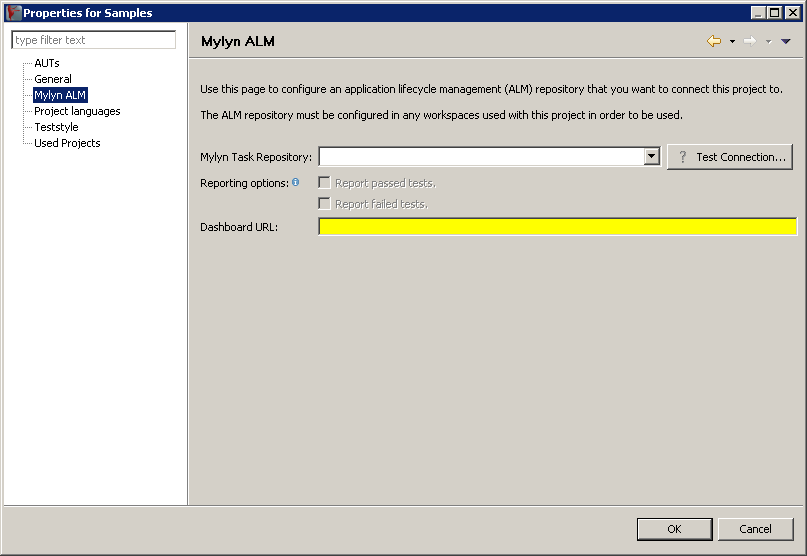
\includegraphics[width=12.5cm]{Tasks/ALM/PS/almproperties}
\caption{ALM Settings}
\label{TasksALMProjectProperties}
\end{center}
\end{figure}


\subsection{Adding task IDs to \gdjobs{}, \gdsuites{} and \gdcases{}}
\label{TasksALMAddTask}
You can add a task ID to \gdcases{}, \gdsuites{} and \gdjobs{} in your \gdproject{}. 

The task ID should be a valid ID in the repository that you have specified as the repository for this \gdproject{} \bxpref{TasksALMConfigureProject}. Adding the task ID to an item in your \gdproject{} means that this item is the relevant test for that task in your repository. When you activate the option, any test results for this item will be added as a comment to the task in the repository. The comment will include a link to the dashboard, in which the test result report can be viewed.

To add a task ID to a \gdcase{}, \gdsuite{} or \gdjob{}:
\begin{enumerate}
\item Open the item in the editor by double-clicking it.
\item In the \gdpropview{}, in the cell for \bxname{Task ID}, enter the task ID from the external repository. You can only enter task IDs at the place of specification -- you cannot overwrite them when you reuse the item.
\item Save the editor. 
\item When you have added a task ID to a node, you can open the task for this node from the browser by selecting:\\
\bxmenu{Open with}{Mylyn Task Editor}{}
\end{enumerate}

\bxtipp{You should ensure that you add task IDs to the right node-level to provide you with the relevant amount of information for the tasks in your repository. This will usually be at the level of Use Cases within a \gdsuite{}. }




\section{Working with editors}
\label{WorkingWithEditors}
The amount of keywords you have in a \app{} test and the amount of components your test deals with can grow very quickly. For this reason, it is important to think about structuring the \gdtestcasebrowser{} and the \gdomeditor{} to make finding \gdcases{} and component names easier. 


\subsection{Configuring task repositories in your workspace}
\label{TasksALMConfigureWorkspace}
Each repository you want to work with in your \ite{} must be configured in the workspace you are using. 

\begin{enumerate}
\item Select:\\ \bxmenu{Window}{Show View}{Other}\\ from the menu.
\item In the \bxname{Mylyn} section, select \bxname{Task Repositories} and click \bxcaption{OK}. The \bxname{Task Repositories} View will appear. The Bugzilla Repositories for \gd{} and \jb{} are pre-configured.
\item In the \bxname{Task Repositories} View, right click and select \bxname{Add Task Repository} from the context menu.
\item In the dialog that appears, you will see the pre-defined task repositories for the \ite{}. You can select one of these or choose to install a different connector. Depending on the connector you want to use, you may require additional software from Tasktop, or the connector may incur license fees.
\item Once you have selected your connector, click \bxcaption{Next}.
\item On the following page, you will need to configure the task repository. Please refer to the Mylyn documentation for information on repository configuration. 
\item Click \bxcaption{Finish} once the repository is configured.
\item To be able to see tasks in this repository, select: \\ \bxmenu{Window}{Show View}{Other}\\ from the menu. 
\item In the \bxname{Mylyn} section, select \bxname{Task List} and click \bxcaption{OK}. The \bxname{Task List} View will appear.
\end{enumerate}

You will now be able to see items in this repository, open them in the \ite{}, add queries for your workspace and work on tasks from this repository. 
You will also be able to select this repository in the \gdproject{} properties as the repository for your \gdproject{} \bxpref{TasksALMConfigureProject}. 


\subsection{Working on tasks in the \ite{}: contexts}
Once you have configured a task repository for your workspace \bxpref{TasksALMConfigureWorkspace}, you can work on tasks from that repository. 

\subsubsection{Opening and editing tasks in the \ite{}}
\begin{itemize}
\item To be able to see tasks in a repository, select: \\ \bxmenu{Window}{Show View}{Other}\\ from the menu. 
\item In the \bxname{Mylyn} section, select \bxname{Task List} and click \bxcaption{OK}. The \bxname{Task List} View will appear.
\item Double-click on a task to open this task in the editor area.
\item Once a task is open, you can work on it as you would in an external system -- add comments, change status etc.
\end{itemize}

\subsubsection{Working on tasks in the \ite{}}
\label{TasksActivateTask}
Mylyn supports context- or task-based working. When you work on a task, you only see items relevant to that task, so that coming back to the task later involves less context-switching. 
\begin{itemize}
\item Mylyn supports context-based working. You can work on existing tasks in a configured repository, or you can create tasks to work on.
\item To work on a task, you must \bxname{activate} it. To activate a task, select the task in the \bxname{Task List} and select:\\ \bxmenu{Activate}{}{}\\
from the context-sensitive menu. 
\item When you activate a task for the first time, the browsers and editors will seem very empty. This is because nothing is yet a part of the context for this task.
\item You can navigate through the browsers by pressing \bxkey{Alt+Click} to expand each level, or you can press the \bxname{Focus on task} button in the browsers to show the whole tree (not focusing on the task), or just the items in the current context (focusing on the task). 
\item Items are automatically added to your context when you select them in a browser, when you open them in an editor, or when you perform other actions that cause them to be made relevant (e.g. \gdcase{} creation, showing a \gdcase{} specification etc.). Items that are used particularly frequently are marked as \bxname{landmarks} and shown in bold. 
\item You can manually alter which items are in your context using the context-sensitive menu for a specific item. You can manually make items landmarks, or remove them from the context. 
\item The context that is created for you will be re-created when you reactivate the task at a later point. 
\end{itemize}



\subsection{Creating tasks in external repositories from test result reports}
\gdhelpid{testResultViewContextId}{Test Results View}
 You can create a new task with pre-filled information directly from an open test result report in the \gdtestresultview{}. This is useful if a test has failed and you want to create e.g. an issue in your bug-tracking system for the failure. 
\begin{enumerate}
\item In an open test result report, select the node that best describes the test failure (e.g. a \gdcase{} or \gdstep{} that has failed, or the whole \gdsuite{}, then right-click and select:\\
\bxmenu{Create a Mylyn Task}{}{}\\
from the context-sensitive menu.
\item  In the dialog that appears, select a repository in which to create the task. A \bxname{local} repository is available by default, but you can also add connections to Bugzilla and Trac repositories by clicking \bxcaption{Add Task Repository} in the New Task Dialog. Connectors to other repositories can also be added. See the Mylyn documentation for more details on adding repositories.
\item Click \bxcaption{Finish} once you have selected your repository. 
\item The editor for a new task will appear. It is pre-filled with information relevant to the node that you selected. Edit the task to make it descriptive enough for a bug report and save the editor. 
\item Once you have created a task, you can activate it to start saving your context for this task. See the later section \bxpref{TasksActivateTask} for details.
\end{enumerate}


\subsection{Configuring a task repository for your \gdproject{}}
\label{TasksALMConfigureProject}
Once you have configured one or more repositories for your workspace \bxpref{}, you can select one of these to be the test-relevant repository for your \gdproject{}. 

This will let you:
\begin{itemize}
\item Add a task ID from this repository to \gdcases{}, \gdsuites{}, and \gdjobs{} in the \gdproject{} to signify that this item is the test for this task \bxpref{TasksALMAddTask}.
\item Automatically report test results to the task defined when a test runs.
\item View the test results for the relevant item in the dashboard as a link from the task repository.
\end{itemize}

To configure a task repository for your \gdproject{}:

\begin{enumerate}
\item In the \gdproject{} Properties, select \bxname{Mylyn ALM} from the tree on the left \bxfigref{TasksALMProjectProperties}.
\item In the page that appears, you can select a repository from the combo-box.
\item You can then choose whether to only report failed tests, only report successful tests, or both.
\item Enter the URL of the \dash{} that is configured to use the correct \gddb{} for your test results. This is the \dash{} that will be opened when you click on a test result link from the task repository.
\end{enumerate}

\begin{figure}[h]
\begin{center}
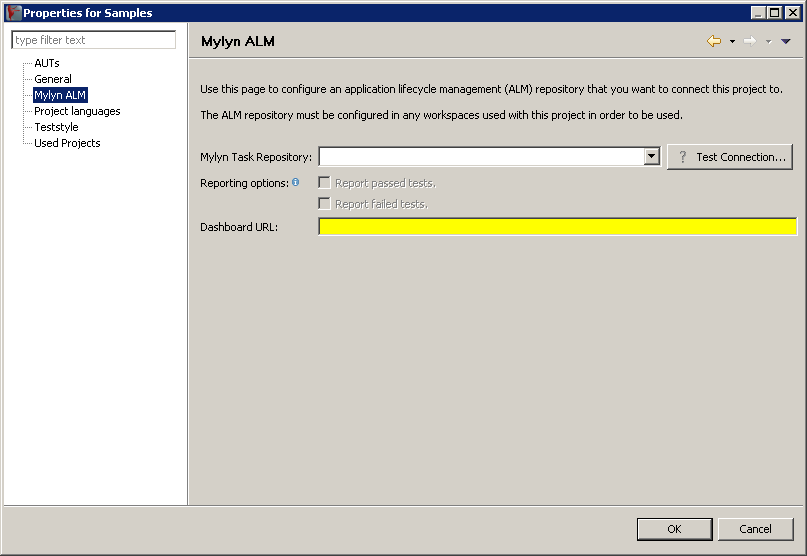
\includegraphics[width=12.5cm]{Tasks/ALM/PS/almproperties}
\caption{ALM Settings}
\label{TasksALMProjectProperties}
\end{center}
\end{figure}


\subsection{Adding task IDs to \gdjobs{}, \gdsuites{} and \gdcases{}}
\label{TasksALMAddTask}
You can add a task ID to \gdcases{}, \gdsuites{} and \gdjobs{} in your \gdproject{}. 

The task ID should be a valid ID in the repository that you have specified as the repository for this \gdproject{} \bxpref{TasksALMConfigureProject}. Adding the task ID to an item in your \gdproject{} means that this item is the relevant test for that task in your repository. When you activate the option, any test results for this item will be added as a comment to the task in the repository. The comment will include a link to the dashboard, in which the test result report can be viewed.

To add a task ID to a \gdcase{}, \gdsuite{} or \gdjob{}:
\begin{enumerate}
\item Open the item in the editor by double-clicking it.
\item In the \gdpropview{}, in the cell for \bxname{Task ID}, enter the task ID from the external repository. You can only enter task IDs at the place of specification -- you cannot overwrite them when you reuse the item.
\item Save the editor. 
\item When you have added a task ID to a node, you can open the task for this node from the browser by selecting:\\
\bxmenu{Open with}{Mylyn Task Editor}{}
\end{enumerate}

\bxtipp{You should ensure that you add task IDs to the right node-level to provide you with the relevant amount of information for the tasks in your repository. This will usually be at the level of Use Cases within a \gdsuite{}. }




\clearpage
\section{Working with \gdcases{}}
\gdhelpid{testSpecificationViewContextId}{Test Case Browser}
\gdhelpid{problemViewContextId}{Problem View}
\label{WorkingWithTestCases}
The amount of keywords you have in a \app{} test and the amount of components your test deals with can grow very quickly. For this reason, it is important to think about structuring the \gdtestcasebrowser{} and the \gdomeditor{} to make finding \gdcases{} and component names easier. 


\subsection{Configuring task repositories in your workspace}
\label{TasksALMConfigureWorkspace}
Each repository you want to work with in your \ite{} must be configured in the workspace you are using. 

\begin{enumerate}
\item Select:\\ \bxmenu{Window}{Show View}{Other}\\ from the menu.
\item In the \bxname{Mylyn} section, select \bxname{Task Repositories} and click \bxcaption{OK}. The \bxname{Task Repositories} View will appear. The Bugzilla Repositories for \gd{} and \jb{} are pre-configured.
\item In the \bxname{Task Repositories} View, right click and select \bxname{Add Task Repository} from the context menu.
\item In the dialog that appears, you will see the pre-defined task repositories for the \ite{}. You can select one of these or choose to install a different connector. Depending on the connector you want to use, you may require additional software from Tasktop, or the connector may incur license fees.
\item Once you have selected your connector, click \bxcaption{Next}.
\item On the following page, you will need to configure the task repository. Please refer to the Mylyn documentation for information on repository configuration. 
\item Click \bxcaption{Finish} once the repository is configured.
\item To be able to see tasks in this repository, select: \\ \bxmenu{Window}{Show View}{Other}\\ from the menu. 
\item In the \bxname{Mylyn} section, select \bxname{Task List} and click \bxcaption{OK}. The \bxname{Task List} View will appear.
\end{enumerate}

You will now be able to see items in this repository, open them in the \ite{}, add queries for your workspace and work on tasks from this repository. 
You will also be able to select this repository in the \gdproject{} properties as the repository for your \gdproject{} \bxpref{TasksALMConfigureProject}. 


\subsection{Working on tasks in the \ite{}: contexts}
Once you have configured a task repository for your workspace \bxpref{TasksALMConfigureWorkspace}, you can work on tasks from that repository. 

\subsubsection{Opening and editing tasks in the \ite{}}
\begin{itemize}
\item To be able to see tasks in a repository, select: \\ \bxmenu{Window}{Show View}{Other}\\ from the menu. 
\item In the \bxname{Mylyn} section, select \bxname{Task List} and click \bxcaption{OK}. The \bxname{Task List} View will appear.
\item Double-click on a task to open this task in the editor area.
\item Once a task is open, you can work on it as you would in an external system -- add comments, change status etc.
\end{itemize}

\subsubsection{Working on tasks in the \ite{}}
\label{TasksActivateTask}
Mylyn supports context- or task-based working. When you work on a task, you only see items relevant to that task, so that coming back to the task later involves less context-switching. 
\begin{itemize}
\item Mylyn supports context-based working. You can work on existing tasks in a configured repository, or you can create tasks to work on.
\item To work on a task, you must \bxname{activate} it. To activate a task, select the task in the \bxname{Task List} and select:\\ \bxmenu{Activate}{}{}\\
from the context-sensitive menu. 
\item When you activate a task for the first time, the browsers and editors will seem very empty. This is because nothing is yet a part of the context for this task.
\item You can navigate through the browsers by pressing \bxkey{Alt+Click} to expand each level, or you can press the \bxname{Focus on task} button in the browsers to show the whole tree (not focusing on the task), or just the items in the current context (focusing on the task). 
\item Items are automatically added to your context when you select them in a browser, when you open them in an editor, or when you perform other actions that cause them to be made relevant (e.g. \gdcase{} creation, showing a \gdcase{} specification etc.). Items that are used particularly frequently are marked as \bxname{landmarks} and shown in bold. 
\item You can manually alter which items are in your context using the context-sensitive menu for a specific item. You can manually make items landmarks, or remove them from the context. 
\item The context that is created for you will be re-created when you reactivate the task at a later point. 
\end{itemize}



\subsection{Creating tasks in external repositories from test result reports}
\gdhelpid{testResultViewContextId}{Test Results View}
 You can create a new task with pre-filled information directly from an open test result report in the \gdtestresultview{}. This is useful if a test has failed and you want to create e.g. an issue in your bug-tracking system for the failure. 
\begin{enumerate}
\item In an open test result report, select the node that best describes the test failure (e.g. a \gdcase{} or \gdstep{} that has failed, or the whole \gdsuite{}, then right-click and select:\\
\bxmenu{Create a Mylyn Task}{}{}\\
from the context-sensitive menu.
\item  In the dialog that appears, select a repository in which to create the task. A \bxname{local} repository is available by default, but you can also add connections to Bugzilla and Trac repositories by clicking \bxcaption{Add Task Repository} in the New Task Dialog. Connectors to other repositories can also be added. See the Mylyn documentation for more details on adding repositories.
\item Click \bxcaption{Finish} once you have selected your repository. 
\item The editor for a new task will appear. It is pre-filled with information relevant to the node that you selected. Edit the task to make it descriptive enough for a bug report and save the editor. 
\item Once you have created a task, you can activate it to start saving your context for this task. See the later section \bxpref{TasksActivateTask} for details.
\end{enumerate}


\subsection{Configuring a task repository for your \gdproject{}}
\label{TasksALMConfigureProject}
Once you have configured one or more repositories for your workspace \bxpref{}, you can select one of these to be the test-relevant repository for your \gdproject{}. 

This will let you:
\begin{itemize}
\item Add a task ID from this repository to \gdcases{}, \gdsuites{}, and \gdjobs{} in the \gdproject{} to signify that this item is the test for this task \bxpref{TasksALMAddTask}.
\item Automatically report test results to the task defined when a test runs.
\item View the test results for the relevant item in the dashboard as a link from the task repository.
\end{itemize}

To configure a task repository for your \gdproject{}:

\begin{enumerate}
\item In the \gdproject{} Properties, select \bxname{Mylyn ALM} from the tree on the left \bxfigref{TasksALMProjectProperties}.
\item In the page that appears, you can select a repository from the combo-box.
\item You can then choose whether to only report failed tests, only report successful tests, or both.
\item Enter the URL of the \dash{} that is configured to use the correct \gddb{} for your test results. This is the \dash{} that will be opened when you click on a test result link from the task repository.
\end{enumerate}

\begin{figure}[h]
\begin{center}
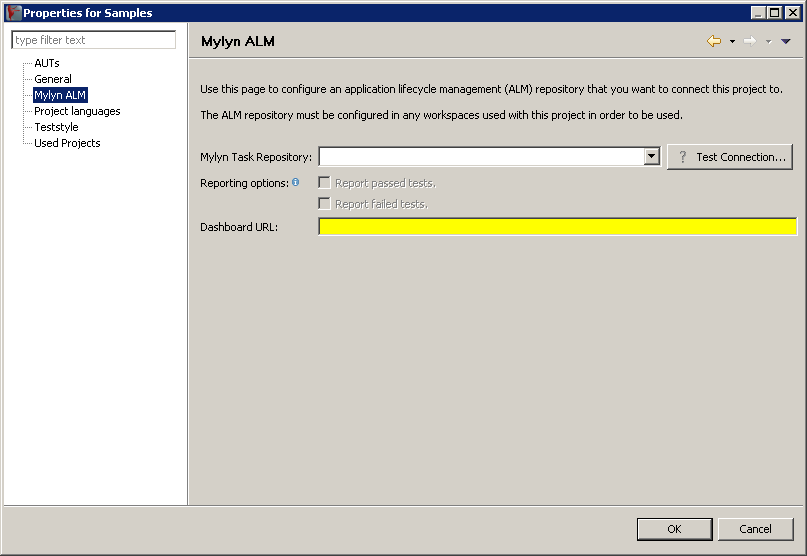
\includegraphics[width=12.5cm]{Tasks/ALM/PS/almproperties}
\caption{ALM Settings}
\label{TasksALMProjectProperties}
\end{center}
\end{figure}


\subsection{Adding task IDs to \gdjobs{}, \gdsuites{} and \gdcases{}}
\label{TasksALMAddTask}
You can add a task ID to \gdcases{}, \gdsuites{} and \gdjobs{} in your \gdproject{}. 

The task ID should be a valid ID in the repository that you have specified as the repository for this \gdproject{} \bxpref{TasksALMConfigureProject}. Adding the task ID to an item in your \gdproject{} means that this item is the relevant test for that task in your repository. When you activate the option, any test results for this item will be added as a comment to the task in the repository. The comment will include a link to the dashboard, in which the test result report can be viewed.

To add a task ID to a \gdcase{}, \gdsuite{} or \gdjob{}:
\begin{enumerate}
\item Open the item in the editor by double-clicking it.
\item In the \gdpropview{}, in the cell for \bxname{Task ID}, enter the task ID from the external repository. You can only enter task IDs at the place of specification -- you cannot overwrite them when you reuse the item.
\item Save the editor. 
\item When you have added a task ID to a node, you can open the task for this node from the browser by selecting:\\
\bxmenu{Open with}{Mylyn Task Editor}{}
\end{enumerate}

\bxtipp{You should ensure that you add task IDs to the right node-level to provide you with the relevant amount of information for the tasks in your repository. This will usually be at the level of Use Cases within a \gdsuite{}. }




\clearpage

\section{Working with test data}
\label{WorkingWithData}
The amount of keywords you have in a \app{} test and the amount of components your test deals with can grow very quickly. For this reason, it is important to think about structuring the \gdtestcasebrowser{} and the \gdomeditor{} to make finding \gdcases{} and component names easier. 


\subsection{Configuring task repositories in your workspace}
\label{TasksALMConfigureWorkspace}
Each repository you want to work with in your \ite{} must be configured in the workspace you are using. 

\begin{enumerate}
\item Select:\\ \bxmenu{Window}{Show View}{Other}\\ from the menu.
\item In the \bxname{Mylyn} section, select \bxname{Task Repositories} and click \bxcaption{OK}. The \bxname{Task Repositories} View will appear. The Bugzilla Repositories for \gd{} and \jb{} are pre-configured.
\item In the \bxname{Task Repositories} View, right click and select \bxname{Add Task Repository} from the context menu.
\item In the dialog that appears, you will see the pre-defined task repositories for the \ite{}. You can select one of these or choose to install a different connector. Depending on the connector you want to use, you may require additional software from Tasktop, or the connector may incur license fees.
\item Once you have selected your connector, click \bxcaption{Next}.
\item On the following page, you will need to configure the task repository. Please refer to the Mylyn documentation for information on repository configuration. 
\item Click \bxcaption{Finish} once the repository is configured.
\item To be able to see tasks in this repository, select: \\ \bxmenu{Window}{Show View}{Other}\\ from the menu. 
\item In the \bxname{Mylyn} section, select \bxname{Task List} and click \bxcaption{OK}. The \bxname{Task List} View will appear.
\end{enumerate}

You will now be able to see items in this repository, open them in the \ite{}, add queries for your workspace and work on tasks from this repository. 
You will also be able to select this repository in the \gdproject{} properties as the repository for your \gdproject{} \bxpref{TasksALMConfigureProject}. 


\subsection{Working on tasks in the \ite{}: contexts}
Once you have configured a task repository for your workspace \bxpref{TasksALMConfigureWorkspace}, you can work on tasks from that repository. 

\subsubsection{Opening and editing tasks in the \ite{}}
\begin{itemize}
\item To be able to see tasks in a repository, select: \\ \bxmenu{Window}{Show View}{Other}\\ from the menu. 
\item In the \bxname{Mylyn} section, select \bxname{Task List} and click \bxcaption{OK}. The \bxname{Task List} View will appear.
\item Double-click on a task to open this task in the editor area.
\item Once a task is open, you can work on it as you would in an external system -- add comments, change status etc.
\end{itemize}

\subsubsection{Working on tasks in the \ite{}}
\label{TasksActivateTask}
Mylyn supports context- or task-based working. When you work on a task, you only see items relevant to that task, so that coming back to the task later involves less context-switching. 
\begin{itemize}
\item Mylyn supports context-based working. You can work on existing tasks in a configured repository, or you can create tasks to work on.
\item To work on a task, you must \bxname{activate} it. To activate a task, select the task in the \bxname{Task List} and select:\\ \bxmenu{Activate}{}{}\\
from the context-sensitive menu. 
\item When you activate a task for the first time, the browsers and editors will seem very empty. This is because nothing is yet a part of the context for this task.
\item You can navigate through the browsers by pressing \bxkey{Alt+Click} to expand each level, or you can press the \bxname{Focus on task} button in the browsers to show the whole tree (not focusing on the task), or just the items in the current context (focusing on the task). 
\item Items are automatically added to your context when you select them in a browser, when you open them in an editor, or when you perform other actions that cause them to be made relevant (e.g. \gdcase{} creation, showing a \gdcase{} specification etc.). Items that are used particularly frequently are marked as \bxname{landmarks} and shown in bold. 
\item You can manually alter which items are in your context using the context-sensitive menu for a specific item. You can manually make items landmarks, or remove them from the context. 
\item The context that is created for you will be re-created when you reactivate the task at a later point. 
\end{itemize}



\subsection{Creating tasks in external repositories from test result reports}
\gdhelpid{testResultViewContextId}{Test Results View}
 You can create a new task with pre-filled information directly from an open test result report in the \gdtestresultview{}. This is useful if a test has failed and you want to create e.g. an issue in your bug-tracking system for the failure. 
\begin{enumerate}
\item In an open test result report, select the node that best describes the test failure (e.g. a \gdcase{} or \gdstep{} that has failed, or the whole \gdsuite{}, then right-click and select:\\
\bxmenu{Create a Mylyn Task}{}{}\\
from the context-sensitive menu.
\item  In the dialog that appears, select a repository in which to create the task. A \bxname{local} repository is available by default, but you can also add connections to Bugzilla and Trac repositories by clicking \bxcaption{Add Task Repository} in the New Task Dialog. Connectors to other repositories can also be added. See the Mylyn documentation for more details on adding repositories.
\item Click \bxcaption{Finish} once you have selected your repository. 
\item The editor for a new task will appear. It is pre-filled with information relevant to the node that you selected. Edit the task to make it descriptive enough for a bug report and save the editor. 
\item Once you have created a task, you can activate it to start saving your context for this task. See the later section \bxpref{TasksActivateTask} for details.
\end{enumerate}


\subsection{Configuring a task repository for your \gdproject{}}
\label{TasksALMConfigureProject}
Once you have configured one or more repositories for your workspace \bxpref{}, you can select one of these to be the test-relevant repository for your \gdproject{}. 

This will let you:
\begin{itemize}
\item Add a task ID from this repository to \gdcases{}, \gdsuites{}, and \gdjobs{} in the \gdproject{} to signify that this item is the test for this task \bxpref{TasksALMAddTask}.
\item Automatically report test results to the task defined when a test runs.
\item View the test results for the relevant item in the dashboard as a link from the task repository.
\end{itemize}

To configure a task repository for your \gdproject{}:

\begin{enumerate}
\item In the \gdproject{} Properties, select \bxname{Mylyn ALM} from the tree on the left \bxfigref{TasksALMProjectProperties}.
\item In the page that appears, you can select a repository from the combo-box.
\item You can then choose whether to only report failed tests, only report successful tests, or both.
\item Enter the URL of the \dash{} that is configured to use the correct \gddb{} for your test results. This is the \dash{} that will be opened when you click on a test result link from the task repository.
\end{enumerate}

\begin{figure}[h]
\begin{center}
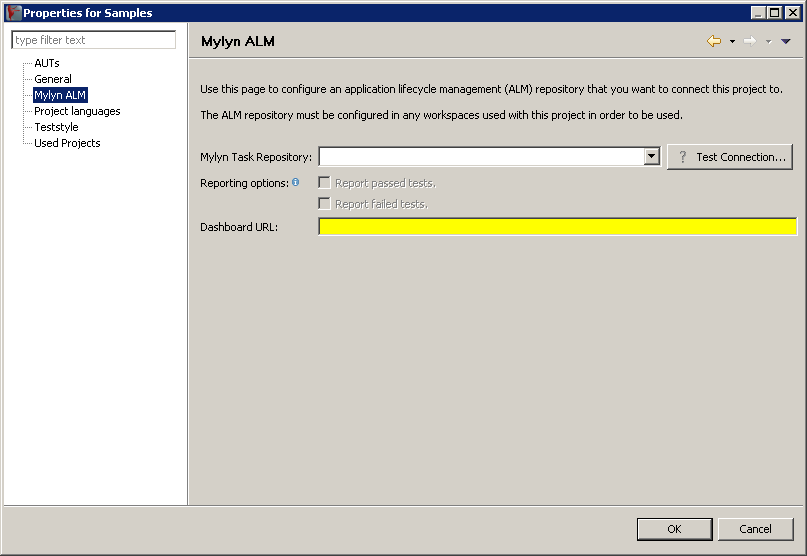
\includegraphics[width=12.5cm]{Tasks/ALM/PS/almproperties}
\caption{ALM Settings}
\label{TasksALMProjectProperties}
\end{center}
\end{figure}


\subsection{Adding task IDs to \gdjobs{}, \gdsuites{} and \gdcases{}}
\label{TasksALMAddTask}
You can add a task ID to \gdcases{}, \gdsuites{} and \gdjobs{} in your \gdproject{}. 

The task ID should be a valid ID in the repository that you have specified as the repository for this \gdproject{} \bxpref{TasksALMConfigureProject}. Adding the task ID to an item in your \gdproject{} means that this item is the relevant test for that task in your repository. When you activate the option, any test results for this item will be added as a comment to the task in the repository. The comment will include a link to the dashboard, in which the test result report can be viewed.

To add a task ID to a \gdcase{}, \gdsuite{} or \gdjob{}:
\begin{enumerate}
\item Open the item in the editor by double-clicking it.
\item In the \gdpropview{}, in the cell for \bxname{Task ID}, enter the task ID from the external repository. You can only enter task IDs at the place of specification -- you cannot overwrite them when you reuse the item.
\item Save the editor. 
\item When you have added a task ID to a node, you can open the task for this node from the browser by selecting:\\
\bxmenu{Open with}{Mylyn Task Editor}{}
\end{enumerate}

\bxtipp{You should ensure that you add task IDs to the right node-level to provide you with the relevant amount of information for the tasks in your repository. This will usually be at the level of Use Cases within a \gdsuite{}. }




\clearpage

\section{Working with component names}
\label{reass}
The amount of keywords you have in a \app{} test and the amount of components your test deals with can grow very quickly. For this reason, it is important to think about structuring the \gdtestcasebrowser{} and the \gdomeditor{} to make finding \gdcases{} and component names easier. 


\subsection{Configuring task repositories in your workspace}
\label{TasksALMConfigureWorkspace}
Each repository you want to work with in your \ite{} must be configured in the workspace you are using. 

\begin{enumerate}
\item Select:\\ \bxmenu{Window}{Show View}{Other}\\ from the menu.
\item In the \bxname{Mylyn} section, select \bxname{Task Repositories} and click \bxcaption{OK}. The \bxname{Task Repositories} View will appear. The Bugzilla Repositories for \gd{} and \jb{} are pre-configured.
\item In the \bxname{Task Repositories} View, right click and select \bxname{Add Task Repository} from the context menu.
\item In the dialog that appears, you will see the pre-defined task repositories for the \ite{}. You can select one of these or choose to install a different connector. Depending on the connector you want to use, you may require additional software from Tasktop, or the connector may incur license fees.
\item Once you have selected your connector, click \bxcaption{Next}.
\item On the following page, you will need to configure the task repository. Please refer to the Mylyn documentation for information on repository configuration. 
\item Click \bxcaption{Finish} once the repository is configured.
\item To be able to see tasks in this repository, select: \\ \bxmenu{Window}{Show View}{Other}\\ from the menu. 
\item In the \bxname{Mylyn} section, select \bxname{Task List} and click \bxcaption{OK}. The \bxname{Task List} View will appear.
\end{enumerate}

You will now be able to see items in this repository, open them in the \ite{}, add queries for your workspace and work on tasks from this repository. 
You will also be able to select this repository in the \gdproject{} properties as the repository for your \gdproject{} \bxpref{TasksALMConfigureProject}. 


\subsection{Working on tasks in the \ite{}: contexts}
Once you have configured a task repository for your workspace \bxpref{TasksALMConfigureWorkspace}, you can work on tasks from that repository. 

\subsubsection{Opening and editing tasks in the \ite{}}
\begin{itemize}
\item To be able to see tasks in a repository, select: \\ \bxmenu{Window}{Show View}{Other}\\ from the menu. 
\item In the \bxname{Mylyn} section, select \bxname{Task List} and click \bxcaption{OK}. The \bxname{Task List} View will appear.
\item Double-click on a task to open this task in the editor area.
\item Once a task is open, you can work on it as you would in an external system -- add comments, change status etc.
\end{itemize}

\subsubsection{Working on tasks in the \ite{}}
\label{TasksActivateTask}
Mylyn supports context- or task-based working. When you work on a task, you only see items relevant to that task, so that coming back to the task later involves less context-switching. 
\begin{itemize}
\item Mylyn supports context-based working. You can work on existing tasks in a configured repository, or you can create tasks to work on.
\item To work on a task, you must \bxname{activate} it. To activate a task, select the task in the \bxname{Task List} and select:\\ \bxmenu{Activate}{}{}\\
from the context-sensitive menu. 
\item When you activate a task for the first time, the browsers and editors will seem very empty. This is because nothing is yet a part of the context for this task.
\item You can navigate through the browsers by pressing \bxkey{Alt+Click} to expand each level, or you can press the \bxname{Focus on task} button in the browsers to show the whole tree (not focusing on the task), or just the items in the current context (focusing on the task). 
\item Items are automatically added to your context when you select them in a browser, when you open them in an editor, or when you perform other actions that cause them to be made relevant (e.g. \gdcase{} creation, showing a \gdcase{} specification etc.). Items that are used particularly frequently are marked as \bxname{landmarks} and shown in bold. 
\item You can manually alter which items are in your context using the context-sensitive menu for a specific item. You can manually make items landmarks, or remove them from the context. 
\item The context that is created for you will be re-created when you reactivate the task at a later point. 
\end{itemize}



\subsection{Creating tasks in external repositories from test result reports}
\gdhelpid{testResultViewContextId}{Test Results View}
 You can create a new task with pre-filled information directly from an open test result report in the \gdtestresultview{}. This is useful if a test has failed and you want to create e.g. an issue in your bug-tracking system for the failure. 
\begin{enumerate}
\item In an open test result report, select the node that best describes the test failure (e.g. a \gdcase{} or \gdstep{} that has failed, or the whole \gdsuite{}, then right-click and select:\\
\bxmenu{Create a Mylyn Task}{}{}\\
from the context-sensitive menu.
\item  In the dialog that appears, select a repository in which to create the task. A \bxname{local} repository is available by default, but you can also add connections to Bugzilla and Trac repositories by clicking \bxcaption{Add Task Repository} in the New Task Dialog. Connectors to other repositories can also be added. See the Mylyn documentation for more details on adding repositories.
\item Click \bxcaption{Finish} once you have selected your repository. 
\item The editor for a new task will appear. It is pre-filled with information relevant to the node that you selected. Edit the task to make it descriptive enough for a bug report and save the editor. 
\item Once you have created a task, you can activate it to start saving your context for this task. See the later section \bxpref{TasksActivateTask} for details.
\end{enumerate}


\subsection{Configuring a task repository for your \gdproject{}}
\label{TasksALMConfigureProject}
Once you have configured one or more repositories for your workspace \bxpref{}, you can select one of these to be the test-relevant repository for your \gdproject{}. 

This will let you:
\begin{itemize}
\item Add a task ID from this repository to \gdcases{}, \gdsuites{}, and \gdjobs{} in the \gdproject{} to signify that this item is the test for this task \bxpref{TasksALMAddTask}.
\item Automatically report test results to the task defined when a test runs.
\item View the test results for the relevant item in the dashboard as a link from the task repository.
\end{itemize}

To configure a task repository for your \gdproject{}:

\begin{enumerate}
\item In the \gdproject{} Properties, select \bxname{Mylyn ALM} from the tree on the left \bxfigref{TasksALMProjectProperties}.
\item In the page that appears, you can select a repository from the combo-box.
\item You can then choose whether to only report failed tests, only report successful tests, or both.
\item Enter the URL of the \dash{} that is configured to use the correct \gddb{} for your test results. This is the \dash{} that will be opened when you click on a test result link from the task repository.
\end{enumerate}

\begin{figure}[h]
\begin{center}
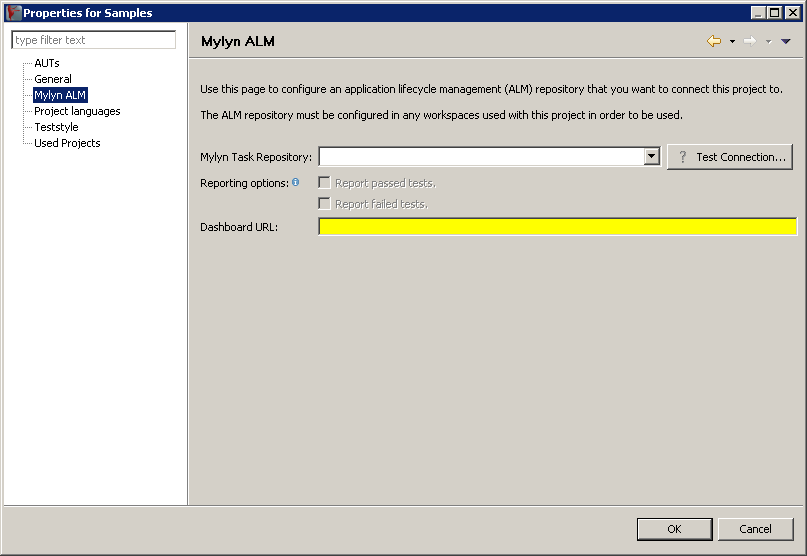
\includegraphics[width=12.5cm]{Tasks/ALM/PS/almproperties}
\caption{ALM Settings}
\label{TasksALMProjectProperties}
\end{center}
\end{figure}


\subsection{Adding task IDs to \gdjobs{}, \gdsuites{} and \gdcases{}}
\label{TasksALMAddTask}
You can add a task ID to \gdcases{}, \gdsuites{} and \gdjobs{} in your \gdproject{}. 

The task ID should be a valid ID in the repository that you have specified as the repository for this \gdproject{} \bxpref{TasksALMConfigureProject}. Adding the task ID to an item in your \gdproject{} means that this item is the relevant test for that task in your repository. When you activate the option, any test results for this item will be added as a comment to the task in the repository. The comment will include a link to the dashboard, in which the test result report can be viewed.

To add a task ID to a \gdcase{}, \gdsuite{} or \gdjob{}:
\begin{enumerate}
\item Open the item in the editor by double-clicking it.
\item In the \gdpropview{}, in the cell for \bxname{Task ID}, enter the task ID from the external repository. You can only enter task IDs at the place of specification -- you cannot overwrite them when you reuse the item.
\item Save the editor. 
\item When you have added a task ID to a node, you can open the task for this node from the browser by selecting:\\
\bxmenu{Open with}{Mylyn Task Editor}{}
\end{enumerate}

\bxtipp{You should ensure that you add task IDs to the right node-level to provide you with the relevant amount of information for the tasks in your repository. This will usually be at the level of Use Cases within a \gdsuite{}. }





\clearpage

\section{Working with \gdsuites{}}
\label{WorkingWithSuites}
The amount of keywords you have in a \app{} test and the amount of components your test deals with can grow very quickly. For this reason, it is important to think about structuring the \gdtestcasebrowser{} and the \gdomeditor{} to make finding \gdcases{} and component names easier. 


\subsection{Configuring task repositories in your workspace}
\label{TasksALMConfigureWorkspace}
Each repository you want to work with in your \ite{} must be configured in the workspace you are using. 

\begin{enumerate}
\item Select:\\ \bxmenu{Window}{Show View}{Other}\\ from the menu.
\item In the \bxname{Mylyn} section, select \bxname{Task Repositories} and click \bxcaption{OK}. The \bxname{Task Repositories} View will appear. The Bugzilla Repositories for \gd{} and \jb{} are pre-configured.
\item In the \bxname{Task Repositories} View, right click and select \bxname{Add Task Repository} from the context menu.
\item In the dialog that appears, you will see the pre-defined task repositories for the \ite{}. You can select one of these or choose to install a different connector. Depending on the connector you want to use, you may require additional software from Tasktop, or the connector may incur license fees.
\item Once you have selected your connector, click \bxcaption{Next}.
\item On the following page, you will need to configure the task repository. Please refer to the Mylyn documentation for information on repository configuration. 
\item Click \bxcaption{Finish} once the repository is configured.
\item To be able to see tasks in this repository, select: \\ \bxmenu{Window}{Show View}{Other}\\ from the menu. 
\item In the \bxname{Mylyn} section, select \bxname{Task List} and click \bxcaption{OK}. The \bxname{Task List} View will appear.
\end{enumerate}

You will now be able to see items in this repository, open them in the \ite{}, add queries for your workspace and work on tasks from this repository. 
You will also be able to select this repository in the \gdproject{} properties as the repository for your \gdproject{} \bxpref{TasksALMConfigureProject}. 


\subsection{Working on tasks in the \ite{}: contexts}
Once you have configured a task repository for your workspace \bxpref{TasksALMConfigureWorkspace}, you can work on tasks from that repository. 

\subsubsection{Opening and editing tasks in the \ite{}}
\begin{itemize}
\item To be able to see tasks in a repository, select: \\ \bxmenu{Window}{Show View}{Other}\\ from the menu. 
\item In the \bxname{Mylyn} section, select \bxname{Task List} and click \bxcaption{OK}. The \bxname{Task List} View will appear.
\item Double-click on a task to open this task in the editor area.
\item Once a task is open, you can work on it as you would in an external system -- add comments, change status etc.
\end{itemize}

\subsubsection{Working on tasks in the \ite{}}
\label{TasksActivateTask}
Mylyn supports context- or task-based working. When you work on a task, you only see items relevant to that task, so that coming back to the task later involves less context-switching. 
\begin{itemize}
\item Mylyn supports context-based working. You can work on existing tasks in a configured repository, or you can create tasks to work on.
\item To work on a task, you must \bxname{activate} it. To activate a task, select the task in the \bxname{Task List} and select:\\ \bxmenu{Activate}{}{}\\
from the context-sensitive menu. 
\item When you activate a task for the first time, the browsers and editors will seem very empty. This is because nothing is yet a part of the context for this task.
\item You can navigate through the browsers by pressing \bxkey{Alt+Click} to expand each level, or you can press the \bxname{Focus on task} button in the browsers to show the whole tree (not focusing on the task), or just the items in the current context (focusing on the task). 
\item Items are automatically added to your context when you select them in a browser, when you open them in an editor, or when you perform other actions that cause them to be made relevant (e.g. \gdcase{} creation, showing a \gdcase{} specification etc.). Items that are used particularly frequently are marked as \bxname{landmarks} and shown in bold. 
\item You can manually alter which items are in your context using the context-sensitive menu for a specific item. You can manually make items landmarks, or remove them from the context. 
\item The context that is created for you will be re-created when you reactivate the task at a later point. 
\end{itemize}



\subsection{Creating tasks in external repositories from test result reports}
\gdhelpid{testResultViewContextId}{Test Results View}
 You can create a new task with pre-filled information directly from an open test result report in the \gdtestresultview{}. This is useful if a test has failed and you want to create e.g. an issue in your bug-tracking system for the failure. 
\begin{enumerate}
\item In an open test result report, select the node that best describes the test failure (e.g. a \gdcase{} or \gdstep{} that has failed, or the whole \gdsuite{}, then right-click and select:\\
\bxmenu{Create a Mylyn Task}{}{}\\
from the context-sensitive menu.
\item  In the dialog that appears, select a repository in which to create the task. A \bxname{local} repository is available by default, but you can also add connections to Bugzilla and Trac repositories by clicking \bxcaption{Add Task Repository} in the New Task Dialog. Connectors to other repositories can also be added. See the Mylyn documentation for more details on adding repositories.
\item Click \bxcaption{Finish} once you have selected your repository. 
\item The editor for a new task will appear. It is pre-filled with information relevant to the node that you selected. Edit the task to make it descriptive enough for a bug report and save the editor. 
\item Once you have created a task, you can activate it to start saving your context for this task. See the later section \bxpref{TasksActivateTask} for details.
\end{enumerate}


\subsection{Configuring a task repository for your \gdproject{}}
\label{TasksALMConfigureProject}
Once you have configured one or more repositories for your workspace \bxpref{}, you can select one of these to be the test-relevant repository for your \gdproject{}. 

This will let you:
\begin{itemize}
\item Add a task ID from this repository to \gdcases{}, \gdsuites{}, and \gdjobs{} in the \gdproject{} to signify that this item is the test for this task \bxpref{TasksALMAddTask}.
\item Automatically report test results to the task defined when a test runs.
\item View the test results for the relevant item in the dashboard as a link from the task repository.
\end{itemize}

To configure a task repository for your \gdproject{}:

\begin{enumerate}
\item In the \gdproject{} Properties, select \bxname{Mylyn ALM} from the tree on the left \bxfigref{TasksALMProjectProperties}.
\item In the page that appears, you can select a repository from the combo-box.
\item You can then choose whether to only report failed tests, only report successful tests, or both.
\item Enter the URL of the \dash{} that is configured to use the correct \gddb{} for your test results. This is the \dash{} that will be opened when you click on a test result link from the task repository.
\end{enumerate}

\begin{figure}[h]
\begin{center}
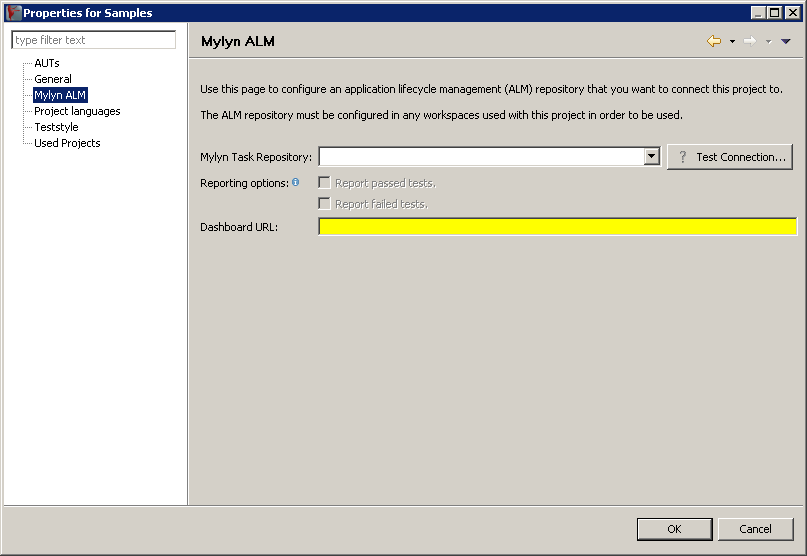
\includegraphics[width=12.5cm]{Tasks/ALM/PS/almproperties}
\caption{ALM Settings}
\label{TasksALMProjectProperties}
\end{center}
\end{figure}


\subsection{Adding task IDs to \gdjobs{}, \gdsuites{} and \gdcases{}}
\label{TasksALMAddTask}
You can add a task ID to \gdcases{}, \gdsuites{} and \gdjobs{} in your \gdproject{}. 

The task ID should be a valid ID in the repository that you have specified as the repository for this \gdproject{} \bxpref{TasksALMConfigureProject}. Adding the task ID to an item in your \gdproject{} means that this item is the relevant test for that task in your repository. When you activate the option, any test results for this item will be added as a comment to the task in the repository. The comment will include a link to the dashboard, in which the test result report can be viewed.

To add a task ID to a \gdcase{}, \gdsuite{} or \gdjob{}:
\begin{enumerate}
\item Open the item in the editor by double-clicking it.
\item In the \gdpropview{}, in the cell for \bxname{Task ID}, enter the task ID from the external repository. You can only enter task IDs at the place of specification -- you cannot overwrite them when you reuse the item.
\item Save the editor. 
\item When you have added a task ID to a node, you can open the task for this node from the browser by selecting:\\
\bxmenu{Open with}{Mylyn Task Editor}{}
\end{enumerate}

\bxtipp{You should ensure that you add task IDs to the right node-level to provide you with the relevant amount of information for the tasks in your repository. This will usually be at the level of Use Cases within a \gdsuite{}. }




\clearpage 

\section{Working with \gdjobs{} to test multiple \gdauts{}}
\label{WorkingWithJobs}
The amount of keywords you have in a \app{} test and the amount of components your test deals with can grow very quickly. For this reason, it is important to think about structuring the \gdtestcasebrowser{} and the \gdomeditor{} to make finding \gdcases{} and component names easier. 


\subsection{Configuring task repositories in your workspace}
\label{TasksALMConfigureWorkspace}
Each repository you want to work with in your \ite{} must be configured in the workspace you are using. 

\begin{enumerate}
\item Select:\\ \bxmenu{Window}{Show View}{Other}\\ from the menu.
\item In the \bxname{Mylyn} section, select \bxname{Task Repositories} and click \bxcaption{OK}. The \bxname{Task Repositories} View will appear. The Bugzilla Repositories for \gd{} and \jb{} are pre-configured.
\item In the \bxname{Task Repositories} View, right click and select \bxname{Add Task Repository} from the context menu.
\item In the dialog that appears, you will see the pre-defined task repositories for the \ite{}. You can select one of these or choose to install a different connector. Depending on the connector you want to use, you may require additional software from Tasktop, or the connector may incur license fees.
\item Once you have selected your connector, click \bxcaption{Next}.
\item On the following page, you will need to configure the task repository. Please refer to the Mylyn documentation for information on repository configuration. 
\item Click \bxcaption{Finish} once the repository is configured.
\item To be able to see tasks in this repository, select: \\ \bxmenu{Window}{Show View}{Other}\\ from the menu. 
\item In the \bxname{Mylyn} section, select \bxname{Task List} and click \bxcaption{OK}. The \bxname{Task List} View will appear.
\end{enumerate}

You will now be able to see items in this repository, open them in the \ite{}, add queries for your workspace and work on tasks from this repository. 
You will also be able to select this repository in the \gdproject{} properties as the repository for your \gdproject{} \bxpref{TasksALMConfigureProject}. 


\subsection{Working on tasks in the \ite{}: contexts}
Once you have configured a task repository for your workspace \bxpref{TasksALMConfigureWorkspace}, you can work on tasks from that repository. 

\subsubsection{Opening and editing tasks in the \ite{}}
\begin{itemize}
\item To be able to see tasks in a repository, select: \\ \bxmenu{Window}{Show View}{Other}\\ from the menu. 
\item In the \bxname{Mylyn} section, select \bxname{Task List} and click \bxcaption{OK}. The \bxname{Task List} View will appear.
\item Double-click on a task to open this task in the editor area.
\item Once a task is open, you can work on it as you would in an external system -- add comments, change status etc.
\end{itemize}

\subsubsection{Working on tasks in the \ite{}}
\label{TasksActivateTask}
Mylyn supports context- or task-based working. When you work on a task, you only see items relevant to that task, so that coming back to the task later involves less context-switching. 
\begin{itemize}
\item Mylyn supports context-based working. You can work on existing tasks in a configured repository, or you can create tasks to work on.
\item To work on a task, you must \bxname{activate} it. To activate a task, select the task in the \bxname{Task List} and select:\\ \bxmenu{Activate}{}{}\\
from the context-sensitive menu. 
\item When you activate a task for the first time, the browsers and editors will seem very empty. This is because nothing is yet a part of the context for this task.
\item You can navigate through the browsers by pressing \bxkey{Alt+Click} to expand each level, or you can press the \bxname{Focus on task} button in the browsers to show the whole tree (not focusing on the task), or just the items in the current context (focusing on the task). 
\item Items are automatically added to your context when you select them in a browser, when you open them in an editor, or when you perform other actions that cause them to be made relevant (e.g. \gdcase{} creation, showing a \gdcase{} specification etc.). Items that are used particularly frequently are marked as \bxname{landmarks} and shown in bold. 
\item You can manually alter which items are in your context using the context-sensitive menu for a specific item. You can manually make items landmarks, or remove them from the context. 
\item The context that is created for you will be re-created when you reactivate the task at a later point. 
\end{itemize}



\subsection{Creating tasks in external repositories from test result reports}
\gdhelpid{testResultViewContextId}{Test Results View}
 You can create a new task with pre-filled information directly from an open test result report in the \gdtestresultview{}. This is useful if a test has failed and you want to create e.g. an issue in your bug-tracking system for the failure. 
\begin{enumerate}
\item In an open test result report, select the node that best describes the test failure (e.g. a \gdcase{} or \gdstep{} that has failed, or the whole \gdsuite{}, then right-click and select:\\
\bxmenu{Create a Mylyn Task}{}{}\\
from the context-sensitive menu.
\item  In the dialog that appears, select a repository in which to create the task. A \bxname{local} repository is available by default, but you can also add connections to Bugzilla and Trac repositories by clicking \bxcaption{Add Task Repository} in the New Task Dialog. Connectors to other repositories can also be added. See the Mylyn documentation for more details on adding repositories.
\item Click \bxcaption{Finish} once you have selected your repository. 
\item The editor for a new task will appear. It is pre-filled with information relevant to the node that you selected. Edit the task to make it descriptive enough for a bug report and save the editor. 
\item Once you have created a task, you can activate it to start saving your context for this task. See the later section \bxpref{TasksActivateTask} for details.
\end{enumerate}


\subsection{Configuring a task repository for your \gdproject{}}
\label{TasksALMConfigureProject}
Once you have configured one or more repositories for your workspace \bxpref{}, you can select one of these to be the test-relevant repository for your \gdproject{}. 

This will let you:
\begin{itemize}
\item Add a task ID from this repository to \gdcases{}, \gdsuites{}, and \gdjobs{} in the \gdproject{} to signify that this item is the test for this task \bxpref{TasksALMAddTask}.
\item Automatically report test results to the task defined when a test runs.
\item View the test results for the relevant item in the dashboard as a link from the task repository.
\end{itemize}

To configure a task repository for your \gdproject{}:

\begin{enumerate}
\item In the \gdproject{} Properties, select \bxname{Mylyn ALM} from the tree on the left \bxfigref{TasksALMProjectProperties}.
\item In the page that appears, you can select a repository from the combo-box.
\item You can then choose whether to only report failed tests, only report successful tests, or both.
\item Enter the URL of the \dash{} that is configured to use the correct \gddb{} for your test results. This is the \dash{} that will be opened when you click on a test result link from the task repository.
\end{enumerate}

\begin{figure}[h]
\begin{center}
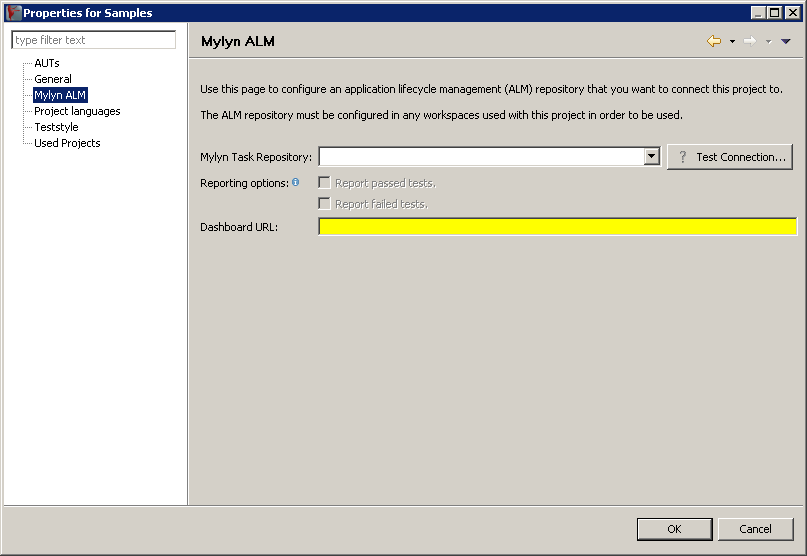
\includegraphics[width=12.5cm]{Tasks/ALM/PS/almproperties}
\caption{ALM Settings}
\label{TasksALMProjectProperties}
\end{center}
\end{figure}


\subsection{Adding task IDs to \gdjobs{}, \gdsuites{} and \gdcases{}}
\label{TasksALMAddTask}
You can add a task ID to \gdcases{}, \gdsuites{} and \gdjobs{} in your \gdproject{}. 

The task ID should be a valid ID in the repository that you have specified as the repository for this \gdproject{} \bxpref{TasksALMConfigureProject}. Adding the task ID to an item in your \gdproject{} means that this item is the relevant test for that task in your repository. When you activate the option, any test results for this item will be added as a comment to the task in the repository. The comment will include a link to the dashboard, in which the test result report can be viewed.

To add a task ID to a \gdcase{}, \gdsuite{} or \gdjob{}:
\begin{enumerate}
\item Open the item in the editor by double-clicking it.
\item In the \gdpropview{}, in the cell for \bxname{Task ID}, enter the task ID from the external repository. You can only enter task IDs at the place of specification -- you cannot overwrite them when you reuse the item.
\item Save the editor. 
\item When you have added a task ID to a node, you can open the task for this node from the browser by selecting:\\
\bxmenu{Open with}{Mylyn Task Editor}{}
\end{enumerate}

\bxtipp{You should ensure that you add task IDs to the right node-level to provide you with the relevant amount of information for the tasks in your repository. This will usually be at the level of Use Cases within a \gdsuite{}. }




\clearpage 

\section{Information on \gdsteps{}}
\gdhelpid{capContextId}{Test Steps}
The amount of keywords you have in a \app{} test and the amount of components your test deals with can grow very quickly. For this reason, it is important to think about structuring the \gdtestcasebrowser{} and the \gdomeditor{} to make finding \gdcases{} and component names easier. 


\subsection{Configuring task repositories in your workspace}
\label{TasksALMConfigureWorkspace}
Each repository you want to work with in your \ite{} must be configured in the workspace you are using. 

\begin{enumerate}
\item Select:\\ \bxmenu{Window}{Show View}{Other}\\ from the menu.
\item In the \bxname{Mylyn} section, select \bxname{Task Repositories} and click \bxcaption{OK}. The \bxname{Task Repositories} View will appear. The Bugzilla Repositories for \gd{} and \jb{} are pre-configured.
\item In the \bxname{Task Repositories} View, right click and select \bxname{Add Task Repository} from the context menu.
\item In the dialog that appears, you will see the pre-defined task repositories for the \ite{}. You can select one of these or choose to install a different connector. Depending on the connector you want to use, you may require additional software from Tasktop, or the connector may incur license fees.
\item Once you have selected your connector, click \bxcaption{Next}.
\item On the following page, you will need to configure the task repository. Please refer to the Mylyn documentation for information on repository configuration. 
\item Click \bxcaption{Finish} once the repository is configured.
\item To be able to see tasks in this repository, select: \\ \bxmenu{Window}{Show View}{Other}\\ from the menu. 
\item In the \bxname{Mylyn} section, select \bxname{Task List} and click \bxcaption{OK}. The \bxname{Task List} View will appear.
\end{enumerate}

You will now be able to see items in this repository, open them in the \ite{}, add queries for your workspace and work on tasks from this repository. 
You will also be able to select this repository in the \gdproject{} properties as the repository for your \gdproject{} \bxpref{TasksALMConfigureProject}. 


\subsection{Working on tasks in the \ite{}: contexts}
Once you have configured a task repository for your workspace \bxpref{TasksALMConfigureWorkspace}, you can work on tasks from that repository. 

\subsubsection{Opening and editing tasks in the \ite{}}
\begin{itemize}
\item To be able to see tasks in a repository, select: \\ \bxmenu{Window}{Show View}{Other}\\ from the menu. 
\item In the \bxname{Mylyn} section, select \bxname{Task List} and click \bxcaption{OK}. The \bxname{Task List} View will appear.
\item Double-click on a task to open this task in the editor area.
\item Once a task is open, you can work on it as you would in an external system -- add comments, change status etc.
\end{itemize}

\subsubsection{Working on tasks in the \ite{}}
\label{TasksActivateTask}
Mylyn supports context- or task-based working. When you work on a task, you only see items relevant to that task, so that coming back to the task later involves less context-switching. 
\begin{itemize}
\item Mylyn supports context-based working. You can work on existing tasks in a configured repository, or you can create tasks to work on.
\item To work on a task, you must \bxname{activate} it. To activate a task, select the task in the \bxname{Task List} and select:\\ \bxmenu{Activate}{}{}\\
from the context-sensitive menu. 
\item When you activate a task for the first time, the browsers and editors will seem very empty. This is because nothing is yet a part of the context for this task.
\item You can navigate through the browsers by pressing \bxkey{Alt+Click} to expand each level, or you can press the \bxname{Focus on task} button in the browsers to show the whole tree (not focusing on the task), or just the items in the current context (focusing on the task). 
\item Items are automatically added to your context when you select them in a browser, when you open them in an editor, or when you perform other actions that cause them to be made relevant (e.g. \gdcase{} creation, showing a \gdcase{} specification etc.). Items that are used particularly frequently are marked as \bxname{landmarks} and shown in bold. 
\item You can manually alter which items are in your context using the context-sensitive menu for a specific item. You can manually make items landmarks, or remove them from the context. 
\item The context that is created for you will be re-created when you reactivate the task at a later point. 
\end{itemize}



\subsection{Creating tasks in external repositories from test result reports}
\gdhelpid{testResultViewContextId}{Test Results View}
 You can create a new task with pre-filled information directly from an open test result report in the \gdtestresultview{}. This is useful if a test has failed and you want to create e.g. an issue in your bug-tracking system for the failure. 
\begin{enumerate}
\item In an open test result report, select the node that best describes the test failure (e.g. a \gdcase{} or \gdstep{} that has failed, or the whole \gdsuite{}, then right-click and select:\\
\bxmenu{Create a Mylyn Task}{}{}\\
from the context-sensitive menu.
\item  In the dialog that appears, select a repository in which to create the task. A \bxname{local} repository is available by default, but you can also add connections to Bugzilla and Trac repositories by clicking \bxcaption{Add Task Repository} in the New Task Dialog. Connectors to other repositories can also be added. See the Mylyn documentation for more details on adding repositories.
\item Click \bxcaption{Finish} once you have selected your repository. 
\item The editor for a new task will appear. It is pre-filled with information relevant to the node that you selected. Edit the task to make it descriptive enough for a bug report and save the editor. 
\item Once you have created a task, you can activate it to start saving your context for this task. See the later section \bxpref{TasksActivateTask} for details.
\end{enumerate}


\subsection{Configuring a task repository for your \gdproject{}}
\label{TasksALMConfigureProject}
Once you have configured one or more repositories for your workspace \bxpref{}, you can select one of these to be the test-relevant repository for your \gdproject{}. 

This will let you:
\begin{itemize}
\item Add a task ID from this repository to \gdcases{}, \gdsuites{}, and \gdjobs{} in the \gdproject{} to signify that this item is the test for this task \bxpref{TasksALMAddTask}.
\item Automatically report test results to the task defined when a test runs.
\item View the test results for the relevant item in the dashboard as a link from the task repository.
\end{itemize}

To configure a task repository for your \gdproject{}:

\begin{enumerate}
\item In the \gdproject{} Properties, select \bxname{Mylyn ALM} from the tree on the left \bxfigref{TasksALMProjectProperties}.
\item In the page that appears, you can select a repository from the combo-box.
\item You can then choose whether to only report failed tests, only report successful tests, or both.
\item Enter the URL of the \dash{} that is configured to use the correct \gddb{} for your test results. This is the \dash{} that will be opened when you click on a test result link from the task repository.
\end{enumerate}

\begin{figure}[h]
\begin{center}
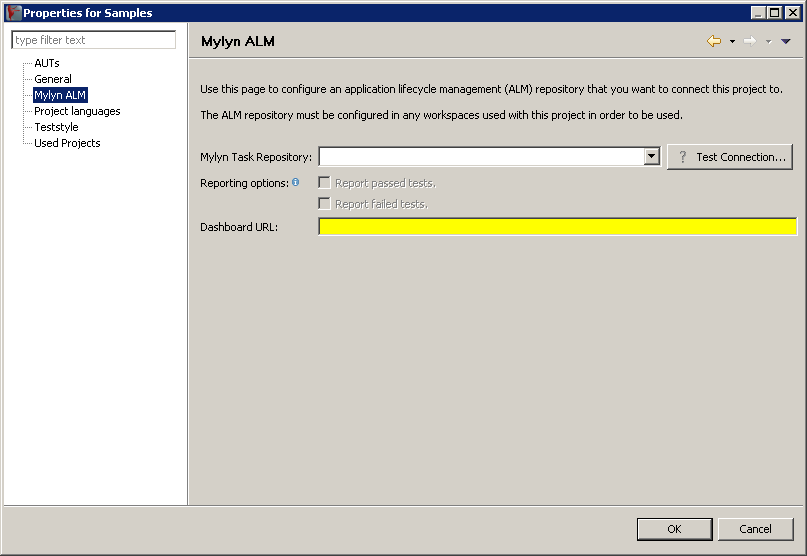
\includegraphics[width=12.5cm]{Tasks/ALM/PS/almproperties}
\caption{ALM Settings}
\label{TasksALMProjectProperties}
\end{center}
\end{figure}


\subsection{Adding task IDs to \gdjobs{}, \gdsuites{} and \gdcases{}}
\label{TasksALMAddTask}
You can add a task ID to \gdcases{}, \gdsuites{} and \gdjobs{} in your \gdproject{}. 

The task ID should be a valid ID in the repository that you have specified as the repository for this \gdproject{} \bxpref{TasksALMConfigureProject}. Adding the task ID to an item in your \gdproject{} means that this item is the relevant test for that task in your repository. When you activate the option, any test results for this item will be added as a comment to the task in the repository. The comment will include a link to the dashboard, in which the test result report can be viewed.

To add a task ID to a \gdcase{}, \gdsuite{} or \gdjob{}:
\begin{enumerate}
\item Open the item in the editor by double-clicking it.
\item In the \gdpropview{}, in the cell for \bxname{Task ID}, enter the task ID from the external repository. You can only enter task IDs at the place of specification -- you cannot overwrite them when you reuse the item.
\item Save the editor. 
\item When you have added a task ID to a node, you can open the task for this node from the browser by selecting:\\
\bxmenu{Open with}{Mylyn Task Editor}{}
\end{enumerate}

\bxtipp{You should ensure that you add task IDs to the right node-level to provide you with the relevant amount of information for the tasks in your repository. This will usually be at the level of Use Cases within a \gdsuite{}. }




\section{Working with manual \gdcases{}}
The amount of keywords you have in a \app{} test and the amount of components your test deals with can grow very quickly. For this reason, it is important to think about structuring the \gdtestcasebrowser{} and the \gdomeditor{} to make finding \gdcases{} and component names easier. 


\subsection{Configuring task repositories in your workspace}
\label{TasksALMConfigureWorkspace}
Each repository you want to work with in your \ite{} must be configured in the workspace you are using. 

\begin{enumerate}
\item Select:\\ \bxmenu{Window}{Show View}{Other}\\ from the menu.
\item In the \bxname{Mylyn} section, select \bxname{Task Repositories} and click \bxcaption{OK}. The \bxname{Task Repositories} View will appear. The Bugzilla Repositories for \gd{} and \jb{} are pre-configured.
\item In the \bxname{Task Repositories} View, right click and select \bxname{Add Task Repository} from the context menu.
\item In the dialog that appears, you will see the pre-defined task repositories for the \ite{}. You can select one of these or choose to install a different connector. Depending on the connector you want to use, you may require additional software from Tasktop, or the connector may incur license fees.
\item Once you have selected your connector, click \bxcaption{Next}.
\item On the following page, you will need to configure the task repository. Please refer to the Mylyn documentation for information on repository configuration. 
\item Click \bxcaption{Finish} once the repository is configured.
\item To be able to see tasks in this repository, select: \\ \bxmenu{Window}{Show View}{Other}\\ from the menu. 
\item In the \bxname{Mylyn} section, select \bxname{Task List} and click \bxcaption{OK}. The \bxname{Task List} View will appear.
\end{enumerate}

You will now be able to see items in this repository, open them in the \ite{}, add queries for your workspace and work on tasks from this repository. 
You will also be able to select this repository in the \gdproject{} properties as the repository for your \gdproject{} \bxpref{TasksALMConfigureProject}. 


\subsection{Working on tasks in the \ite{}: contexts}
Once you have configured a task repository for your workspace \bxpref{TasksALMConfigureWorkspace}, you can work on tasks from that repository. 

\subsubsection{Opening and editing tasks in the \ite{}}
\begin{itemize}
\item To be able to see tasks in a repository, select: \\ \bxmenu{Window}{Show View}{Other}\\ from the menu. 
\item In the \bxname{Mylyn} section, select \bxname{Task List} and click \bxcaption{OK}. The \bxname{Task List} View will appear.
\item Double-click on a task to open this task in the editor area.
\item Once a task is open, you can work on it as you would in an external system -- add comments, change status etc.
\end{itemize}

\subsubsection{Working on tasks in the \ite{}}
\label{TasksActivateTask}
Mylyn supports context- or task-based working. When you work on a task, you only see items relevant to that task, so that coming back to the task later involves less context-switching. 
\begin{itemize}
\item Mylyn supports context-based working. You can work on existing tasks in a configured repository, or you can create tasks to work on.
\item To work on a task, you must \bxname{activate} it. To activate a task, select the task in the \bxname{Task List} and select:\\ \bxmenu{Activate}{}{}\\
from the context-sensitive menu. 
\item When you activate a task for the first time, the browsers and editors will seem very empty. This is because nothing is yet a part of the context for this task.
\item You can navigate through the browsers by pressing \bxkey{Alt+Click} to expand each level, or you can press the \bxname{Focus on task} button in the browsers to show the whole tree (not focusing on the task), or just the items in the current context (focusing on the task). 
\item Items are automatically added to your context when you select them in a browser, when you open them in an editor, or when you perform other actions that cause them to be made relevant (e.g. \gdcase{} creation, showing a \gdcase{} specification etc.). Items that are used particularly frequently are marked as \bxname{landmarks} and shown in bold. 
\item You can manually alter which items are in your context using the context-sensitive menu for a specific item. You can manually make items landmarks, or remove them from the context. 
\item The context that is created for you will be re-created when you reactivate the task at a later point. 
\end{itemize}



\subsection{Creating tasks in external repositories from test result reports}
\gdhelpid{testResultViewContextId}{Test Results View}
 You can create a new task with pre-filled information directly from an open test result report in the \gdtestresultview{}. This is useful if a test has failed and you want to create e.g. an issue in your bug-tracking system for the failure. 
\begin{enumerate}
\item In an open test result report, select the node that best describes the test failure (e.g. a \gdcase{} or \gdstep{} that has failed, or the whole \gdsuite{}, then right-click and select:\\
\bxmenu{Create a Mylyn Task}{}{}\\
from the context-sensitive menu.
\item  In the dialog that appears, select a repository in which to create the task. A \bxname{local} repository is available by default, but you can also add connections to Bugzilla and Trac repositories by clicking \bxcaption{Add Task Repository} in the New Task Dialog. Connectors to other repositories can also be added. See the Mylyn documentation for more details on adding repositories.
\item Click \bxcaption{Finish} once you have selected your repository. 
\item The editor for a new task will appear. It is pre-filled with information relevant to the node that you selected. Edit the task to make it descriptive enough for a bug report and save the editor. 
\item Once you have created a task, you can activate it to start saving your context for this task. See the later section \bxpref{TasksActivateTask} for details.
\end{enumerate}


\subsection{Configuring a task repository for your \gdproject{}}
\label{TasksALMConfigureProject}
Once you have configured one or more repositories for your workspace \bxpref{}, you can select one of these to be the test-relevant repository for your \gdproject{}. 

This will let you:
\begin{itemize}
\item Add a task ID from this repository to \gdcases{}, \gdsuites{}, and \gdjobs{} in the \gdproject{} to signify that this item is the test for this task \bxpref{TasksALMAddTask}.
\item Automatically report test results to the task defined when a test runs.
\item View the test results for the relevant item in the dashboard as a link from the task repository.
\end{itemize}

To configure a task repository for your \gdproject{}:

\begin{enumerate}
\item In the \gdproject{} Properties, select \bxname{Mylyn ALM} from the tree on the left \bxfigref{TasksALMProjectProperties}.
\item In the page that appears, you can select a repository from the combo-box.
\item You can then choose whether to only report failed tests, only report successful tests, or both.
\item Enter the URL of the \dash{} that is configured to use the correct \gddb{} for your test results. This is the \dash{} that will be opened when you click on a test result link from the task repository.
\end{enumerate}

\begin{figure}[h]
\begin{center}
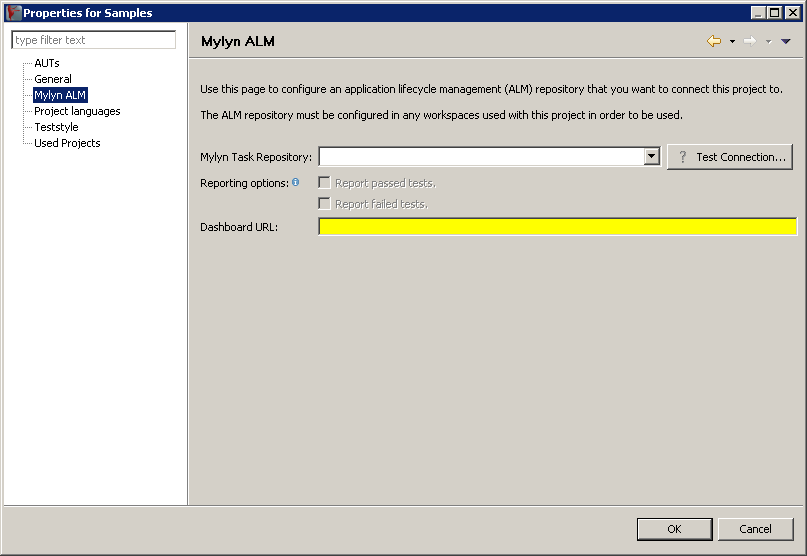
\includegraphics[width=12.5cm]{Tasks/ALM/PS/almproperties}
\caption{ALM Settings}
\label{TasksALMProjectProperties}
\end{center}
\end{figure}


\subsection{Adding task IDs to \gdjobs{}, \gdsuites{} and \gdcases{}}
\label{TasksALMAddTask}
You can add a task ID to \gdcases{}, \gdsuites{} and \gdjobs{} in your \gdproject{}. 

The task ID should be a valid ID in the repository that you have specified as the repository for this \gdproject{} \bxpref{TasksALMConfigureProject}. Adding the task ID to an item in your \gdproject{} means that this item is the relevant test for that task in your repository. When you activate the option, any test results for this item will be added as a comment to the task in the repository. The comment will include a link to the dashboard, in which the test result report can be viewed.

To add a task ID to a \gdcase{}, \gdsuite{} or \gdjob{}:
\begin{enumerate}
\item Open the item in the editor by double-clicking it.
\item In the \gdpropview{}, in the cell for \bxname{Task ID}, enter the task ID from the external repository. You can only enter task IDs at the place of specification -- you cannot overwrite them when you reuse the item.
\item Save the editor. 
\item When you have added a task ID to a node, you can open the task for this node from the browser by selecting:\\
\bxmenu{Open with}{Mylyn Task Editor}{}
\end{enumerate}

\bxtipp{You should ensure that you add task IDs to the right node-level to provide you with the relevant amount of information for the tasks in your repository. This will usually be at the level of Use Cases within a \gdsuite{}. }




\clearpage

\section{Object mapping}
The amount of keywords you have in a \app{} test and the amount of components your test deals with can grow very quickly. For this reason, it is important to think about structuring the \gdtestcasebrowser{} and the \gdomeditor{} to make finding \gdcases{} and component names easier. 


\subsection{Configuring task repositories in your workspace}
\label{TasksALMConfigureWorkspace}
Each repository you want to work with in your \ite{} must be configured in the workspace you are using. 

\begin{enumerate}
\item Select:\\ \bxmenu{Window}{Show View}{Other}\\ from the menu.
\item In the \bxname{Mylyn} section, select \bxname{Task Repositories} and click \bxcaption{OK}. The \bxname{Task Repositories} View will appear. The Bugzilla Repositories for \gd{} and \jb{} are pre-configured.
\item In the \bxname{Task Repositories} View, right click and select \bxname{Add Task Repository} from the context menu.
\item In the dialog that appears, you will see the pre-defined task repositories for the \ite{}. You can select one of these or choose to install a different connector. Depending on the connector you want to use, you may require additional software from Tasktop, or the connector may incur license fees.
\item Once you have selected your connector, click \bxcaption{Next}.
\item On the following page, you will need to configure the task repository. Please refer to the Mylyn documentation for information on repository configuration. 
\item Click \bxcaption{Finish} once the repository is configured.
\item To be able to see tasks in this repository, select: \\ \bxmenu{Window}{Show View}{Other}\\ from the menu. 
\item In the \bxname{Mylyn} section, select \bxname{Task List} and click \bxcaption{OK}. The \bxname{Task List} View will appear.
\end{enumerate}

You will now be able to see items in this repository, open them in the \ite{}, add queries for your workspace and work on tasks from this repository. 
You will also be able to select this repository in the \gdproject{} properties as the repository for your \gdproject{} \bxpref{TasksALMConfigureProject}. 


\subsection{Working on tasks in the \ite{}: contexts}
Once you have configured a task repository for your workspace \bxpref{TasksALMConfigureWorkspace}, you can work on tasks from that repository. 

\subsubsection{Opening and editing tasks in the \ite{}}
\begin{itemize}
\item To be able to see tasks in a repository, select: \\ \bxmenu{Window}{Show View}{Other}\\ from the menu. 
\item In the \bxname{Mylyn} section, select \bxname{Task List} and click \bxcaption{OK}. The \bxname{Task List} View will appear.
\item Double-click on a task to open this task in the editor area.
\item Once a task is open, you can work on it as you would in an external system -- add comments, change status etc.
\end{itemize}

\subsubsection{Working on tasks in the \ite{}}
\label{TasksActivateTask}
Mylyn supports context- or task-based working. When you work on a task, you only see items relevant to that task, so that coming back to the task later involves less context-switching. 
\begin{itemize}
\item Mylyn supports context-based working. You can work on existing tasks in a configured repository, or you can create tasks to work on.
\item To work on a task, you must \bxname{activate} it. To activate a task, select the task in the \bxname{Task List} and select:\\ \bxmenu{Activate}{}{}\\
from the context-sensitive menu. 
\item When you activate a task for the first time, the browsers and editors will seem very empty. This is because nothing is yet a part of the context for this task.
\item You can navigate through the browsers by pressing \bxkey{Alt+Click} to expand each level, or you can press the \bxname{Focus on task} button in the browsers to show the whole tree (not focusing on the task), or just the items in the current context (focusing on the task). 
\item Items are automatically added to your context when you select them in a browser, when you open them in an editor, or when you perform other actions that cause them to be made relevant (e.g. \gdcase{} creation, showing a \gdcase{} specification etc.). Items that are used particularly frequently are marked as \bxname{landmarks} and shown in bold. 
\item You can manually alter which items are in your context using the context-sensitive menu for a specific item. You can manually make items landmarks, or remove them from the context. 
\item The context that is created for you will be re-created when you reactivate the task at a later point. 
\end{itemize}



\subsection{Creating tasks in external repositories from test result reports}
\gdhelpid{testResultViewContextId}{Test Results View}
 You can create a new task with pre-filled information directly from an open test result report in the \gdtestresultview{}. This is useful if a test has failed and you want to create e.g. an issue in your bug-tracking system for the failure. 
\begin{enumerate}
\item In an open test result report, select the node that best describes the test failure (e.g. a \gdcase{} or \gdstep{} that has failed, or the whole \gdsuite{}, then right-click and select:\\
\bxmenu{Create a Mylyn Task}{}{}\\
from the context-sensitive menu.
\item  In the dialog that appears, select a repository in which to create the task. A \bxname{local} repository is available by default, but you can also add connections to Bugzilla and Trac repositories by clicking \bxcaption{Add Task Repository} in the New Task Dialog. Connectors to other repositories can also be added. See the Mylyn documentation for more details on adding repositories.
\item Click \bxcaption{Finish} once you have selected your repository. 
\item The editor for a new task will appear. It is pre-filled with information relevant to the node that you selected. Edit the task to make it descriptive enough for a bug report and save the editor. 
\item Once you have created a task, you can activate it to start saving your context for this task. See the later section \bxpref{TasksActivateTask} for details.
\end{enumerate}


\subsection{Configuring a task repository for your \gdproject{}}
\label{TasksALMConfigureProject}
Once you have configured one or more repositories for your workspace \bxpref{}, you can select one of these to be the test-relevant repository for your \gdproject{}. 

This will let you:
\begin{itemize}
\item Add a task ID from this repository to \gdcases{}, \gdsuites{}, and \gdjobs{} in the \gdproject{} to signify that this item is the test for this task \bxpref{TasksALMAddTask}.
\item Automatically report test results to the task defined when a test runs.
\item View the test results for the relevant item in the dashboard as a link from the task repository.
\end{itemize}

To configure a task repository for your \gdproject{}:

\begin{enumerate}
\item In the \gdproject{} Properties, select \bxname{Mylyn ALM} from the tree on the left \bxfigref{TasksALMProjectProperties}.
\item In the page that appears, you can select a repository from the combo-box.
\item You can then choose whether to only report failed tests, only report successful tests, or both.
\item Enter the URL of the \dash{} that is configured to use the correct \gddb{} for your test results. This is the \dash{} that will be opened when you click on a test result link from the task repository.
\end{enumerate}

\begin{figure}[h]
\begin{center}
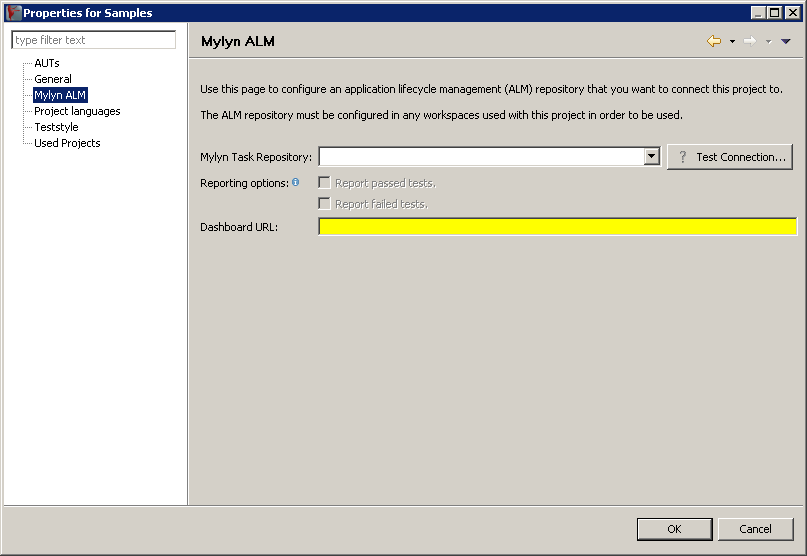
\includegraphics[width=12.5cm]{Tasks/ALM/PS/almproperties}
\caption{ALM Settings}
\label{TasksALMProjectProperties}
\end{center}
\end{figure}


\subsection{Adding task IDs to \gdjobs{}, \gdsuites{} and \gdcases{}}
\label{TasksALMAddTask}
You can add a task ID to \gdcases{}, \gdsuites{} and \gdjobs{} in your \gdproject{}. 

The task ID should be a valid ID in the repository that you have specified as the repository for this \gdproject{} \bxpref{TasksALMConfigureProject}. Adding the task ID to an item in your \gdproject{} means that this item is the relevant test for that task in your repository. When you activate the option, any test results for this item will be added as a comment to the task in the repository. The comment will include a link to the dashboard, in which the test result report can be viewed.

To add a task ID to a \gdcase{}, \gdsuite{} or \gdjob{}:
\begin{enumerate}
\item Open the item in the editor by double-clicking it.
\item In the \gdpropview{}, in the cell for \bxname{Task ID}, enter the task ID from the external repository. You can only enter task IDs at the place of specification -- you cannot overwrite them when you reuse the item.
\item Save the editor. 
\item When you have added a task ID to a node, you can open the task for this node from the browser by selecting:\\
\bxmenu{Open with}{Mylyn Task Editor}{}
\end{enumerate}

\bxtipp{You should ensure that you add task IDs to the right node-level to provide you with the relevant amount of information for the tasks in your repository. This will usually be at the level of Use Cases within a \gdsuite{}. }




\clearpage

\section{Test execution}
\label{TestExec}
The amount of keywords you have in a \app{} test and the amount of components your test deals with can grow very quickly. For this reason, it is important to think about structuring the \gdtestcasebrowser{} and the \gdomeditor{} to make finding \gdcases{} and component names easier. 


\subsection{Configuring task repositories in your workspace}
\label{TasksALMConfigureWorkspace}
Each repository you want to work with in your \ite{} must be configured in the workspace you are using. 

\begin{enumerate}
\item Select:\\ \bxmenu{Window}{Show View}{Other}\\ from the menu.
\item In the \bxname{Mylyn} section, select \bxname{Task Repositories} and click \bxcaption{OK}. The \bxname{Task Repositories} View will appear. The Bugzilla Repositories for \gd{} and \jb{} are pre-configured.
\item In the \bxname{Task Repositories} View, right click and select \bxname{Add Task Repository} from the context menu.
\item In the dialog that appears, you will see the pre-defined task repositories for the \ite{}. You can select one of these or choose to install a different connector. Depending on the connector you want to use, you may require additional software from Tasktop, or the connector may incur license fees.
\item Once you have selected your connector, click \bxcaption{Next}.
\item On the following page, you will need to configure the task repository. Please refer to the Mylyn documentation for information on repository configuration. 
\item Click \bxcaption{Finish} once the repository is configured.
\item To be able to see tasks in this repository, select: \\ \bxmenu{Window}{Show View}{Other}\\ from the menu. 
\item In the \bxname{Mylyn} section, select \bxname{Task List} and click \bxcaption{OK}. The \bxname{Task List} View will appear.
\end{enumerate}

You will now be able to see items in this repository, open them in the \ite{}, add queries for your workspace and work on tasks from this repository. 
You will also be able to select this repository in the \gdproject{} properties as the repository for your \gdproject{} \bxpref{TasksALMConfigureProject}. 


\subsection{Working on tasks in the \ite{}: contexts}
Once you have configured a task repository for your workspace \bxpref{TasksALMConfigureWorkspace}, you can work on tasks from that repository. 

\subsubsection{Opening and editing tasks in the \ite{}}
\begin{itemize}
\item To be able to see tasks in a repository, select: \\ \bxmenu{Window}{Show View}{Other}\\ from the menu. 
\item In the \bxname{Mylyn} section, select \bxname{Task List} and click \bxcaption{OK}. The \bxname{Task List} View will appear.
\item Double-click on a task to open this task in the editor area.
\item Once a task is open, you can work on it as you would in an external system -- add comments, change status etc.
\end{itemize}

\subsubsection{Working on tasks in the \ite{}}
\label{TasksActivateTask}
Mylyn supports context- or task-based working. When you work on a task, you only see items relevant to that task, so that coming back to the task later involves less context-switching. 
\begin{itemize}
\item Mylyn supports context-based working. You can work on existing tasks in a configured repository, or you can create tasks to work on.
\item To work on a task, you must \bxname{activate} it. To activate a task, select the task in the \bxname{Task List} and select:\\ \bxmenu{Activate}{}{}\\
from the context-sensitive menu. 
\item When you activate a task for the first time, the browsers and editors will seem very empty. This is because nothing is yet a part of the context for this task.
\item You can navigate through the browsers by pressing \bxkey{Alt+Click} to expand each level, or you can press the \bxname{Focus on task} button in the browsers to show the whole tree (not focusing on the task), or just the items in the current context (focusing on the task). 
\item Items are automatically added to your context when you select them in a browser, when you open them in an editor, or when you perform other actions that cause them to be made relevant (e.g. \gdcase{} creation, showing a \gdcase{} specification etc.). Items that are used particularly frequently are marked as \bxname{landmarks} and shown in bold. 
\item You can manually alter which items are in your context using the context-sensitive menu for a specific item. You can manually make items landmarks, or remove them from the context. 
\item The context that is created for you will be re-created when you reactivate the task at a later point. 
\end{itemize}



\subsection{Creating tasks in external repositories from test result reports}
\gdhelpid{testResultViewContextId}{Test Results View}
 You can create a new task with pre-filled information directly from an open test result report in the \gdtestresultview{}. This is useful if a test has failed and you want to create e.g. an issue in your bug-tracking system for the failure. 
\begin{enumerate}
\item In an open test result report, select the node that best describes the test failure (e.g. a \gdcase{} or \gdstep{} that has failed, or the whole \gdsuite{}, then right-click and select:\\
\bxmenu{Create a Mylyn Task}{}{}\\
from the context-sensitive menu.
\item  In the dialog that appears, select a repository in which to create the task. A \bxname{local} repository is available by default, but you can also add connections to Bugzilla and Trac repositories by clicking \bxcaption{Add Task Repository} in the New Task Dialog. Connectors to other repositories can also be added. See the Mylyn documentation for more details on adding repositories.
\item Click \bxcaption{Finish} once you have selected your repository. 
\item The editor for a new task will appear. It is pre-filled with information relevant to the node that you selected. Edit the task to make it descriptive enough for a bug report and save the editor. 
\item Once you have created a task, you can activate it to start saving your context for this task. See the later section \bxpref{TasksActivateTask} for details.
\end{enumerate}


\subsection{Configuring a task repository for your \gdproject{}}
\label{TasksALMConfigureProject}
Once you have configured one or more repositories for your workspace \bxpref{}, you can select one of these to be the test-relevant repository for your \gdproject{}. 

This will let you:
\begin{itemize}
\item Add a task ID from this repository to \gdcases{}, \gdsuites{}, and \gdjobs{} in the \gdproject{} to signify that this item is the test for this task \bxpref{TasksALMAddTask}.
\item Automatically report test results to the task defined when a test runs.
\item View the test results for the relevant item in the dashboard as a link from the task repository.
\end{itemize}

To configure a task repository for your \gdproject{}:

\begin{enumerate}
\item In the \gdproject{} Properties, select \bxname{Mylyn ALM} from the tree on the left \bxfigref{TasksALMProjectProperties}.
\item In the page that appears, you can select a repository from the combo-box.
\item You can then choose whether to only report failed tests, only report successful tests, or both.
\item Enter the URL of the \dash{} that is configured to use the correct \gddb{} for your test results. This is the \dash{} that will be opened when you click on a test result link from the task repository.
\end{enumerate}

\begin{figure}[h]
\begin{center}
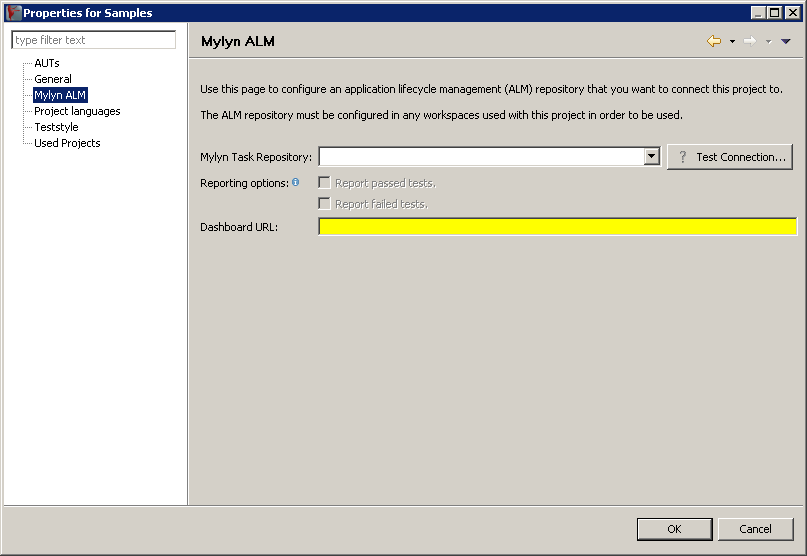
\includegraphics[width=12.5cm]{Tasks/ALM/PS/almproperties}
\caption{ALM Settings}
\label{TasksALMProjectProperties}
\end{center}
\end{figure}


\subsection{Adding task IDs to \gdjobs{}, \gdsuites{} and \gdcases{}}
\label{TasksALMAddTask}
You can add a task ID to \gdcases{}, \gdsuites{} and \gdjobs{} in your \gdproject{}. 

The task ID should be a valid ID in the repository that you have specified as the repository for this \gdproject{} \bxpref{TasksALMConfigureProject}. Adding the task ID to an item in your \gdproject{} means that this item is the relevant test for that task in your repository. When you activate the option, any test results for this item will be added as a comment to the task in the repository. The comment will include a link to the dashboard, in which the test result report can be viewed.

To add a task ID to a \gdcase{}, \gdsuite{} or \gdjob{}:
\begin{enumerate}
\item Open the item in the editor by double-clicking it.
\item In the \gdpropview{}, in the cell for \bxname{Task ID}, enter the task ID from the external repository. You can only enter task IDs at the place of specification -- you cannot overwrite them when you reuse the item.
\item Save the editor. 
\item When you have added a task ID to a node, you can open the task for this node from the browser by selecting:\\
\bxmenu{Open with}{Mylyn Task Editor}{}
\end{enumerate}

\bxtipp{You should ensure that you add task IDs to the right node-level to provide you with the relevant amount of information for the tasks in your repository. This will usually be at the level of Use Cases within a \gdsuite{}. }




\clearpage

\section{Working with test results}
The amount of keywords you have in a \app{} test and the amount of components your test deals with can grow very quickly. For this reason, it is important to think about structuring the \gdtestcasebrowser{} and the \gdomeditor{} to make finding \gdcases{} and component names easier. 


\subsection{Configuring task repositories in your workspace}
\label{TasksALMConfigureWorkspace}
Each repository you want to work with in your \ite{} must be configured in the workspace you are using. 

\begin{enumerate}
\item Select:\\ \bxmenu{Window}{Show View}{Other}\\ from the menu.
\item In the \bxname{Mylyn} section, select \bxname{Task Repositories} and click \bxcaption{OK}. The \bxname{Task Repositories} View will appear. The Bugzilla Repositories for \gd{} and \jb{} are pre-configured.
\item In the \bxname{Task Repositories} View, right click and select \bxname{Add Task Repository} from the context menu.
\item In the dialog that appears, you will see the pre-defined task repositories for the \ite{}. You can select one of these or choose to install a different connector. Depending on the connector you want to use, you may require additional software from Tasktop, or the connector may incur license fees.
\item Once you have selected your connector, click \bxcaption{Next}.
\item On the following page, you will need to configure the task repository. Please refer to the Mylyn documentation for information on repository configuration. 
\item Click \bxcaption{Finish} once the repository is configured.
\item To be able to see tasks in this repository, select: \\ \bxmenu{Window}{Show View}{Other}\\ from the menu. 
\item In the \bxname{Mylyn} section, select \bxname{Task List} and click \bxcaption{OK}. The \bxname{Task List} View will appear.
\end{enumerate}

You will now be able to see items in this repository, open them in the \ite{}, add queries for your workspace and work on tasks from this repository. 
You will also be able to select this repository in the \gdproject{} properties as the repository for your \gdproject{} \bxpref{TasksALMConfigureProject}. 


\subsection{Working on tasks in the \ite{}: contexts}
Once you have configured a task repository for your workspace \bxpref{TasksALMConfigureWorkspace}, you can work on tasks from that repository. 

\subsubsection{Opening and editing tasks in the \ite{}}
\begin{itemize}
\item To be able to see tasks in a repository, select: \\ \bxmenu{Window}{Show View}{Other}\\ from the menu. 
\item In the \bxname{Mylyn} section, select \bxname{Task List} and click \bxcaption{OK}. The \bxname{Task List} View will appear.
\item Double-click on a task to open this task in the editor area.
\item Once a task is open, you can work on it as you would in an external system -- add comments, change status etc.
\end{itemize}

\subsubsection{Working on tasks in the \ite{}}
\label{TasksActivateTask}
Mylyn supports context- or task-based working. When you work on a task, you only see items relevant to that task, so that coming back to the task later involves less context-switching. 
\begin{itemize}
\item Mylyn supports context-based working. You can work on existing tasks in a configured repository, or you can create tasks to work on.
\item To work on a task, you must \bxname{activate} it. To activate a task, select the task in the \bxname{Task List} and select:\\ \bxmenu{Activate}{}{}\\
from the context-sensitive menu. 
\item When you activate a task for the first time, the browsers and editors will seem very empty. This is because nothing is yet a part of the context for this task.
\item You can navigate through the browsers by pressing \bxkey{Alt+Click} to expand each level, or you can press the \bxname{Focus on task} button in the browsers to show the whole tree (not focusing on the task), or just the items in the current context (focusing on the task). 
\item Items are automatically added to your context when you select them in a browser, when you open them in an editor, or when you perform other actions that cause them to be made relevant (e.g. \gdcase{} creation, showing a \gdcase{} specification etc.). Items that are used particularly frequently are marked as \bxname{landmarks} and shown in bold. 
\item You can manually alter which items are in your context using the context-sensitive menu for a specific item. You can manually make items landmarks, or remove them from the context. 
\item The context that is created for you will be re-created when you reactivate the task at a later point. 
\end{itemize}



\subsection{Creating tasks in external repositories from test result reports}
\gdhelpid{testResultViewContextId}{Test Results View}
 You can create a new task with pre-filled information directly from an open test result report in the \gdtestresultview{}. This is useful if a test has failed and you want to create e.g. an issue in your bug-tracking system for the failure. 
\begin{enumerate}
\item In an open test result report, select the node that best describes the test failure (e.g. a \gdcase{} or \gdstep{} that has failed, or the whole \gdsuite{}, then right-click and select:\\
\bxmenu{Create a Mylyn Task}{}{}\\
from the context-sensitive menu.
\item  In the dialog that appears, select a repository in which to create the task. A \bxname{local} repository is available by default, but you can also add connections to Bugzilla and Trac repositories by clicking \bxcaption{Add Task Repository} in the New Task Dialog. Connectors to other repositories can also be added. See the Mylyn documentation for more details on adding repositories.
\item Click \bxcaption{Finish} once you have selected your repository. 
\item The editor for a new task will appear. It is pre-filled with information relevant to the node that you selected. Edit the task to make it descriptive enough for a bug report and save the editor. 
\item Once you have created a task, you can activate it to start saving your context for this task. See the later section \bxpref{TasksActivateTask} for details.
\end{enumerate}


\subsection{Configuring a task repository for your \gdproject{}}
\label{TasksALMConfigureProject}
Once you have configured one or more repositories for your workspace \bxpref{}, you can select one of these to be the test-relevant repository for your \gdproject{}. 

This will let you:
\begin{itemize}
\item Add a task ID from this repository to \gdcases{}, \gdsuites{}, and \gdjobs{} in the \gdproject{} to signify that this item is the test for this task \bxpref{TasksALMAddTask}.
\item Automatically report test results to the task defined when a test runs.
\item View the test results for the relevant item in the dashboard as a link from the task repository.
\end{itemize}

To configure a task repository for your \gdproject{}:

\begin{enumerate}
\item In the \gdproject{} Properties, select \bxname{Mylyn ALM} from the tree on the left \bxfigref{TasksALMProjectProperties}.
\item In the page that appears, you can select a repository from the combo-box.
\item You can then choose whether to only report failed tests, only report successful tests, or both.
\item Enter the URL of the \dash{} that is configured to use the correct \gddb{} for your test results. This is the \dash{} that will be opened when you click on a test result link from the task repository.
\end{enumerate}

\begin{figure}[h]
\begin{center}
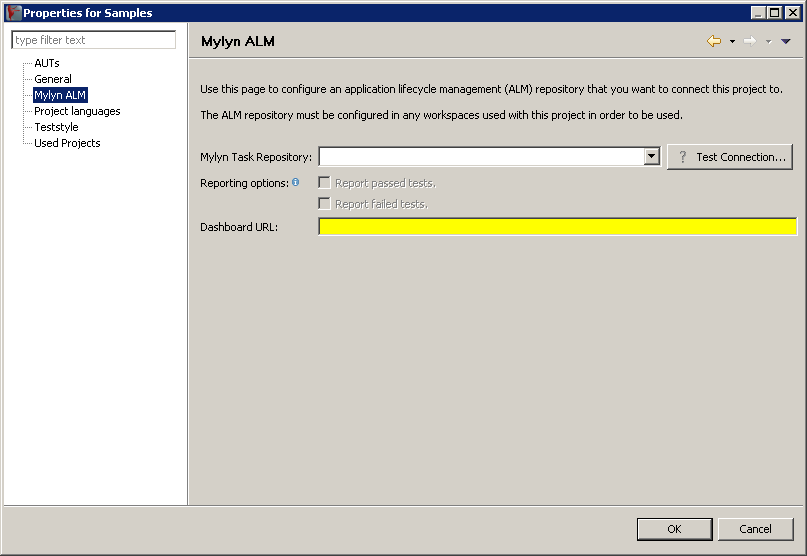
\includegraphics[width=12.5cm]{Tasks/ALM/PS/almproperties}
\caption{ALM Settings}
\label{TasksALMProjectProperties}
\end{center}
\end{figure}


\subsection{Adding task IDs to \gdjobs{}, \gdsuites{} and \gdcases{}}
\label{TasksALMAddTask}
You can add a task ID to \gdcases{}, \gdsuites{} and \gdjobs{} in your \gdproject{}. 

The task ID should be a valid ID in the repository that you have specified as the repository for this \gdproject{} \bxpref{TasksALMConfigureProject}. Adding the task ID to an item in your \gdproject{} means that this item is the relevant test for that task in your repository. When you activate the option, any test results for this item will be added as a comment to the task in the repository. The comment will include a link to the dashboard, in which the test result report can be viewed.

To add a task ID to a \gdcase{}, \gdsuite{} or \gdjob{}:
\begin{enumerate}
\item Open the item in the editor by double-clicking it.
\item In the \gdpropview{}, in the cell for \bxname{Task ID}, enter the task ID from the external repository. You can only enter task IDs at the place of specification -- you cannot overwrite them when you reuse the item.
\item Save the editor. 
\item When you have added a task ID to a node, you can open the task for this node from the browser by selecting:\\
\bxmenu{Open with}{Mylyn Task Editor}{}
\end{enumerate}

\bxtipp{You should ensure that you add task IDs to the right node-level to provide you with the relevant amount of information for the tasks in your repository. This will usually be at the level of Use Cases within a \gdsuite{}. }




\clearpage

\section{Dealing with errors in tests: \gdehandlers{}}
\gdhelpid{guidancerSpecTestCaseEditorContextId}{Test Case Editor}
\gdhelpid{eventHandlerAddContextId}{Event Handlers}
\gdhelpid{testExecViewContextId}{Test Suite Browser}
\label{customizedehandler}
The amount of keywords you have in a \app{} test and the amount of components your test deals with can grow very quickly. For this reason, it is important to think about structuring the \gdtestcasebrowser{} and the \gdomeditor{} to make finding \gdcases{} and component names easier. 


\subsection{Configuring task repositories in your workspace}
\label{TasksALMConfigureWorkspace}
Each repository you want to work with in your \ite{} must be configured in the workspace you are using. 

\begin{enumerate}
\item Select:\\ \bxmenu{Window}{Show View}{Other}\\ from the menu.
\item In the \bxname{Mylyn} section, select \bxname{Task Repositories} and click \bxcaption{OK}. The \bxname{Task Repositories} View will appear. The Bugzilla Repositories for \gd{} and \jb{} are pre-configured.
\item In the \bxname{Task Repositories} View, right click and select \bxname{Add Task Repository} from the context menu.
\item In the dialog that appears, you will see the pre-defined task repositories for the \ite{}. You can select one of these or choose to install a different connector. Depending on the connector you want to use, you may require additional software from Tasktop, or the connector may incur license fees.
\item Once you have selected your connector, click \bxcaption{Next}.
\item On the following page, you will need to configure the task repository. Please refer to the Mylyn documentation for information on repository configuration. 
\item Click \bxcaption{Finish} once the repository is configured.
\item To be able to see tasks in this repository, select: \\ \bxmenu{Window}{Show View}{Other}\\ from the menu. 
\item In the \bxname{Mylyn} section, select \bxname{Task List} and click \bxcaption{OK}. The \bxname{Task List} View will appear.
\end{enumerate}

You will now be able to see items in this repository, open them in the \ite{}, add queries for your workspace and work on tasks from this repository. 
You will also be able to select this repository in the \gdproject{} properties as the repository for your \gdproject{} \bxpref{TasksALMConfigureProject}. 


\subsection{Working on tasks in the \ite{}: contexts}
Once you have configured a task repository for your workspace \bxpref{TasksALMConfigureWorkspace}, you can work on tasks from that repository. 

\subsubsection{Opening and editing tasks in the \ite{}}
\begin{itemize}
\item To be able to see tasks in a repository, select: \\ \bxmenu{Window}{Show View}{Other}\\ from the menu. 
\item In the \bxname{Mylyn} section, select \bxname{Task List} and click \bxcaption{OK}. The \bxname{Task List} View will appear.
\item Double-click on a task to open this task in the editor area.
\item Once a task is open, you can work on it as you would in an external system -- add comments, change status etc.
\end{itemize}

\subsubsection{Working on tasks in the \ite{}}
\label{TasksActivateTask}
Mylyn supports context- or task-based working. When you work on a task, you only see items relevant to that task, so that coming back to the task later involves less context-switching. 
\begin{itemize}
\item Mylyn supports context-based working. You can work on existing tasks in a configured repository, or you can create tasks to work on.
\item To work on a task, you must \bxname{activate} it. To activate a task, select the task in the \bxname{Task List} and select:\\ \bxmenu{Activate}{}{}\\
from the context-sensitive menu. 
\item When you activate a task for the first time, the browsers and editors will seem very empty. This is because nothing is yet a part of the context for this task.
\item You can navigate through the browsers by pressing \bxkey{Alt+Click} to expand each level, or you can press the \bxname{Focus on task} button in the browsers to show the whole tree (not focusing on the task), or just the items in the current context (focusing on the task). 
\item Items are automatically added to your context when you select them in a browser, when you open them in an editor, or when you perform other actions that cause them to be made relevant (e.g. \gdcase{} creation, showing a \gdcase{} specification etc.). Items that are used particularly frequently are marked as \bxname{landmarks} and shown in bold. 
\item You can manually alter which items are in your context using the context-sensitive menu for a specific item. You can manually make items landmarks, or remove them from the context. 
\item The context that is created for you will be re-created when you reactivate the task at a later point. 
\end{itemize}



\subsection{Creating tasks in external repositories from test result reports}
\gdhelpid{testResultViewContextId}{Test Results View}
 You can create a new task with pre-filled information directly from an open test result report in the \gdtestresultview{}. This is useful if a test has failed and you want to create e.g. an issue in your bug-tracking system for the failure. 
\begin{enumerate}
\item In an open test result report, select the node that best describes the test failure (e.g. a \gdcase{} or \gdstep{} that has failed, or the whole \gdsuite{}, then right-click and select:\\
\bxmenu{Create a Mylyn Task}{}{}\\
from the context-sensitive menu.
\item  In the dialog that appears, select a repository in which to create the task. A \bxname{local} repository is available by default, but you can also add connections to Bugzilla and Trac repositories by clicking \bxcaption{Add Task Repository} in the New Task Dialog. Connectors to other repositories can also be added. See the Mylyn documentation for more details on adding repositories.
\item Click \bxcaption{Finish} once you have selected your repository. 
\item The editor for a new task will appear. It is pre-filled with information relevant to the node that you selected. Edit the task to make it descriptive enough for a bug report and save the editor. 
\item Once you have created a task, you can activate it to start saving your context for this task. See the later section \bxpref{TasksActivateTask} for details.
\end{enumerate}


\subsection{Configuring a task repository for your \gdproject{}}
\label{TasksALMConfigureProject}
Once you have configured one or more repositories for your workspace \bxpref{}, you can select one of these to be the test-relevant repository for your \gdproject{}. 

This will let you:
\begin{itemize}
\item Add a task ID from this repository to \gdcases{}, \gdsuites{}, and \gdjobs{} in the \gdproject{} to signify that this item is the test for this task \bxpref{TasksALMAddTask}.
\item Automatically report test results to the task defined when a test runs.
\item View the test results for the relevant item in the dashboard as a link from the task repository.
\end{itemize}

To configure a task repository for your \gdproject{}:

\begin{enumerate}
\item In the \gdproject{} Properties, select \bxname{Mylyn ALM} from the tree on the left \bxfigref{TasksALMProjectProperties}.
\item In the page that appears, you can select a repository from the combo-box.
\item You can then choose whether to only report failed tests, only report successful tests, or both.
\item Enter the URL of the \dash{} that is configured to use the correct \gddb{} for your test results. This is the \dash{} that will be opened when you click on a test result link from the task repository.
\end{enumerate}

\begin{figure}[h]
\begin{center}
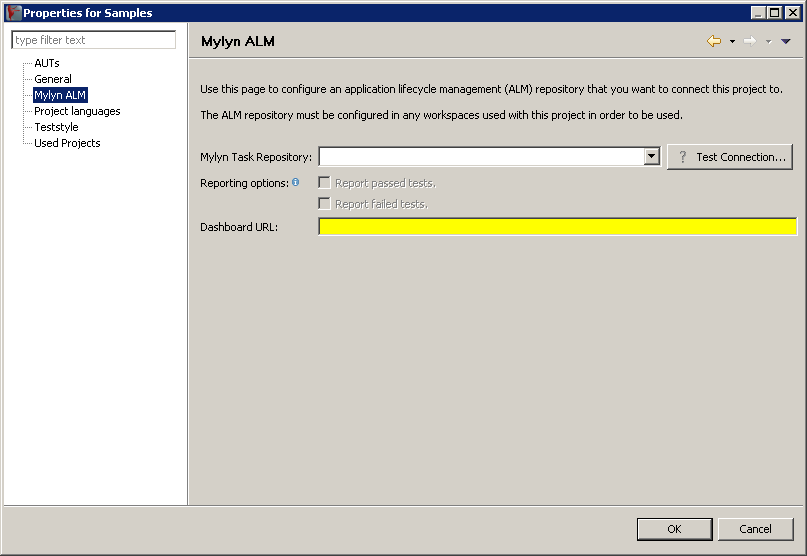
\includegraphics[width=12.5cm]{Tasks/ALM/PS/almproperties}
\caption{ALM Settings}
\label{TasksALMProjectProperties}
\end{center}
\end{figure}


\subsection{Adding task IDs to \gdjobs{}, \gdsuites{} and \gdcases{}}
\label{TasksALMAddTask}
You can add a task ID to \gdcases{}, \gdsuites{} and \gdjobs{} in your \gdproject{}. 

The task ID should be a valid ID in the repository that you have specified as the repository for this \gdproject{} \bxpref{TasksALMConfigureProject}. Adding the task ID to an item in your \gdproject{} means that this item is the relevant test for that task in your repository. When you activate the option, any test results for this item will be added as a comment to the task in the repository. The comment will include a link to the dashboard, in which the test result report can be viewed.

To add a task ID to a \gdcase{}, \gdsuite{} or \gdjob{}:
\begin{enumerate}
\item Open the item in the editor by double-clicking it.
\item In the \gdpropview{}, in the cell for \bxname{Task ID}, enter the task ID from the external repository. You can only enter task IDs at the place of specification -- you cannot overwrite them when you reuse the item.
\item Save the editor. 
\item When you have added a task ID to a node, you can open the task for this node from the browser by selecting:\\
\bxmenu{Open with}{Mylyn Task Editor}{}
\end{enumerate}

\bxtipp{You should ensure that you add task IDs to the right node-level to provide you with the relevant amount of information for the tasks in your repository. This will usually be at the level of Use Cases within a \gdsuite{}. }




\clearpage
\section{Preferences}
\label{ConfigurePrefs}
The amount of keywords you have in a \app{} test and the amount of components your test deals with can grow very quickly. For this reason, it is important to think about structuring the \gdtestcasebrowser{} and the \gdomeditor{} to make finding \gdcases{} and component names easier. 


\subsection{Configuring task repositories in your workspace}
\label{TasksALMConfigureWorkspace}
Each repository you want to work with in your \ite{} must be configured in the workspace you are using. 

\begin{enumerate}
\item Select:\\ \bxmenu{Window}{Show View}{Other}\\ from the menu.
\item In the \bxname{Mylyn} section, select \bxname{Task Repositories} and click \bxcaption{OK}. The \bxname{Task Repositories} View will appear. The Bugzilla Repositories for \gd{} and \jb{} are pre-configured.
\item In the \bxname{Task Repositories} View, right click and select \bxname{Add Task Repository} from the context menu.
\item In the dialog that appears, you will see the pre-defined task repositories for the \ite{}. You can select one of these or choose to install a different connector. Depending on the connector you want to use, you may require additional software from Tasktop, or the connector may incur license fees.
\item Once you have selected your connector, click \bxcaption{Next}.
\item On the following page, you will need to configure the task repository. Please refer to the Mylyn documentation for information on repository configuration. 
\item Click \bxcaption{Finish} once the repository is configured.
\item To be able to see tasks in this repository, select: \\ \bxmenu{Window}{Show View}{Other}\\ from the menu. 
\item In the \bxname{Mylyn} section, select \bxname{Task List} and click \bxcaption{OK}. The \bxname{Task List} View will appear.
\end{enumerate}

You will now be able to see items in this repository, open them in the \ite{}, add queries for your workspace and work on tasks from this repository. 
You will also be able to select this repository in the \gdproject{} properties as the repository for your \gdproject{} \bxpref{TasksALMConfigureProject}. 


\subsection{Working on tasks in the \ite{}: contexts}
Once you have configured a task repository for your workspace \bxpref{TasksALMConfigureWorkspace}, you can work on tasks from that repository. 

\subsubsection{Opening and editing tasks in the \ite{}}
\begin{itemize}
\item To be able to see tasks in a repository, select: \\ \bxmenu{Window}{Show View}{Other}\\ from the menu. 
\item In the \bxname{Mylyn} section, select \bxname{Task List} and click \bxcaption{OK}. The \bxname{Task List} View will appear.
\item Double-click on a task to open this task in the editor area.
\item Once a task is open, you can work on it as you would in an external system -- add comments, change status etc.
\end{itemize}

\subsubsection{Working on tasks in the \ite{}}
\label{TasksActivateTask}
Mylyn supports context- or task-based working. When you work on a task, you only see items relevant to that task, so that coming back to the task later involves less context-switching. 
\begin{itemize}
\item Mylyn supports context-based working. You can work on existing tasks in a configured repository, or you can create tasks to work on.
\item To work on a task, you must \bxname{activate} it. To activate a task, select the task in the \bxname{Task List} and select:\\ \bxmenu{Activate}{}{}\\
from the context-sensitive menu. 
\item When you activate a task for the first time, the browsers and editors will seem very empty. This is because nothing is yet a part of the context for this task.
\item You can navigate through the browsers by pressing \bxkey{Alt+Click} to expand each level, or you can press the \bxname{Focus on task} button in the browsers to show the whole tree (not focusing on the task), or just the items in the current context (focusing on the task). 
\item Items are automatically added to your context when you select them in a browser, when you open them in an editor, or when you perform other actions that cause them to be made relevant (e.g. \gdcase{} creation, showing a \gdcase{} specification etc.). Items that are used particularly frequently are marked as \bxname{landmarks} and shown in bold. 
\item You can manually alter which items are in your context using the context-sensitive menu for a specific item. You can manually make items landmarks, or remove them from the context. 
\item The context that is created for you will be re-created when you reactivate the task at a later point. 
\end{itemize}



\subsection{Creating tasks in external repositories from test result reports}
\gdhelpid{testResultViewContextId}{Test Results View}
 You can create a new task with pre-filled information directly from an open test result report in the \gdtestresultview{}. This is useful if a test has failed and you want to create e.g. an issue in your bug-tracking system for the failure. 
\begin{enumerate}
\item In an open test result report, select the node that best describes the test failure (e.g. a \gdcase{} or \gdstep{} that has failed, or the whole \gdsuite{}, then right-click and select:\\
\bxmenu{Create a Mylyn Task}{}{}\\
from the context-sensitive menu.
\item  In the dialog that appears, select a repository in which to create the task. A \bxname{local} repository is available by default, but you can also add connections to Bugzilla and Trac repositories by clicking \bxcaption{Add Task Repository} in the New Task Dialog. Connectors to other repositories can also be added. See the Mylyn documentation for more details on adding repositories.
\item Click \bxcaption{Finish} once you have selected your repository. 
\item The editor for a new task will appear. It is pre-filled with information relevant to the node that you selected. Edit the task to make it descriptive enough for a bug report and save the editor. 
\item Once you have created a task, you can activate it to start saving your context for this task. See the later section \bxpref{TasksActivateTask} for details.
\end{enumerate}


\subsection{Configuring a task repository for your \gdproject{}}
\label{TasksALMConfigureProject}
Once you have configured one or more repositories for your workspace \bxpref{}, you can select one of these to be the test-relevant repository for your \gdproject{}. 

This will let you:
\begin{itemize}
\item Add a task ID from this repository to \gdcases{}, \gdsuites{}, and \gdjobs{} in the \gdproject{} to signify that this item is the test for this task \bxpref{TasksALMAddTask}.
\item Automatically report test results to the task defined when a test runs.
\item View the test results for the relevant item in the dashboard as a link from the task repository.
\end{itemize}

To configure a task repository for your \gdproject{}:

\begin{enumerate}
\item In the \gdproject{} Properties, select \bxname{Mylyn ALM} from the tree on the left \bxfigref{TasksALMProjectProperties}.
\item In the page that appears, you can select a repository from the combo-box.
\item You can then choose whether to only report failed tests, only report successful tests, or both.
\item Enter the URL of the \dash{} that is configured to use the correct \gddb{} for your test results. This is the \dash{} that will be opened when you click on a test result link from the task repository.
\end{enumerate}

\begin{figure}[h]
\begin{center}
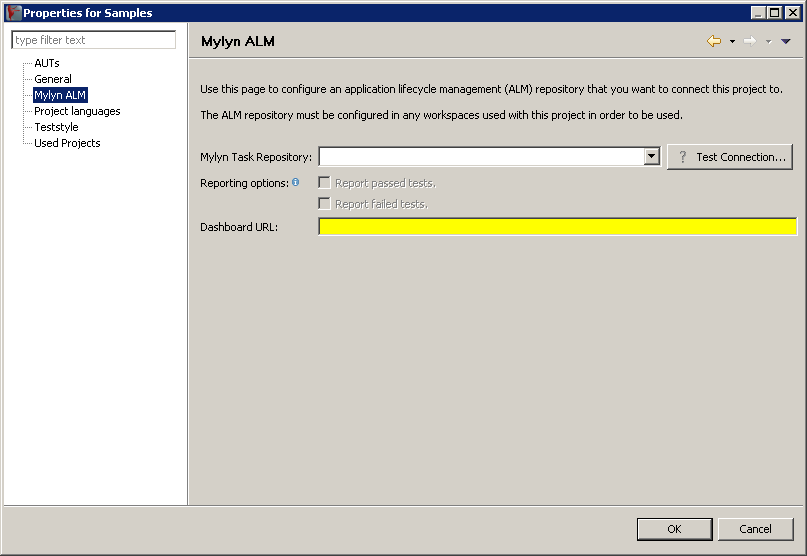
\includegraphics[width=12.5cm]{Tasks/ALM/PS/almproperties}
\caption{ALM Settings}
\label{TasksALMProjectProperties}
\end{center}
\end{figure}


\subsection{Adding task IDs to \gdjobs{}, \gdsuites{} and \gdcases{}}
\label{TasksALMAddTask}
You can add a task ID to \gdcases{}, \gdsuites{} and \gdjobs{} in your \gdproject{}. 

The task ID should be a valid ID in the repository that you have specified as the repository for this \gdproject{} \bxpref{TasksALMConfigureProject}. Adding the task ID to an item in your \gdproject{} means that this item is the relevant test for that task in your repository. When you activate the option, any test results for this item will be added as a comment to the task in the repository. The comment will include a link to the dashboard, in which the test result report can be viewed.

To add a task ID to a \gdcase{}, \gdsuite{} or \gdjob{}:
\begin{enumerate}
\item Open the item in the editor by double-clicking it.
\item In the \gdpropview{}, in the cell for \bxname{Task ID}, enter the task ID from the external repository. You can only enter task IDs at the place of specification -- you cannot overwrite them when you reuse the item.
\item Save the editor. 
\item When you have added a task ID to a node, you can open the task for this node from the browser by selecting:\\
\bxmenu{Open with}{Mylyn Task Editor}{}
\end{enumerate}

\bxtipp{You should ensure that you add task IDs to the right node-level to provide you with the relevant amount of information for the tasks in your repository. This will usually be at the level of Use Cases within a \gdsuite{}. }




\clearpage

\section{Observing \gdcases} 
\gdhelpid{guidancerSpecTestCaseEditorContextId}{Test Case Editor}
\gdhelpid{testSpecificationViewContextId}{Test Case Browser}
The amount of keywords you have in a \app{} test and the amount of components your test deals with can grow very quickly. For this reason, it is important to think about structuring the \gdtestcasebrowser{} and the \gdomeditor{} to make finding \gdcases{} and component names easier. 


\subsection{Configuring task repositories in your workspace}
\label{TasksALMConfigureWorkspace}
Each repository you want to work with in your \ite{} must be configured in the workspace you are using. 

\begin{enumerate}
\item Select:\\ \bxmenu{Window}{Show View}{Other}\\ from the menu.
\item In the \bxname{Mylyn} section, select \bxname{Task Repositories} and click \bxcaption{OK}. The \bxname{Task Repositories} View will appear. The Bugzilla Repositories for \gd{} and \jb{} are pre-configured.
\item In the \bxname{Task Repositories} View, right click and select \bxname{Add Task Repository} from the context menu.
\item In the dialog that appears, you will see the pre-defined task repositories for the \ite{}. You can select one of these or choose to install a different connector. Depending on the connector you want to use, you may require additional software from Tasktop, or the connector may incur license fees.
\item Once you have selected your connector, click \bxcaption{Next}.
\item On the following page, you will need to configure the task repository. Please refer to the Mylyn documentation for information on repository configuration. 
\item Click \bxcaption{Finish} once the repository is configured.
\item To be able to see tasks in this repository, select: \\ \bxmenu{Window}{Show View}{Other}\\ from the menu. 
\item In the \bxname{Mylyn} section, select \bxname{Task List} and click \bxcaption{OK}. The \bxname{Task List} View will appear.
\end{enumerate}

You will now be able to see items in this repository, open them in the \ite{}, add queries for your workspace and work on tasks from this repository. 
You will also be able to select this repository in the \gdproject{} properties as the repository for your \gdproject{} \bxpref{TasksALMConfigureProject}. 


\subsection{Working on tasks in the \ite{}: contexts}
Once you have configured a task repository for your workspace \bxpref{TasksALMConfigureWorkspace}, you can work on tasks from that repository. 

\subsubsection{Opening and editing tasks in the \ite{}}
\begin{itemize}
\item To be able to see tasks in a repository, select: \\ \bxmenu{Window}{Show View}{Other}\\ from the menu. 
\item In the \bxname{Mylyn} section, select \bxname{Task List} and click \bxcaption{OK}. The \bxname{Task List} View will appear.
\item Double-click on a task to open this task in the editor area.
\item Once a task is open, you can work on it as you would in an external system -- add comments, change status etc.
\end{itemize}

\subsubsection{Working on tasks in the \ite{}}
\label{TasksActivateTask}
Mylyn supports context- or task-based working. When you work on a task, you only see items relevant to that task, so that coming back to the task later involves less context-switching. 
\begin{itemize}
\item Mylyn supports context-based working. You can work on existing tasks in a configured repository, or you can create tasks to work on.
\item To work on a task, you must \bxname{activate} it. To activate a task, select the task in the \bxname{Task List} and select:\\ \bxmenu{Activate}{}{}\\
from the context-sensitive menu. 
\item When you activate a task for the first time, the browsers and editors will seem very empty. This is because nothing is yet a part of the context for this task.
\item You can navigate through the browsers by pressing \bxkey{Alt+Click} to expand each level, or you can press the \bxname{Focus on task} button in the browsers to show the whole tree (not focusing on the task), or just the items in the current context (focusing on the task). 
\item Items are automatically added to your context when you select them in a browser, when you open them in an editor, or when you perform other actions that cause them to be made relevant (e.g. \gdcase{} creation, showing a \gdcase{} specification etc.). Items that are used particularly frequently are marked as \bxname{landmarks} and shown in bold. 
\item You can manually alter which items are in your context using the context-sensitive menu for a specific item. You can manually make items landmarks, or remove them from the context. 
\item The context that is created for you will be re-created when you reactivate the task at a later point. 
\end{itemize}



\subsection{Creating tasks in external repositories from test result reports}
\gdhelpid{testResultViewContextId}{Test Results View}
 You can create a new task with pre-filled information directly from an open test result report in the \gdtestresultview{}. This is useful if a test has failed and you want to create e.g. an issue in your bug-tracking system for the failure. 
\begin{enumerate}
\item In an open test result report, select the node that best describes the test failure (e.g. a \gdcase{} or \gdstep{} that has failed, or the whole \gdsuite{}, then right-click and select:\\
\bxmenu{Create a Mylyn Task}{}{}\\
from the context-sensitive menu.
\item  In the dialog that appears, select a repository in which to create the task. A \bxname{local} repository is available by default, but you can also add connections to Bugzilla and Trac repositories by clicking \bxcaption{Add Task Repository} in the New Task Dialog. Connectors to other repositories can also be added. See the Mylyn documentation for more details on adding repositories.
\item Click \bxcaption{Finish} once you have selected your repository. 
\item The editor for a new task will appear. It is pre-filled with information relevant to the node that you selected. Edit the task to make it descriptive enough for a bug report and save the editor. 
\item Once you have created a task, you can activate it to start saving your context for this task. See the later section \bxpref{TasksActivateTask} for details.
\end{enumerate}


\subsection{Configuring a task repository for your \gdproject{}}
\label{TasksALMConfigureProject}
Once you have configured one or more repositories for your workspace \bxpref{}, you can select one of these to be the test-relevant repository for your \gdproject{}. 

This will let you:
\begin{itemize}
\item Add a task ID from this repository to \gdcases{}, \gdsuites{}, and \gdjobs{} in the \gdproject{} to signify that this item is the test for this task \bxpref{TasksALMAddTask}.
\item Automatically report test results to the task defined when a test runs.
\item View the test results for the relevant item in the dashboard as a link from the task repository.
\end{itemize}

To configure a task repository for your \gdproject{}:

\begin{enumerate}
\item In the \gdproject{} Properties, select \bxname{Mylyn ALM} from the tree on the left \bxfigref{TasksALMProjectProperties}.
\item In the page that appears, you can select a repository from the combo-box.
\item You can then choose whether to only report failed tests, only report successful tests, or both.
\item Enter the URL of the \dash{} that is configured to use the correct \gddb{} for your test results. This is the \dash{} that will be opened when you click on a test result link from the task repository.
\end{enumerate}

\begin{figure}[h]
\begin{center}
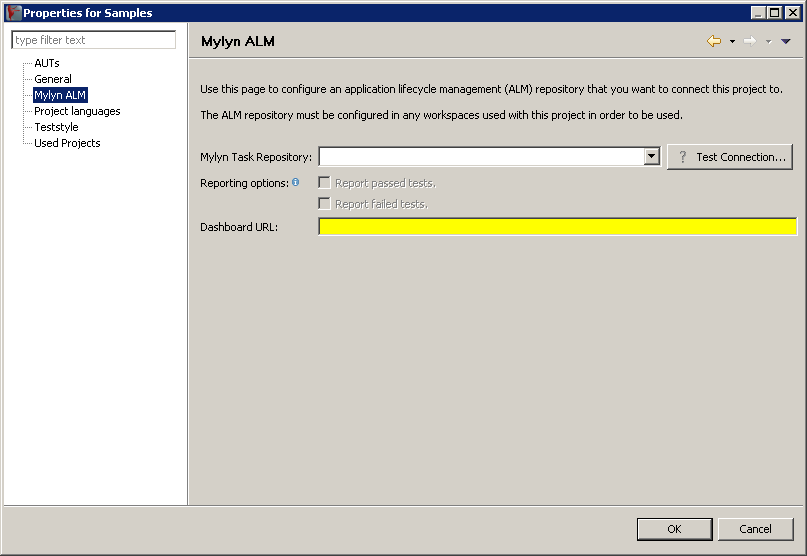
\includegraphics[width=12.5cm]{Tasks/ALM/PS/almproperties}
\caption{ALM Settings}
\label{TasksALMProjectProperties}
\end{center}
\end{figure}


\subsection{Adding task IDs to \gdjobs{}, \gdsuites{} and \gdcases{}}
\label{TasksALMAddTask}
You can add a task ID to \gdcases{}, \gdsuites{} and \gdjobs{} in your \gdproject{}. 

The task ID should be a valid ID in the repository that you have specified as the repository for this \gdproject{} \bxpref{TasksALMConfigureProject}. Adding the task ID to an item in your \gdproject{} means that this item is the relevant test for that task in your repository. When you activate the option, any test results for this item will be added as a comment to the task in the repository. The comment will include a link to the dashboard, in which the test result report can be viewed.

To add a task ID to a \gdcase{}, \gdsuite{} or \gdjob{}:
\begin{enumerate}
\item Open the item in the editor by double-clicking it.
\item In the \gdpropview{}, in the cell for \bxname{Task ID}, enter the task ID from the external repository. You can only enter task IDs at the place of specification -- you cannot overwrite them when you reuse the item.
\item Save the editor. 
\item When you have added a task ID to a node, you can open the task for this node from the browser by selecting:\\
\bxmenu{Open with}{Mylyn Task Editor}{}
\end{enumerate}

\bxtipp{You should ensure that you add task IDs to the right node-level to provide you with the relevant amount of information for the tasks in your repository. This will usually be at the level of Use Cases within a \gdsuite{}. }





\clearpage 

\section{Working with the \gdprobview}
The amount of keywords you have in a \app{} test and the amount of components your test deals with can grow very quickly. For this reason, it is important to think about structuring the \gdtestcasebrowser{} and the \gdomeditor{} to make finding \gdcases{} and component names easier. 


\subsection{Configuring task repositories in your workspace}
\label{TasksALMConfigureWorkspace}
Each repository you want to work with in your \ite{} must be configured in the workspace you are using. 

\begin{enumerate}
\item Select:\\ \bxmenu{Window}{Show View}{Other}\\ from the menu.
\item In the \bxname{Mylyn} section, select \bxname{Task Repositories} and click \bxcaption{OK}. The \bxname{Task Repositories} View will appear. The Bugzilla Repositories for \gd{} and \jb{} are pre-configured.
\item In the \bxname{Task Repositories} View, right click and select \bxname{Add Task Repository} from the context menu.
\item In the dialog that appears, you will see the pre-defined task repositories for the \ite{}. You can select one of these or choose to install a different connector. Depending on the connector you want to use, you may require additional software from Tasktop, or the connector may incur license fees.
\item Once you have selected your connector, click \bxcaption{Next}.
\item On the following page, you will need to configure the task repository. Please refer to the Mylyn documentation for information on repository configuration. 
\item Click \bxcaption{Finish} once the repository is configured.
\item To be able to see tasks in this repository, select: \\ \bxmenu{Window}{Show View}{Other}\\ from the menu. 
\item In the \bxname{Mylyn} section, select \bxname{Task List} and click \bxcaption{OK}. The \bxname{Task List} View will appear.
\end{enumerate}

You will now be able to see items in this repository, open them in the \ite{}, add queries for your workspace and work on tasks from this repository. 
You will also be able to select this repository in the \gdproject{} properties as the repository for your \gdproject{} \bxpref{TasksALMConfigureProject}. 


\subsection{Working on tasks in the \ite{}: contexts}
Once you have configured a task repository for your workspace \bxpref{TasksALMConfigureWorkspace}, you can work on tasks from that repository. 

\subsubsection{Opening and editing tasks in the \ite{}}
\begin{itemize}
\item To be able to see tasks in a repository, select: \\ \bxmenu{Window}{Show View}{Other}\\ from the menu. 
\item In the \bxname{Mylyn} section, select \bxname{Task List} and click \bxcaption{OK}. The \bxname{Task List} View will appear.
\item Double-click on a task to open this task in the editor area.
\item Once a task is open, you can work on it as you would in an external system -- add comments, change status etc.
\end{itemize}

\subsubsection{Working on tasks in the \ite{}}
\label{TasksActivateTask}
Mylyn supports context- or task-based working. When you work on a task, you only see items relevant to that task, so that coming back to the task later involves less context-switching. 
\begin{itemize}
\item Mylyn supports context-based working. You can work on existing tasks in a configured repository, or you can create tasks to work on.
\item To work on a task, you must \bxname{activate} it. To activate a task, select the task in the \bxname{Task List} and select:\\ \bxmenu{Activate}{}{}\\
from the context-sensitive menu. 
\item When you activate a task for the first time, the browsers and editors will seem very empty. This is because nothing is yet a part of the context for this task.
\item You can navigate through the browsers by pressing \bxkey{Alt+Click} to expand each level, or you can press the \bxname{Focus on task} button in the browsers to show the whole tree (not focusing on the task), or just the items in the current context (focusing on the task). 
\item Items are automatically added to your context when you select them in a browser, when you open them in an editor, or when you perform other actions that cause them to be made relevant (e.g. \gdcase{} creation, showing a \gdcase{} specification etc.). Items that are used particularly frequently are marked as \bxname{landmarks} and shown in bold. 
\item You can manually alter which items are in your context using the context-sensitive menu for a specific item. You can manually make items landmarks, or remove them from the context. 
\item The context that is created for you will be re-created when you reactivate the task at a later point. 
\end{itemize}



\subsection{Creating tasks in external repositories from test result reports}
\gdhelpid{testResultViewContextId}{Test Results View}
 You can create a new task with pre-filled information directly from an open test result report in the \gdtestresultview{}. This is useful if a test has failed and you want to create e.g. an issue in your bug-tracking system for the failure. 
\begin{enumerate}
\item In an open test result report, select the node that best describes the test failure (e.g. a \gdcase{} or \gdstep{} that has failed, or the whole \gdsuite{}, then right-click and select:\\
\bxmenu{Create a Mylyn Task}{}{}\\
from the context-sensitive menu.
\item  In the dialog that appears, select a repository in which to create the task. A \bxname{local} repository is available by default, but you can also add connections to Bugzilla and Trac repositories by clicking \bxcaption{Add Task Repository} in the New Task Dialog. Connectors to other repositories can also be added. See the Mylyn documentation for more details on adding repositories.
\item Click \bxcaption{Finish} once you have selected your repository. 
\item The editor for a new task will appear. It is pre-filled with information relevant to the node that you selected. Edit the task to make it descriptive enough for a bug report and save the editor. 
\item Once you have created a task, you can activate it to start saving your context for this task. See the later section \bxpref{TasksActivateTask} for details.
\end{enumerate}


\subsection{Configuring a task repository for your \gdproject{}}
\label{TasksALMConfigureProject}
Once you have configured one or more repositories for your workspace \bxpref{}, you can select one of these to be the test-relevant repository for your \gdproject{}. 

This will let you:
\begin{itemize}
\item Add a task ID from this repository to \gdcases{}, \gdsuites{}, and \gdjobs{} in the \gdproject{} to signify that this item is the test for this task \bxpref{TasksALMAddTask}.
\item Automatically report test results to the task defined when a test runs.
\item View the test results for the relevant item in the dashboard as a link from the task repository.
\end{itemize}

To configure a task repository for your \gdproject{}:

\begin{enumerate}
\item In the \gdproject{} Properties, select \bxname{Mylyn ALM} from the tree on the left \bxfigref{TasksALMProjectProperties}.
\item In the page that appears, you can select a repository from the combo-box.
\item You can then choose whether to only report failed tests, only report successful tests, or both.
\item Enter the URL of the \dash{} that is configured to use the correct \gddb{} for your test results. This is the \dash{} that will be opened when you click on a test result link from the task repository.
\end{enumerate}

\begin{figure}[h]
\begin{center}
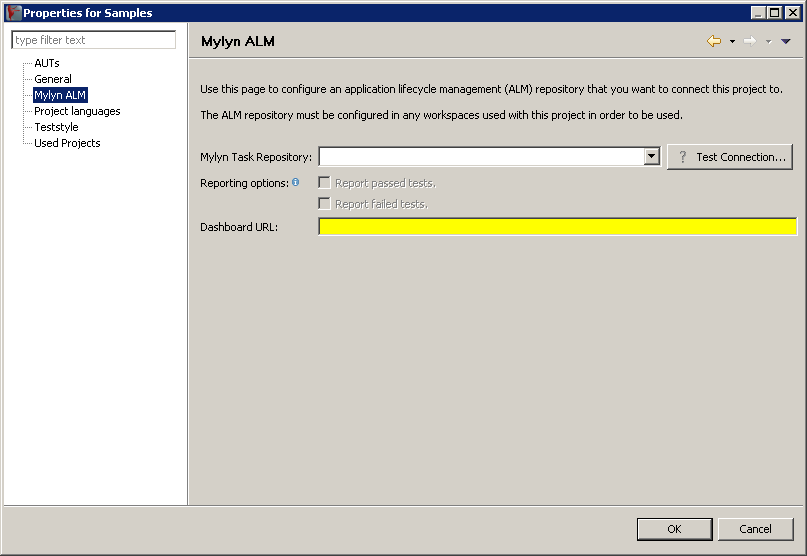
\includegraphics[width=12.5cm]{Tasks/ALM/PS/almproperties}
\caption{ALM Settings}
\label{TasksALMProjectProperties}
\end{center}
\end{figure}


\subsection{Adding task IDs to \gdjobs{}, \gdsuites{} and \gdcases{}}
\label{TasksALMAddTask}
You can add a task ID to \gdcases{}, \gdsuites{} and \gdjobs{} in your \gdproject{}. 

The task ID should be a valid ID in the repository that you have specified as the repository for this \gdproject{} \bxpref{TasksALMConfigureProject}. Adding the task ID to an item in your \gdproject{} means that this item is the relevant test for that task in your repository. When you activate the option, any test results for this item will be added as a comment to the task in the repository. The comment will include a link to the dashboard, in which the test result report can be viewed.

To add a task ID to a \gdcase{}, \gdsuite{} or \gdjob{}:
\begin{enumerate}
\item Open the item in the editor by double-clicking it.
\item In the \gdpropview{}, in the cell for \bxname{Task ID}, enter the task ID from the external repository. You can only enter task IDs at the place of specification -- you cannot overwrite them when you reuse the item.
\item Save the editor. 
\item When you have added a task ID to a node, you can open the task for this node from the browser by selecting:\\
\bxmenu{Open with}{Mylyn Task Editor}{}
\end{enumerate}

\bxtipp{You should ensure that you add task IDs to the right node-level to provide you with the relevant amount of information for the tasks in your repository. This will usually be at the level of Use Cases within a \gdsuite{}. }




\clearpage

\section{Adapting the user interface}
\gdhelpid{problemViewContextId}{Problem View}
The amount of keywords you have in a \app{} test and the amount of components your test deals with can grow very quickly. For this reason, it is important to think about structuring the \gdtestcasebrowser{} and the \gdomeditor{} to make finding \gdcases{} and component names easier. 


\subsection{Configuring task repositories in your workspace}
\label{TasksALMConfigureWorkspace}
Each repository you want to work with in your \ite{} must be configured in the workspace you are using. 

\begin{enumerate}
\item Select:\\ \bxmenu{Window}{Show View}{Other}\\ from the menu.
\item In the \bxname{Mylyn} section, select \bxname{Task Repositories} and click \bxcaption{OK}. The \bxname{Task Repositories} View will appear. The Bugzilla Repositories for \gd{} and \jb{} are pre-configured.
\item In the \bxname{Task Repositories} View, right click and select \bxname{Add Task Repository} from the context menu.
\item In the dialog that appears, you will see the pre-defined task repositories for the \ite{}. You can select one of these or choose to install a different connector. Depending on the connector you want to use, you may require additional software from Tasktop, or the connector may incur license fees.
\item Once you have selected your connector, click \bxcaption{Next}.
\item On the following page, you will need to configure the task repository. Please refer to the Mylyn documentation for information on repository configuration. 
\item Click \bxcaption{Finish} once the repository is configured.
\item To be able to see tasks in this repository, select: \\ \bxmenu{Window}{Show View}{Other}\\ from the menu. 
\item In the \bxname{Mylyn} section, select \bxname{Task List} and click \bxcaption{OK}. The \bxname{Task List} View will appear.
\end{enumerate}

You will now be able to see items in this repository, open them in the \ite{}, add queries for your workspace and work on tasks from this repository. 
You will also be able to select this repository in the \gdproject{} properties as the repository for your \gdproject{} \bxpref{TasksALMConfigureProject}. 


\subsection{Working on tasks in the \ite{}: contexts}
Once you have configured a task repository for your workspace \bxpref{TasksALMConfigureWorkspace}, you can work on tasks from that repository. 

\subsubsection{Opening and editing tasks in the \ite{}}
\begin{itemize}
\item To be able to see tasks in a repository, select: \\ \bxmenu{Window}{Show View}{Other}\\ from the menu. 
\item In the \bxname{Mylyn} section, select \bxname{Task List} and click \bxcaption{OK}. The \bxname{Task List} View will appear.
\item Double-click on a task to open this task in the editor area.
\item Once a task is open, you can work on it as you would in an external system -- add comments, change status etc.
\end{itemize}

\subsubsection{Working on tasks in the \ite{}}
\label{TasksActivateTask}
Mylyn supports context- or task-based working. When you work on a task, you only see items relevant to that task, so that coming back to the task later involves less context-switching. 
\begin{itemize}
\item Mylyn supports context-based working. You can work on existing tasks in a configured repository, or you can create tasks to work on.
\item To work on a task, you must \bxname{activate} it. To activate a task, select the task in the \bxname{Task List} and select:\\ \bxmenu{Activate}{}{}\\
from the context-sensitive menu. 
\item When you activate a task for the first time, the browsers and editors will seem very empty. This is because nothing is yet a part of the context for this task.
\item You can navigate through the browsers by pressing \bxkey{Alt+Click} to expand each level, or you can press the \bxname{Focus on task} button in the browsers to show the whole tree (not focusing on the task), or just the items in the current context (focusing on the task). 
\item Items are automatically added to your context when you select them in a browser, when you open them in an editor, or when you perform other actions that cause them to be made relevant (e.g. \gdcase{} creation, showing a \gdcase{} specification etc.). Items that are used particularly frequently are marked as \bxname{landmarks} and shown in bold. 
\item You can manually alter which items are in your context using the context-sensitive menu for a specific item. You can manually make items landmarks, or remove them from the context. 
\item The context that is created for you will be re-created when you reactivate the task at a later point. 
\end{itemize}



\subsection{Creating tasks in external repositories from test result reports}
\gdhelpid{testResultViewContextId}{Test Results View}
 You can create a new task with pre-filled information directly from an open test result report in the \gdtestresultview{}. This is useful if a test has failed and you want to create e.g. an issue in your bug-tracking system for the failure. 
\begin{enumerate}
\item In an open test result report, select the node that best describes the test failure (e.g. a \gdcase{} or \gdstep{} that has failed, or the whole \gdsuite{}, then right-click and select:\\
\bxmenu{Create a Mylyn Task}{}{}\\
from the context-sensitive menu.
\item  In the dialog that appears, select a repository in which to create the task. A \bxname{local} repository is available by default, but you can also add connections to Bugzilla and Trac repositories by clicking \bxcaption{Add Task Repository} in the New Task Dialog. Connectors to other repositories can also be added. See the Mylyn documentation for more details on adding repositories.
\item Click \bxcaption{Finish} once you have selected your repository. 
\item The editor for a new task will appear. It is pre-filled with information relevant to the node that you selected. Edit the task to make it descriptive enough for a bug report and save the editor. 
\item Once you have created a task, you can activate it to start saving your context for this task. See the later section \bxpref{TasksActivateTask} for details.
\end{enumerate}


\subsection{Configuring a task repository for your \gdproject{}}
\label{TasksALMConfigureProject}
Once you have configured one or more repositories for your workspace \bxpref{}, you can select one of these to be the test-relevant repository for your \gdproject{}. 

This will let you:
\begin{itemize}
\item Add a task ID from this repository to \gdcases{}, \gdsuites{}, and \gdjobs{} in the \gdproject{} to signify that this item is the test for this task \bxpref{TasksALMAddTask}.
\item Automatically report test results to the task defined when a test runs.
\item View the test results for the relevant item in the dashboard as a link from the task repository.
\end{itemize}

To configure a task repository for your \gdproject{}:

\begin{enumerate}
\item In the \gdproject{} Properties, select \bxname{Mylyn ALM} from the tree on the left \bxfigref{TasksALMProjectProperties}.
\item In the page that appears, you can select a repository from the combo-box.
\item You can then choose whether to only report failed tests, only report successful tests, or both.
\item Enter the URL of the \dash{} that is configured to use the correct \gddb{} for your test results. This is the \dash{} that will be opened when you click on a test result link from the task repository.
\end{enumerate}

\begin{figure}[h]
\begin{center}
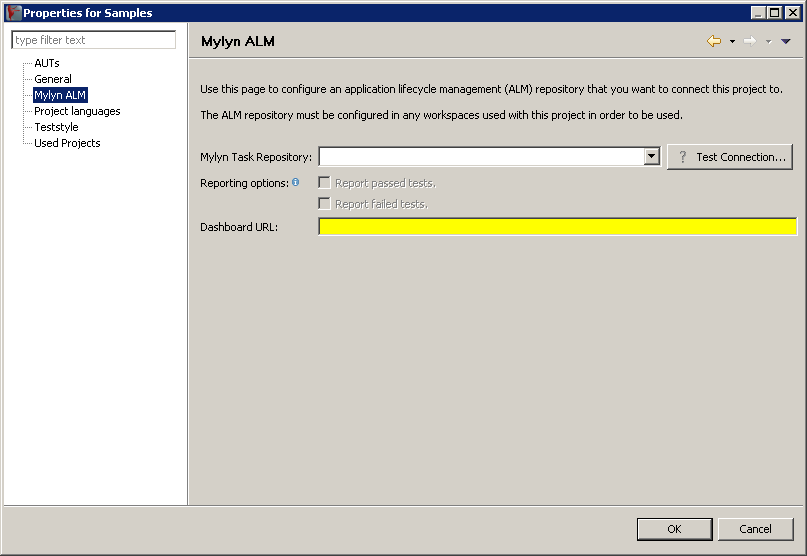
\includegraphics[width=12.5cm]{Tasks/ALM/PS/almproperties}
\caption{ALM Settings}
\label{TasksALMProjectProperties}
\end{center}
\end{figure}


\subsection{Adding task IDs to \gdjobs{}, \gdsuites{} and \gdcases{}}
\label{TasksALMAddTask}
You can add a task ID to \gdcases{}, \gdsuites{} and \gdjobs{} in your \gdproject{}. 

The task ID should be a valid ID in the repository that you have specified as the repository for this \gdproject{} \bxpref{TasksALMConfigureProject}. Adding the task ID to an item in your \gdproject{} means that this item is the relevant test for that task in your repository. When you activate the option, any test results for this item will be added as a comment to the task in the repository. The comment will include a link to the dashboard, in which the test result report can be viewed.

To add a task ID to a \gdcase{}, \gdsuite{} or \gdjob{}:
\begin{enumerate}
\item Open the item in the editor by double-clicking it.
\item In the \gdpropview{}, in the cell for \bxname{Task ID}, enter the task ID from the external repository. You can only enter task IDs at the place of specification -- you cannot overwrite them when you reuse the item.
\item Save the editor. 
\item When you have added a task ID to a node, you can open the task for this node from the browser by selecting:\\
\bxmenu{Open with}{Mylyn Task Editor}{}
\end{enumerate}

\bxtipp{You should ensure that you add task IDs to the right node-level to provide you with the relevant amount of information for the tasks in your repository. This will usually be at the level of Use Cases within a \gdsuite{}. }



\clearpage
\section{Searching in \app{}}
The amount of keywords you have in a \app{} test and the amount of components your test deals with can grow very quickly. For this reason, it is important to think about structuring the \gdtestcasebrowser{} and the \gdomeditor{} to make finding \gdcases{} and component names easier. 


\subsection{Configuring task repositories in your workspace}
\label{TasksALMConfigureWorkspace}
Each repository you want to work with in your \ite{} must be configured in the workspace you are using. 

\begin{enumerate}
\item Select:\\ \bxmenu{Window}{Show View}{Other}\\ from the menu.
\item In the \bxname{Mylyn} section, select \bxname{Task Repositories} and click \bxcaption{OK}. The \bxname{Task Repositories} View will appear. The Bugzilla Repositories for \gd{} and \jb{} are pre-configured.
\item In the \bxname{Task Repositories} View, right click and select \bxname{Add Task Repository} from the context menu.
\item In the dialog that appears, you will see the pre-defined task repositories for the \ite{}. You can select one of these or choose to install a different connector. Depending on the connector you want to use, you may require additional software from Tasktop, or the connector may incur license fees.
\item Once you have selected your connector, click \bxcaption{Next}.
\item On the following page, you will need to configure the task repository. Please refer to the Mylyn documentation for information on repository configuration. 
\item Click \bxcaption{Finish} once the repository is configured.
\item To be able to see tasks in this repository, select: \\ \bxmenu{Window}{Show View}{Other}\\ from the menu. 
\item In the \bxname{Mylyn} section, select \bxname{Task List} and click \bxcaption{OK}. The \bxname{Task List} View will appear.
\end{enumerate}

You will now be able to see items in this repository, open them in the \ite{}, add queries for your workspace and work on tasks from this repository. 
You will also be able to select this repository in the \gdproject{} properties as the repository for your \gdproject{} \bxpref{TasksALMConfigureProject}. 


\subsection{Working on tasks in the \ite{}: contexts}
Once you have configured a task repository for your workspace \bxpref{TasksALMConfigureWorkspace}, you can work on tasks from that repository. 

\subsubsection{Opening and editing tasks in the \ite{}}
\begin{itemize}
\item To be able to see tasks in a repository, select: \\ \bxmenu{Window}{Show View}{Other}\\ from the menu. 
\item In the \bxname{Mylyn} section, select \bxname{Task List} and click \bxcaption{OK}. The \bxname{Task List} View will appear.
\item Double-click on a task to open this task in the editor area.
\item Once a task is open, you can work on it as you would in an external system -- add comments, change status etc.
\end{itemize}

\subsubsection{Working on tasks in the \ite{}}
\label{TasksActivateTask}
Mylyn supports context- or task-based working. When you work on a task, you only see items relevant to that task, so that coming back to the task later involves less context-switching. 
\begin{itemize}
\item Mylyn supports context-based working. You can work on existing tasks in a configured repository, or you can create tasks to work on.
\item To work on a task, you must \bxname{activate} it. To activate a task, select the task in the \bxname{Task List} and select:\\ \bxmenu{Activate}{}{}\\
from the context-sensitive menu. 
\item When you activate a task for the first time, the browsers and editors will seem very empty. This is because nothing is yet a part of the context for this task.
\item You can navigate through the browsers by pressing \bxkey{Alt+Click} to expand each level, or you can press the \bxname{Focus on task} button in the browsers to show the whole tree (not focusing on the task), or just the items in the current context (focusing on the task). 
\item Items are automatically added to your context when you select them in a browser, when you open them in an editor, or when you perform other actions that cause them to be made relevant (e.g. \gdcase{} creation, showing a \gdcase{} specification etc.). Items that are used particularly frequently are marked as \bxname{landmarks} and shown in bold. 
\item You can manually alter which items are in your context using the context-sensitive menu for a specific item. You can manually make items landmarks, or remove them from the context. 
\item The context that is created for you will be re-created when you reactivate the task at a later point. 
\end{itemize}



\subsection{Creating tasks in external repositories from test result reports}
\gdhelpid{testResultViewContextId}{Test Results View}
 You can create a new task with pre-filled information directly from an open test result report in the \gdtestresultview{}. This is useful if a test has failed and you want to create e.g. an issue in your bug-tracking system for the failure. 
\begin{enumerate}
\item In an open test result report, select the node that best describes the test failure (e.g. a \gdcase{} or \gdstep{} that has failed, or the whole \gdsuite{}, then right-click and select:\\
\bxmenu{Create a Mylyn Task}{}{}\\
from the context-sensitive menu.
\item  In the dialog that appears, select a repository in which to create the task. A \bxname{local} repository is available by default, but you can also add connections to Bugzilla and Trac repositories by clicking \bxcaption{Add Task Repository} in the New Task Dialog. Connectors to other repositories can also be added. See the Mylyn documentation for more details on adding repositories.
\item Click \bxcaption{Finish} once you have selected your repository. 
\item The editor for a new task will appear. It is pre-filled with information relevant to the node that you selected. Edit the task to make it descriptive enough for a bug report and save the editor. 
\item Once you have created a task, you can activate it to start saving your context for this task. See the later section \bxpref{TasksActivateTask} for details.
\end{enumerate}


\subsection{Configuring a task repository for your \gdproject{}}
\label{TasksALMConfigureProject}
Once you have configured one or more repositories for your workspace \bxpref{}, you can select one of these to be the test-relevant repository for your \gdproject{}. 

This will let you:
\begin{itemize}
\item Add a task ID from this repository to \gdcases{}, \gdsuites{}, and \gdjobs{} in the \gdproject{} to signify that this item is the test for this task \bxpref{TasksALMAddTask}.
\item Automatically report test results to the task defined when a test runs.
\item View the test results for the relevant item in the dashboard as a link from the task repository.
\end{itemize}

To configure a task repository for your \gdproject{}:

\begin{enumerate}
\item In the \gdproject{} Properties, select \bxname{Mylyn ALM} from the tree on the left \bxfigref{TasksALMProjectProperties}.
\item In the page that appears, you can select a repository from the combo-box.
\item You can then choose whether to only report failed tests, only report successful tests, or both.
\item Enter the URL of the \dash{} that is configured to use the correct \gddb{} for your test results. This is the \dash{} that will be opened when you click on a test result link from the task repository.
\end{enumerate}

\begin{figure}[h]
\begin{center}
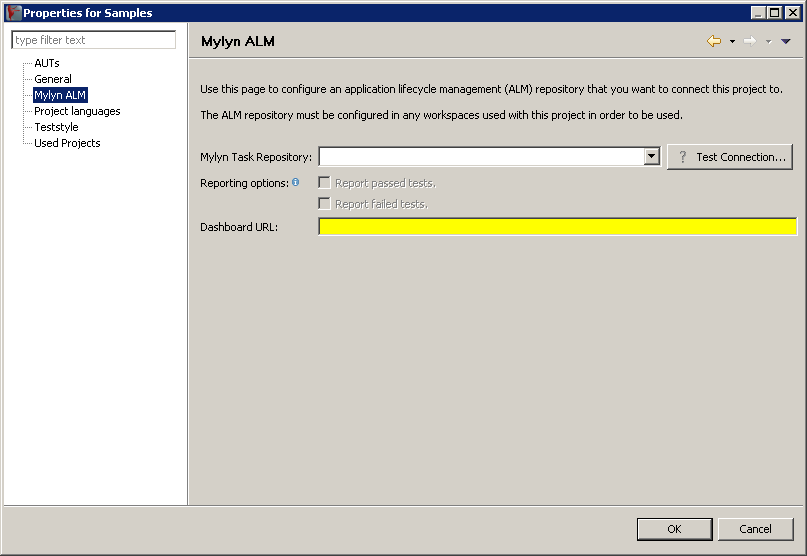
\includegraphics[width=12.5cm]{Tasks/ALM/PS/almproperties}
\caption{ALM Settings}
\label{TasksALMProjectProperties}
\end{center}
\end{figure}


\subsection{Adding task IDs to \gdjobs{}, \gdsuites{} and \gdcases{}}
\label{TasksALMAddTask}
You can add a task ID to \gdcases{}, \gdsuites{} and \gdjobs{} in your \gdproject{}. 

The task ID should be a valid ID in the repository that you have specified as the repository for this \gdproject{} \bxpref{TasksALMConfigureProject}. Adding the task ID to an item in your \gdproject{} means that this item is the relevant test for that task in your repository. When you activate the option, any test results for this item will be added as a comment to the task in the repository. The comment will include a link to the dashboard, in which the test result report can be viewed.

To add a task ID to a \gdcase{}, \gdsuite{} or \gdjob{}:
\begin{enumerate}
\item Open the item in the editor by double-clicking it.
\item In the \gdpropview{}, in the cell for \bxname{Task ID}, enter the task ID from the external repository. You can only enter task IDs at the place of specification -- you cannot overwrite them when you reuse the item.
\item Save the editor. 
\item When you have added a task ID to a node, you can open the task for this node from the browser by selecting:\\
\bxmenu{Open with}{Mylyn Task Editor}{}
\end{enumerate}

\bxtipp{You should ensure that you add task IDs to the right node-level to provide you with the relevant amount of information for the tasks in your repository. This will usually be at the level of Use Cases within a \gdsuite{}. }



\clearpage

\section{Troubleshooting}
The amount of keywords you have in a \app{} test and the amount of components your test deals with can grow very quickly. For this reason, it is important to think about structuring the \gdtestcasebrowser{} and the \gdomeditor{} to make finding \gdcases{} and component names easier. 


\subsection{Configuring task repositories in your workspace}
\label{TasksALMConfigureWorkspace}
Each repository you want to work with in your \ite{} must be configured in the workspace you are using. 

\begin{enumerate}
\item Select:\\ \bxmenu{Window}{Show View}{Other}\\ from the menu.
\item In the \bxname{Mylyn} section, select \bxname{Task Repositories} and click \bxcaption{OK}. The \bxname{Task Repositories} View will appear. The Bugzilla Repositories for \gd{} and \jb{} are pre-configured.
\item In the \bxname{Task Repositories} View, right click and select \bxname{Add Task Repository} from the context menu.
\item In the dialog that appears, you will see the pre-defined task repositories for the \ite{}. You can select one of these or choose to install a different connector. Depending on the connector you want to use, you may require additional software from Tasktop, or the connector may incur license fees.
\item Once you have selected your connector, click \bxcaption{Next}.
\item On the following page, you will need to configure the task repository. Please refer to the Mylyn documentation for information on repository configuration. 
\item Click \bxcaption{Finish} once the repository is configured.
\item To be able to see tasks in this repository, select: \\ \bxmenu{Window}{Show View}{Other}\\ from the menu. 
\item In the \bxname{Mylyn} section, select \bxname{Task List} and click \bxcaption{OK}. The \bxname{Task List} View will appear.
\end{enumerate}

You will now be able to see items in this repository, open them in the \ite{}, add queries for your workspace and work on tasks from this repository. 
You will also be able to select this repository in the \gdproject{} properties as the repository for your \gdproject{} \bxpref{TasksALMConfigureProject}. 


\subsection{Working on tasks in the \ite{}: contexts}
Once you have configured a task repository for your workspace \bxpref{TasksALMConfigureWorkspace}, you can work on tasks from that repository. 

\subsubsection{Opening and editing tasks in the \ite{}}
\begin{itemize}
\item To be able to see tasks in a repository, select: \\ \bxmenu{Window}{Show View}{Other}\\ from the menu. 
\item In the \bxname{Mylyn} section, select \bxname{Task List} and click \bxcaption{OK}. The \bxname{Task List} View will appear.
\item Double-click on a task to open this task in the editor area.
\item Once a task is open, you can work on it as you would in an external system -- add comments, change status etc.
\end{itemize}

\subsubsection{Working on tasks in the \ite{}}
\label{TasksActivateTask}
Mylyn supports context- or task-based working. When you work on a task, you only see items relevant to that task, so that coming back to the task later involves less context-switching. 
\begin{itemize}
\item Mylyn supports context-based working. You can work on existing tasks in a configured repository, or you can create tasks to work on.
\item To work on a task, you must \bxname{activate} it. To activate a task, select the task in the \bxname{Task List} and select:\\ \bxmenu{Activate}{}{}\\
from the context-sensitive menu. 
\item When you activate a task for the first time, the browsers and editors will seem very empty. This is because nothing is yet a part of the context for this task.
\item You can navigate through the browsers by pressing \bxkey{Alt+Click} to expand each level, or you can press the \bxname{Focus on task} button in the browsers to show the whole tree (not focusing on the task), or just the items in the current context (focusing on the task). 
\item Items are automatically added to your context when you select them in a browser, when you open them in an editor, or when you perform other actions that cause them to be made relevant (e.g. \gdcase{} creation, showing a \gdcase{} specification etc.). Items that are used particularly frequently are marked as \bxname{landmarks} and shown in bold. 
\item You can manually alter which items are in your context using the context-sensitive menu for a specific item. You can manually make items landmarks, or remove them from the context. 
\item The context that is created for you will be re-created when you reactivate the task at a later point. 
\end{itemize}



\subsection{Creating tasks in external repositories from test result reports}
\gdhelpid{testResultViewContextId}{Test Results View}
 You can create a new task with pre-filled information directly from an open test result report in the \gdtestresultview{}. This is useful if a test has failed and you want to create e.g. an issue in your bug-tracking system for the failure. 
\begin{enumerate}
\item In an open test result report, select the node that best describes the test failure (e.g. a \gdcase{} or \gdstep{} that has failed, or the whole \gdsuite{}, then right-click and select:\\
\bxmenu{Create a Mylyn Task}{}{}\\
from the context-sensitive menu.
\item  In the dialog that appears, select a repository in which to create the task. A \bxname{local} repository is available by default, but you can also add connections to Bugzilla and Trac repositories by clicking \bxcaption{Add Task Repository} in the New Task Dialog. Connectors to other repositories can also be added. See the Mylyn documentation for more details on adding repositories.
\item Click \bxcaption{Finish} once you have selected your repository. 
\item The editor for a new task will appear. It is pre-filled with information relevant to the node that you selected. Edit the task to make it descriptive enough for a bug report and save the editor. 
\item Once you have created a task, you can activate it to start saving your context for this task. See the later section \bxpref{TasksActivateTask} for details.
\end{enumerate}


\subsection{Configuring a task repository for your \gdproject{}}
\label{TasksALMConfigureProject}
Once you have configured one or more repositories for your workspace \bxpref{}, you can select one of these to be the test-relevant repository for your \gdproject{}. 

This will let you:
\begin{itemize}
\item Add a task ID from this repository to \gdcases{}, \gdsuites{}, and \gdjobs{} in the \gdproject{} to signify that this item is the test for this task \bxpref{TasksALMAddTask}.
\item Automatically report test results to the task defined when a test runs.
\item View the test results for the relevant item in the dashboard as a link from the task repository.
\end{itemize}

To configure a task repository for your \gdproject{}:

\begin{enumerate}
\item In the \gdproject{} Properties, select \bxname{Mylyn ALM} from the tree on the left \bxfigref{TasksALMProjectProperties}.
\item In the page that appears, you can select a repository from the combo-box.
\item You can then choose whether to only report failed tests, only report successful tests, or both.
\item Enter the URL of the \dash{} that is configured to use the correct \gddb{} for your test results. This is the \dash{} that will be opened when you click on a test result link from the task repository.
\end{enumerate}

\begin{figure}[h]
\begin{center}
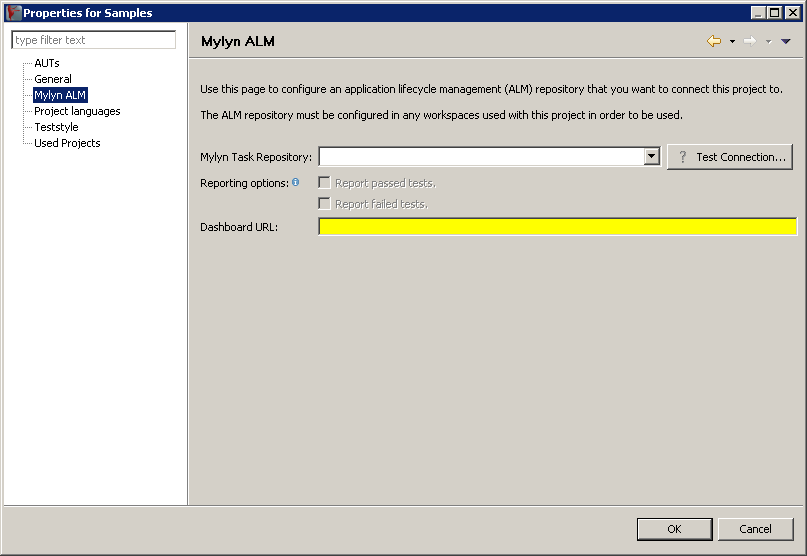
\includegraphics[width=12.5cm]{Tasks/ALM/PS/almproperties}
\caption{ALM Settings}
\label{TasksALMProjectProperties}
\end{center}
\end{figure}


\subsection{Adding task IDs to \gdjobs{}, \gdsuites{} and \gdcases{}}
\label{TasksALMAddTask}
You can add a task ID to \gdcases{}, \gdsuites{} and \gdjobs{} in your \gdproject{}. 

The task ID should be a valid ID in the repository that you have specified as the repository for this \gdproject{} \bxpref{TasksALMConfigureProject}. Adding the task ID to an item in your \gdproject{} means that this item is the relevant test for that task in your repository. When you activate the option, any test results for this item will be added as a comment to the task in the repository. The comment will include a link to the dashboard, in which the test result report can be viewed.

To add a task ID to a \gdcase{}, \gdsuite{} or \gdjob{}:
\begin{enumerate}
\item Open the item in the editor by double-clicking it.
\item In the \gdpropview{}, in the cell for \bxname{Task ID}, enter the task ID from the external repository. You can only enter task IDs at the place of specification -- you cannot overwrite them when you reuse the item.
\item Save the editor. 
\item When you have added a task ID to a node, you can open the task for this node from the browser by selecting:\\
\bxmenu{Open with}{Mylyn Task Editor}{}
\end{enumerate}

\bxtipp{You should ensure that you add task IDs to the right node-level to provide you with the relevant amount of information for the tasks in your repository. This will usually be at the level of Use Cases within a \gdsuite{}. }




\clearpage

\section{Finishing up}
The amount of keywords you have in a \app{} test and the amount of components your test deals with can grow very quickly. For this reason, it is important to think about structuring the \gdtestcasebrowser{} and the \gdomeditor{} to make finding \gdcases{} and component names easier. 


\subsection{Configuring task repositories in your workspace}
\label{TasksALMConfigureWorkspace}
Each repository you want to work with in your \ite{} must be configured in the workspace you are using. 

\begin{enumerate}
\item Select:\\ \bxmenu{Window}{Show View}{Other}\\ from the menu.
\item In the \bxname{Mylyn} section, select \bxname{Task Repositories} and click \bxcaption{OK}. The \bxname{Task Repositories} View will appear. The Bugzilla Repositories for \gd{} and \jb{} are pre-configured.
\item In the \bxname{Task Repositories} View, right click and select \bxname{Add Task Repository} from the context menu.
\item In the dialog that appears, you will see the pre-defined task repositories for the \ite{}. You can select one of these or choose to install a different connector. Depending on the connector you want to use, you may require additional software from Tasktop, or the connector may incur license fees.
\item Once you have selected your connector, click \bxcaption{Next}.
\item On the following page, you will need to configure the task repository. Please refer to the Mylyn documentation for information on repository configuration. 
\item Click \bxcaption{Finish} once the repository is configured.
\item To be able to see tasks in this repository, select: \\ \bxmenu{Window}{Show View}{Other}\\ from the menu. 
\item In the \bxname{Mylyn} section, select \bxname{Task List} and click \bxcaption{OK}. The \bxname{Task List} View will appear.
\end{enumerate}

You will now be able to see items in this repository, open them in the \ite{}, add queries for your workspace and work on tasks from this repository. 
You will also be able to select this repository in the \gdproject{} properties as the repository for your \gdproject{} \bxpref{TasksALMConfigureProject}. 


\subsection{Working on tasks in the \ite{}: contexts}
Once you have configured a task repository for your workspace \bxpref{TasksALMConfigureWorkspace}, you can work on tasks from that repository. 

\subsubsection{Opening and editing tasks in the \ite{}}
\begin{itemize}
\item To be able to see tasks in a repository, select: \\ \bxmenu{Window}{Show View}{Other}\\ from the menu. 
\item In the \bxname{Mylyn} section, select \bxname{Task List} and click \bxcaption{OK}. The \bxname{Task List} View will appear.
\item Double-click on a task to open this task in the editor area.
\item Once a task is open, you can work on it as you would in an external system -- add comments, change status etc.
\end{itemize}

\subsubsection{Working on tasks in the \ite{}}
\label{TasksActivateTask}
Mylyn supports context- or task-based working. When you work on a task, you only see items relevant to that task, so that coming back to the task later involves less context-switching. 
\begin{itemize}
\item Mylyn supports context-based working. You can work on existing tasks in a configured repository, or you can create tasks to work on.
\item To work on a task, you must \bxname{activate} it. To activate a task, select the task in the \bxname{Task List} and select:\\ \bxmenu{Activate}{}{}\\
from the context-sensitive menu. 
\item When you activate a task for the first time, the browsers and editors will seem very empty. This is because nothing is yet a part of the context for this task.
\item You can navigate through the browsers by pressing \bxkey{Alt+Click} to expand each level, or you can press the \bxname{Focus on task} button in the browsers to show the whole tree (not focusing on the task), or just the items in the current context (focusing on the task). 
\item Items are automatically added to your context when you select them in a browser, when you open them in an editor, or when you perform other actions that cause them to be made relevant (e.g. \gdcase{} creation, showing a \gdcase{} specification etc.). Items that are used particularly frequently are marked as \bxname{landmarks} and shown in bold. 
\item You can manually alter which items are in your context using the context-sensitive menu for a specific item. You can manually make items landmarks, or remove them from the context. 
\item The context that is created for you will be re-created when you reactivate the task at a later point. 
\end{itemize}



\subsection{Creating tasks in external repositories from test result reports}
\gdhelpid{testResultViewContextId}{Test Results View}
 You can create a new task with pre-filled information directly from an open test result report in the \gdtestresultview{}. This is useful if a test has failed and you want to create e.g. an issue in your bug-tracking system for the failure. 
\begin{enumerate}
\item In an open test result report, select the node that best describes the test failure (e.g. a \gdcase{} or \gdstep{} that has failed, or the whole \gdsuite{}, then right-click and select:\\
\bxmenu{Create a Mylyn Task}{}{}\\
from the context-sensitive menu.
\item  In the dialog that appears, select a repository in which to create the task. A \bxname{local} repository is available by default, but you can also add connections to Bugzilla and Trac repositories by clicking \bxcaption{Add Task Repository} in the New Task Dialog. Connectors to other repositories can also be added. See the Mylyn documentation for more details on adding repositories.
\item Click \bxcaption{Finish} once you have selected your repository. 
\item The editor for a new task will appear. It is pre-filled with information relevant to the node that you selected. Edit the task to make it descriptive enough for a bug report and save the editor. 
\item Once you have created a task, you can activate it to start saving your context for this task. See the later section \bxpref{TasksActivateTask} for details.
\end{enumerate}


\subsection{Configuring a task repository for your \gdproject{}}
\label{TasksALMConfigureProject}
Once you have configured one or more repositories for your workspace \bxpref{}, you can select one of these to be the test-relevant repository for your \gdproject{}. 

This will let you:
\begin{itemize}
\item Add a task ID from this repository to \gdcases{}, \gdsuites{}, and \gdjobs{} in the \gdproject{} to signify that this item is the test for this task \bxpref{TasksALMAddTask}.
\item Automatically report test results to the task defined when a test runs.
\item View the test results for the relevant item in the dashboard as a link from the task repository.
\end{itemize}

To configure a task repository for your \gdproject{}:

\begin{enumerate}
\item In the \gdproject{} Properties, select \bxname{Mylyn ALM} from the tree on the left \bxfigref{TasksALMProjectProperties}.
\item In the page that appears, you can select a repository from the combo-box.
\item You can then choose whether to only report failed tests, only report successful tests, or both.
\item Enter the URL of the \dash{} that is configured to use the correct \gddb{} for your test results. This is the \dash{} that will be opened when you click on a test result link from the task repository.
\end{enumerate}

\begin{figure}[h]
\begin{center}
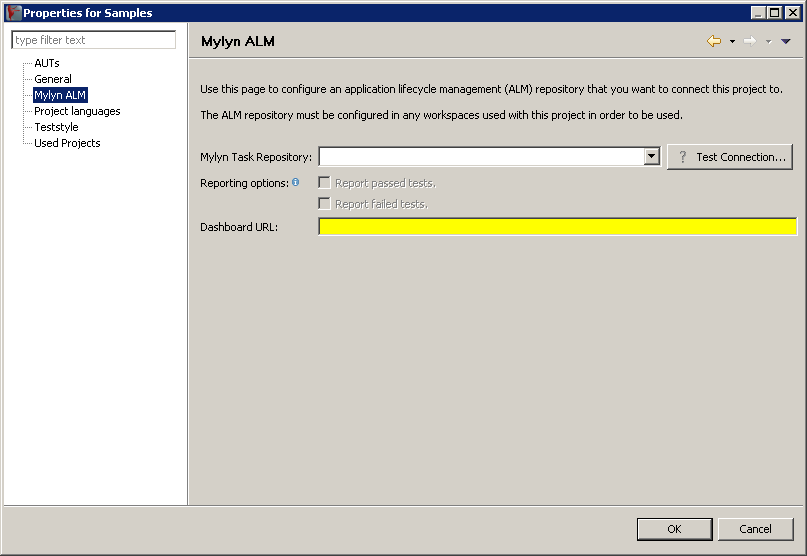
\includegraphics[width=12.5cm]{Tasks/ALM/PS/almproperties}
\caption{ALM Settings}
\label{TasksALMProjectProperties}
\end{center}
\end{figure}


\subsection{Adding task IDs to \gdjobs{}, \gdsuites{} and \gdcases{}}
\label{TasksALMAddTask}
You can add a task ID to \gdcases{}, \gdsuites{} and \gdjobs{} in your \gdproject{}. 

The task ID should be a valid ID in the repository that you have specified as the repository for this \gdproject{} \bxpref{TasksALMConfigureProject}. Adding the task ID to an item in your \gdproject{} means that this item is the relevant test for that task in your repository. When you activate the option, any test results for this item will be added as a comment to the task in the repository. The comment will include a link to the dashboard, in which the test result report can be viewed.

To add a task ID to a \gdcase{}, \gdsuite{} or \gdjob{}:
\begin{enumerate}
\item Open the item in the editor by double-clicking it.
\item In the \gdpropview{}, in the cell for \bxname{Task ID}, enter the task ID from the external repository. You can only enter task IDs at the place of specification -- you cannot overwrite them when you reuse the item.
\item Save the editor. 
\item When you have added a task ID to a node, you can open the task for this node from the browser by selecting:\\
\bxmenu{Open with}{Mylyn Task Editor}{}
\end{enumerate}

\bxtipp{You should ensure that you add task IDs to the right node-level to provide you with the relevant amount of information for the tasks in your repository. This will usually be at the level of Use Cases within a \gdsuite{}. }




\clearpage

\section{Using the test executor}
\gdhelpid{problemViewContextId}{Problem View}
The amount of keywords you have in a \app{} test and the amount of components your test deals with can grow very quickly. For this reason, it is important to think about structuring the \gdtestcasebrowser{} and the \gdomeditor{} to make finding \gdcases{} and component names easier. 


\subsection{Configuring task repositories in your workspace}
\label{TasksALMConfigureWorkspace}
Each repository you want to work with in your \ite{} must be configured in the workspace you are using. 

\begin{enumerate}
\item Select:\\ \bxmenu{Window}{Show View}{Other}\\ from the menu.
\item In the \bxname{Mylyn} section, select \bxname{Task Repositories} and click \bxcaption{OK}. The \bxname{Task Repositories} View will appear. The Bugzilla Repositories for \gd{} and \jb{} are pre-configured.
\item In the \bxname{Task Repositories} View, right click and select \bxname{Add Task Repository} from the context menu.
\item In the dialog that appears, you will see the pre-defined task repositories for the \ite{}. You can select one of these or choose to install a different connector. Depending on the connector you want to use, you may require additional software from Tasktop, or the connector may incur license fees.
\item Once you have selected your connector, click \bxcaption{Next}.
\item On the following page, you will need to configure the task repository. Please refer to the Mylyn documentation for information on repository configuration. 
\item Click \bxcaption{Finish} once the repository is configured.
\item To be able to see tasks in this repository, select: \\ \bxmenu{Window}{Show View}{Other}\\ from the menu. 
\item In the \bxname{Mylyn} section, select \bxname{Task List} and click \bxcaption{OK}. The \bxname{Task List} View will appear.
\end{enumerate}

You will now be able to see items in this repository, open them in the \ite{}, add queries for your workspace and work on tasks from this repository. 
You will also be able to select this repository in the \gdproject{} properties as the repository for your \gdproject{} \bxpref{TasksALMConfigureProject}. 


\subsection{Working on tasks in the \ite{}: contexts}
Once you have configured a task repository for your workspace \bxpref{TasksALMConfigureWorkspace}, you can work on tasks from that repository. 

\subsubsection{Opening and editing tasks in the \ite{}}
\begin{itemize}
\item To be able to see tasks in a repository, select: \\ \bxmenu{Window}{Show View}{Other}\\ from the menu. 
\item In the \bxname{Mylyn} section, select \bxname{Task List} and click \bxcaption{OK}. The \bxname{Task List} View will appear.
\item Double-click on a task to open this task in the editor area.
\item Once a task is open, you can work on it as you would in an external system -- add comments, change status etc.
\end{itemize}

\subsubsection{Working on tasks in the \ite{}}
\label{TasksActivateTask}
Mylyn supports context- or task-based working. When you work on a task, you only see items relevant to that task, so that coming back to the task later involves less context-switching. 
\begin{itemize}
\item Mylyn supports context-based working. You can work on existing tasks in a configured repository, or you can create tasks to work on.
\item To work on a task, you must \bxname{activate} it. To activate a task, select the task in the \bxname{Task List} and select:\\ \bxmenu{Activate}{}{}\\
from the context-sensitive menu. 
\item When you activate a task for the first time, the browsers and editors will seem very empty. This is because nothing is yet a part of the context for this task.
\item You can navigate through the browsers by pressing \bxkey{Alt+Click} to expand each level, or you can press the \bxname{Focus on task} button in the browsers to show the whole tree (not focusing on the task), or just the items in the current context (focusing on the task). 
\item Items are automatically added to your context when you select them in a browser, when you open them in an editor, or when you perform other actions that cause them to be made relevant (e.g. \gdcase{} creation, showing a \gdcase{} specification etc.). Items that are used particularly frequently are marked as \bxname{landmarks} and shown in bold. 
\item You can manually alter which items are in your context using the context-sensitive menu for a specific item. You can manually make items landmarks, or remove them from the context. 
\item The context that is created for you will be re-created when you reactivate the task at a later point. 
\end{itemize}



\subsection{Creating tasks in external repositories from test result reports}
\gdhelpid{testResultViewContextId}{Test Results View}
 You can create a new task with pre-filled information directly from an open test result report in the \gdtestresultview{}. This is useful if a test has failed and you want to create e.g. an issue in your bug-tracking system for the failure. 
\begin{enumerate}
\item In an open test result report, select the node that best describes the test failure (e.g. a \gdcase{} or \gdstep{} that has failed, or the whole \gdsuite{}, then right-click and select:\\
\bxmenu{Create a Mylyn Task}{}{}\\
from the context-sensitive menu.
\item  In the dialog that appears, select a repository in which to create the task. A \bxname{local} repository is available by default, but you can also add connections to Bugzilla and Trac repositories by clicking \bxcaption{Add Task Repository} in the New Task Dialog. Connectors to other repositories can also be added. See the Mylyn documentation for more details on adding repositories.
\item Click \bxcaption{Finish} once you have selected your repository. 
\item The editor for a new task will appear. It is pre-filled with information relevant to the node that you selected. Edit the task to make it descriptive enough for a bug report and save the editor. 
\item Once you have created a task, you can activate it to start saving your context for this task. See the later section \bxpref{TasksActivateTask} for details.
\end{enumerate}


\subsection{Configuring a task repository for your \gdproject{}}
\label{TasksALMConfigureProject}
Once you have configured one or more repositories for your workspace \bxpref{}, you can select one of these to be the test-relevant repository for your \gdproject{}. 

This will let you:
\begin{itemize}
\item Add a task ID from this repository to \gdcases{}, \gdsuites{}, and \gdjobs{} in the \gdproject{} to signify that this item is the test for this task \bxpref{TasksALMAddTask}.
\item Automatically report test results to the task defined when a test runs.
\item View the test results for the relevant item in the dashboard as a link from the task repository.
\end{itemize}

To configure a task repository for your \gdproject{}:

\begin{enumerate}
\item In the \gdproject{} Properties, select \bxname{Mylyn ALM} from the tree on the left \bxfigref{TasksALMProjectProperties}.
\item In the page that appears, you can select a repository from the combo-box.
\item You can then choose whether to only report failed tests, only report successful tests, or both.
\item Enter the URL of the \dash{} that is configured to use the correct \gddb{} for your test results. This is the \dash{} that will be opened when you click on a test result link from the task repository.
\end{enumerate}

\begin{figure}[h]
\begin{center}
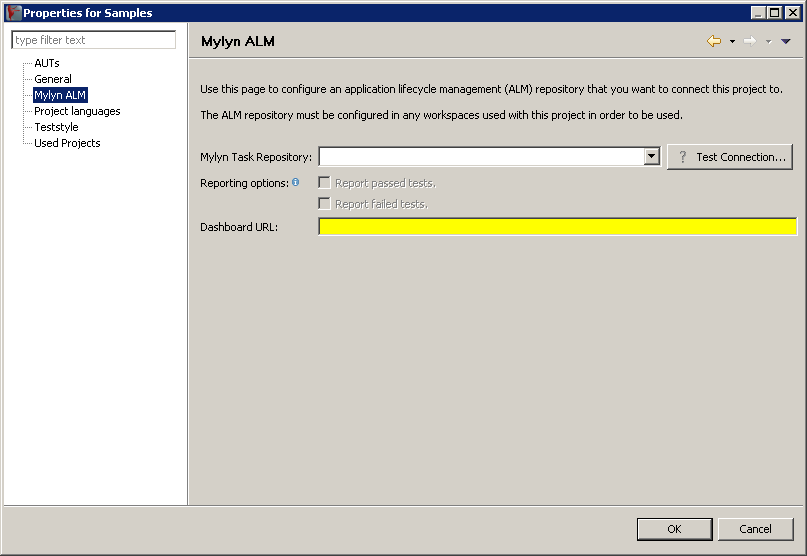
\includegraphics[width=12.5cm]{Tasks/ALM/PS/almproperties}
\caption{ALM Settings}
\label{TasksALMProjectProperties}
\end{center}
\end{figure}


\subsection{Adding task IDs to \gdjobs{}, \gdsuites{} and \gdcases{}}
\label{TasksALMAddTask}
You can add a task ID to \gdcases{}, \gdsuites{} and \gdjobs{} in your \gdproject{}. 

The task ID should be a valid ID in the repository that you have specified as the repository for this \gdproject{} \bxpref{TasksALMConfigureProject}. Adding the task ID to an item in your \gdproject{} means that this item is the relevant test for that task in your repository. When you activate the option, any test results for this item will be added as a comment to the task in the repository. The comment will include a link to the dashboard, in which the test result report can be viewed.

To add a task ID to a \gdcase{}, \gdsuite{} or \gdjob{}:
\begin{enumerate}
\item Open the item in the editor by double-clicking it.
\item In the \gdpropview{}, in the cell for \bxname{Task ID}, enter the task ID from the external repository. You can only enter task IDs at the place of specification -- you cannot overwrite them when you reuse the item.
\item Save the editor. 
\item When you have added a task ID to a node, you can open the task for this node from the browser by selecting:\\
\bxmenu{Open with}{Mylyn Task Editor}{}
\end{enumerate}

\bxtipp{You should ensure that you add task IDs to the right node-level to provide you with the relevant amount of information for the tasks in your repository. This will usually be at the level of Use Cases within a \gdsuite{}. }




\section{Using the dbtool client}
\gdhelpid{problemViewContextId}{Problem View}
\label{DBTool}
The amount of keywords you have in a \app{} test and the amount of components your test deals with can grow very quickly. For this reason, it is important to think about structuring the \gdtestcasebrowser{} and the \gdomeditor{} to make finding \gdcases{} and component names easier. 


\subsection{Configuring task repositories in your workspace}
\label{TasksALMConfigureWorkspace}
Each repository you want to work with in your \ite{} must be configured in the workspace you are using. 

\begin{enumerate}
\item Select:\\ \bxmenu{Window}{Show View}{Other}\\ from the menu.
\item In the \bxname{Mylyn} section, select \bxname{Task Repositories} and click \bxcaption{OK}. The \bxname{Task Repositories} View will appear. The Bugzilla Repositories for \gd{} and \jb{} are pre-configured.
\item In the \bxname{Task Repositories} View, right click and select \bxname{Add Task Repository} from the context menu.
\item In the dialog that appears, you will see the pre-defined task repositories for the \ite{}. You can select one of these or choose to install a different connector. Depending on the connector you want to use, you may require additional software from Tasktop, or the connector may incur license fees.
\item Once you have selected your connector, click \bxcaption{Next}.
\item On the following page, you will need to configure the task repository. Please refer to the Mylyn documentation for information on repository configuration. 
\item Click \bxcaption{Finish} once the repository is configured.
\item To be able to see tasks in this repository, select: \\ \bxmenu{Window}{Show View}{Other}\\ from the menu. 
\item In the \bxname{Mylyn} section, select \bxname{Task List} and click \bxcaption{OK}. The \bxname{Task List} View will appear.
\end{enumerate}

You will now be able to see items in this repository, open them in the \ite{}, add queries for your workspace and work on tasks from this repository. 
You will also be able to select this repository in the \gdproject{} properties as the repository for your \gdproject{} \bxpref{TasksALMConfigureProject}. 


\subsection{Working on tasks in the \ite{}: contexts}
Once you have configured a task repository for your workspace \bxpref{TasksALMConfigureWorkspace}, you can work on tasks from that repository. 

\subsubsection{Opening and editing tasks in the \ite{}}
\begin{itemize}
\item To be able to see tasks in a repository, select: \\ \bxmenu{Window}{Show View}{Other}\\ from the menu. 
\item In the \bxname{Mylyn} section, select \bxname{Task List} and click \bxcaption{OK}. The \bxname{Task List} View will appear.
\item Double-click on a task to open this task in the editor area.
\item Once a task is open, you can work on it as you would in an external system -- add comments, change status etc.
\end{itemize}

\subsubsection{Working on tasks in the \ite{}}
\label{TasksActivateTask}
Mylyn supports context- or task-based working. When you work on a task, you only see items relevant to that task, so that coming back to the task later involves less context-switching. 
\begin{itemize}
\item Mylyn supports context-based working. You can work on existing tasks in a configured repository, or you can create tasks to work on.
\item To work on a task, you must \bxname{activate} it. To activate a task, select the task in the \bxname{Task List} and select:\\ \bxmenu{Activate}{}{}\\
from the context-sensitive menu. 
\item When you activate a task for the first time, the browsers and editors will seem very empty. This is because nothing is yet a part of the context for this task.
\item You can navigate through the browsers by pressing \bxkey{Alt+Click} to expand each level, or you can press the \bxname{Focus on task} button in the browsers to show the whole tree (not focusing on the task), or just the items in the current context (focusing on the task). 
\item Items are automatically added to your context when you select them in a browser, when you open them in an editor, or when you perform other actions that cause them to be made relevant (e.g. \gdcase{} creation, showing a \gdcase{} specification etc.). Items that are used particularly frequently are marked as \bxname{landmarks} and shown in bold. 
\item You can manually alter which items are in your context using the context-sensitive menu for a specific item. You can manually make items landmarks, or remove them from the context. 
\item The context that is created for you will be re-created when you reactivate the task at a later point. 
\end{itemize}



\subsection{Creating tasks in external repositories from test result reports}
\gdhelpid{testResultViewContextId}{Test Results View}
 You can create a new task with pre-filled information directly from an open test result report in the \gdtestresultview{}. This is useful if a test has failed and you want to create e.g. an issue in your bug-tracking system for the failure. 
\begin{enumerate}
\item In an open test result report, select the node that best describes the test failure (e.g. a \gdcase{} or \gdstep{} that has failed, or the whole \gdsuite{}, then right-click and select:\\
\bxmenu{Create a Mylyn Task}{}{}\\
from the context-sensitive menu.
\item  In the dialog that appears, select a repository in which to create the task. A \bxname{local} repository is available by default, but you can also add connections to Bugzilla and Trac repositories by clicking \bxcaption{Add Task Repository} in the New Task Dialog. Connectors to other repositories can also be added. See the Mylyn documentation for more details on adding repositories.
\item Click \bxcaption{Finish} once you have selected your repository. 
\item The editor for a new task will appear. It is pre-filled with information relevant to the node that you selected. Edit the task to make it descriptive enough for a bug report and save the editor. 
\item Once you have created a task, you can activate it to start saving your context for this task. See the later section \bxpref{TasksActivateTask} for details.
\end{enumerate}


\subsection{Configuring a task repository for your \gdproject{}}
\label{TasksALMConfigureProject}
Once you have configured one or more repositories for your workspace \bxpref{}, you can select one of these to be the test-relevant repository for your \gdproject{}. 

This will let you:
\begin{itemize}
\item Add a task ID from this repository to \gdcases{}, \gdsuites{}, and \gdjobs{} in the \gdproject{} to signify that this item is the test for this task \bxpref{TasksALMAddTask}.
\item Automatically report test results to the task defined when a test runs.
\item View the test results for the relevant item in the dashboard as a link from the task repository.
\end{itemize}

To configure a task repository for your \gdproject{}:

\begin{enumerate}
\item In the \gdproject{} Properties, select \bxname{Mylyn ALM} from the tree on the left \bxfigref{TasksALMProjectProperties}.
\item In the page that appears, you can select a repository from the combo-box.
\item You can then choose whether to only report failed tests, only report successful tests, or both.
\item Enter the URL of the \dash{} that is configured to use the correct \gddb{} for your test results. This is the \dash{} that will be opened when you click on a test result link from the task repository.
\end{enumerate}

\begin{figure}[h]
\begin{center}
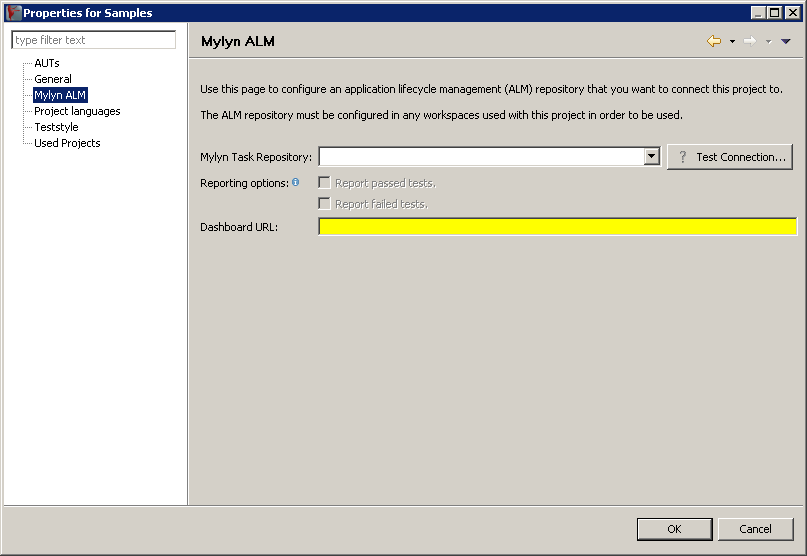
\includegraphics[width=12.5cm]{Tasks/ALM/PS/almproperties}
\caption{ALM Settings}
\label{TasksALMProjectProperties}
\end{center}
\end{figure}


\subsection{Adding task IDs to \gdjobs{}, \gdsuites{} and \gdcases{}}
\label{TasksALMAddTask}
You can add a task ID to \gdcases{}, \gdsuites{} and \gdjobs{} in your \gdproject{}. 

The task ID should be a valid ID in the repository that you have specified as the repository for this \gdproject{} \bxpref{TasksALMConfigureProject}. Adding the task ID to an item in your \gdproject{} means that this item is the relevant test for that task in your repository. When you activate the option, any test results for this item will be added as a comment to the task in the repository. The comment will include a link to the dashboard, in which the test result report can be viewed.

To add a task ID to a \gdcase{}, \gdsuite{} or \gdjob{}:
\begin{enumerate}
\item Open the item in the editor by double-clicking it.
\item In the \gdpropview{}, in the cell for \bxname{Task ID}, enter the task ID from the external repository. You can only enter task IDs at the place of specification -- you cannot overwrite them when you reuse the item.
\item Save the editor. 
\item When you have added a task ID to a node, you can open the task for this node from the browser by selecting:\\
\bxmenu{Open with}{Mylyn Task Editor}{}
\end{enumerate}

\bxtipp{You should ensure that you add task IDs to the right node-level to provide you with the relevant amount of information for the tasks in your repository. This will usually be at the level of Use Cases within a \gdsuite{}. }




